% !TEX root = trackjet_intnote.tex

A description of the analysis procedure to reconstruct the $\Dptr$ distribution, along with the derivation and application of the various corrections is presented in the following sections. The analysis structure is illustrated by the diagram in Fig.~\ref{Fig:analysis_flow} where each part of the analyses is described in a separate subsection and it can be summarized as follows: 


\begin{itemize}
\item Jet selection and calibration
\item Track selection
\item Track momentum correction
\item Fake rates
\item Tracking efficiency
\item Underlying event subtraction of tracks
\item Unfolding
\end{itemize}


\subsection{Jet Selection and final energy calibration}
\label{Sec:JetSelection}
Since the Inner Detector (ID) covers the $|\eta| < 2.5$, the analysis can 
only be performed for jets within the pseudorapidity interval of $|\eta| < 1.3$ to have the entire $r=$1.2 cone under investigation fully covered by the tracking detector. In both collision systems, jets are 
measured with \ptjet\ between 126~GeV and 316~GeV in following four successive intervals: 126--158, 158--200, 200--251, and 251--316~GeV. This binning was motivated by the large fake rate below 100 \GeV. An underflow bin was also needed for the unfolding procedure, and hence, the measurement starts at 126 \GeV. This binning is also used in previous heavy ion jet measurements (\cite{ATLAS502FFConf}). Truth jets were associated with the nearest reconstructed jet using the matching of the $\dR<0.2$ for the performance study and to build response matrices for the unfolding procedure. The same \dR\ matching criteria were employed in previous ATLAS HI jet analyses and are justified by a detailed performance study~\cite{Aad:12081967v1}. To prevent nearby jets from distorting the measurement of \Dptr\ distributions, 
jets are rejected if there is another jet with a higher \ptjet\ than the considered jet anywhere
within a distance of $\Delta R < 1.0$. The isolation cut removes approximately 0.01\% of jets (see Figure \ref{fig:ISO}), and has almost no impact on the final measurement.

\begin{figure}
\centering{
\begin{tabular}{cc}
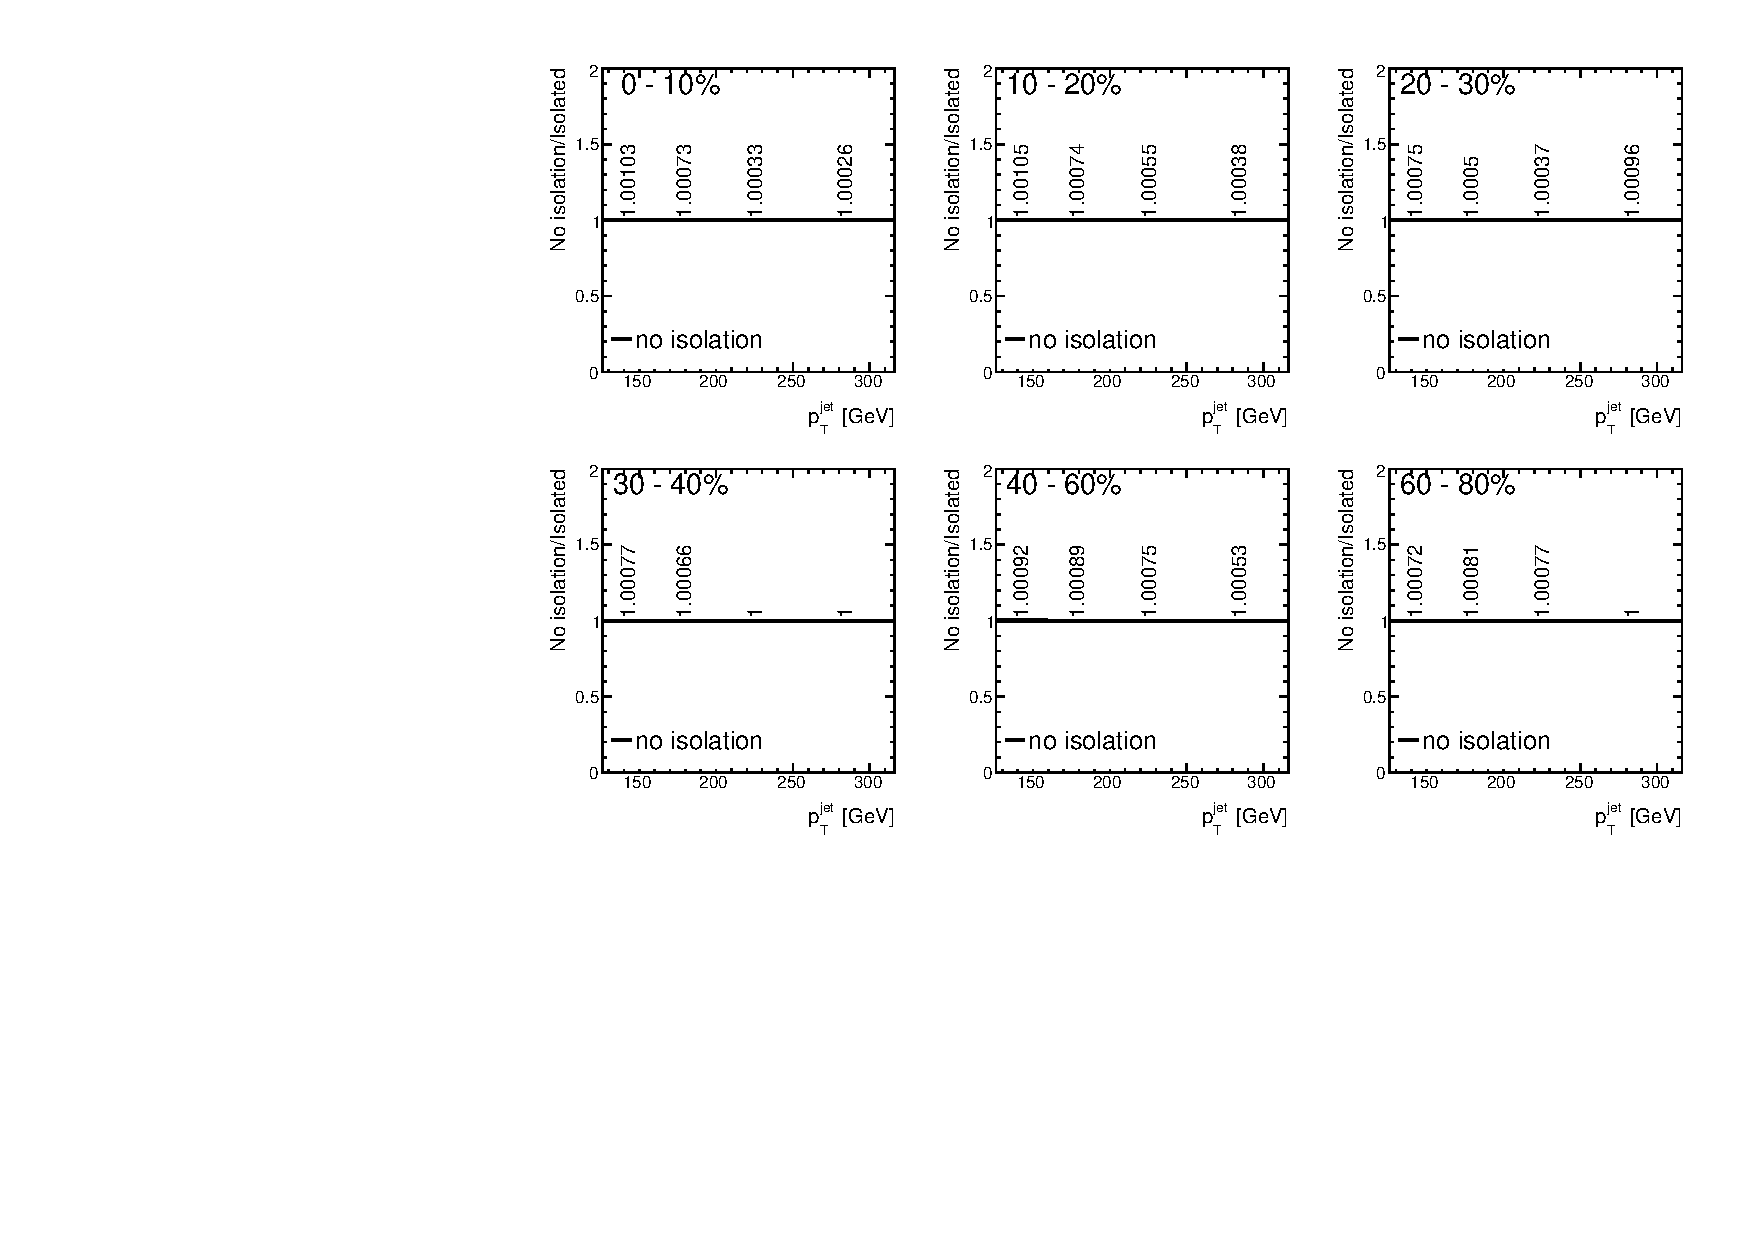
\includegraphics[width=0.9\textwidth]{figures_performance/jet_iso.pdf} \\
\end{tabular}}
\caption{The ratios of the jet spectra with no isolation to that with isolation in the kinematic range of interest for \pbpb\ collisions, in all centralities. The isolation requirement rejects less that 0.1\% of jets, and has almost no impact on the final measurement}
\label{fig:ISO}
\end{figure}  




A final calibration, referred to as a cross-calibration��~\cite{cc2015}, 
was applied to the data to account for observed differences in the calorimetric response between data and MC. The cross-calibration factors were estimated using in-situ calibration studies~\cite{HIjesnote} where jets are measured in events while recoiling against objects for which the energy scale is well known. 
No correction for the jet reconstruction efficiency is necessary, as the analysis is performed in the jet \pT\ region where the jet reconstruction is fully efficient~\cite{ATLAS-COM-PHYS-2013-1369}. 

The jet energy measured in the calorimeter can be affected by the presence 
of dead cells or cells with a bad response, by noise spikes in the hadronic end-cap, by a noise in EM calorimeter and by out-of-time energy deposits from cosmic rays and beam backgrounds. In the \pp\ analysis, the set of recommended cuts of ``LooseBad'' is used to remove bad jets. The rate of these jets in the kinematic region of interest (100--316 \GeV) is less than 0.5\%. This cleaning procedure is not applied in \PbPb\ collisions because it is incompatible with the heavy ion jet reconstruction procedue, and also because the low luminosity ensures noise bursts are negligible. This is standard procedure for all heavy ion jet analyses.
 

%\subsection{Jet isolation}
%
%Jets were required to be isolated. Any jet having another jet with higher 
%\pt\ than the original jet within $\Delta R < 1.0$ has been discarded. Jet isolation has been required in 
%order to not bias the fragmentation measurement by a potential presence of 
%split jets. The procedure is adopted from the fragmentation analyses in \pp~\cite{Aad:2011sc,FF7TeVInt}. 
%
%To test the sensitivity of this requirement, the \pT\ threshold on the second jet within $\Delta R < 1.0$ was decreased to 80\% of the original jet. The ratios of the raw fragmentation functions with the default cut to version with the more strict isolation requirement applied is shown in Fig~\ref{fig:ISO80}. The impact of this correction is small and the difference in the measured distributions is less than 1\%.

%\begin{figure}
%\centering{
%\begin{tabular}{cc}
%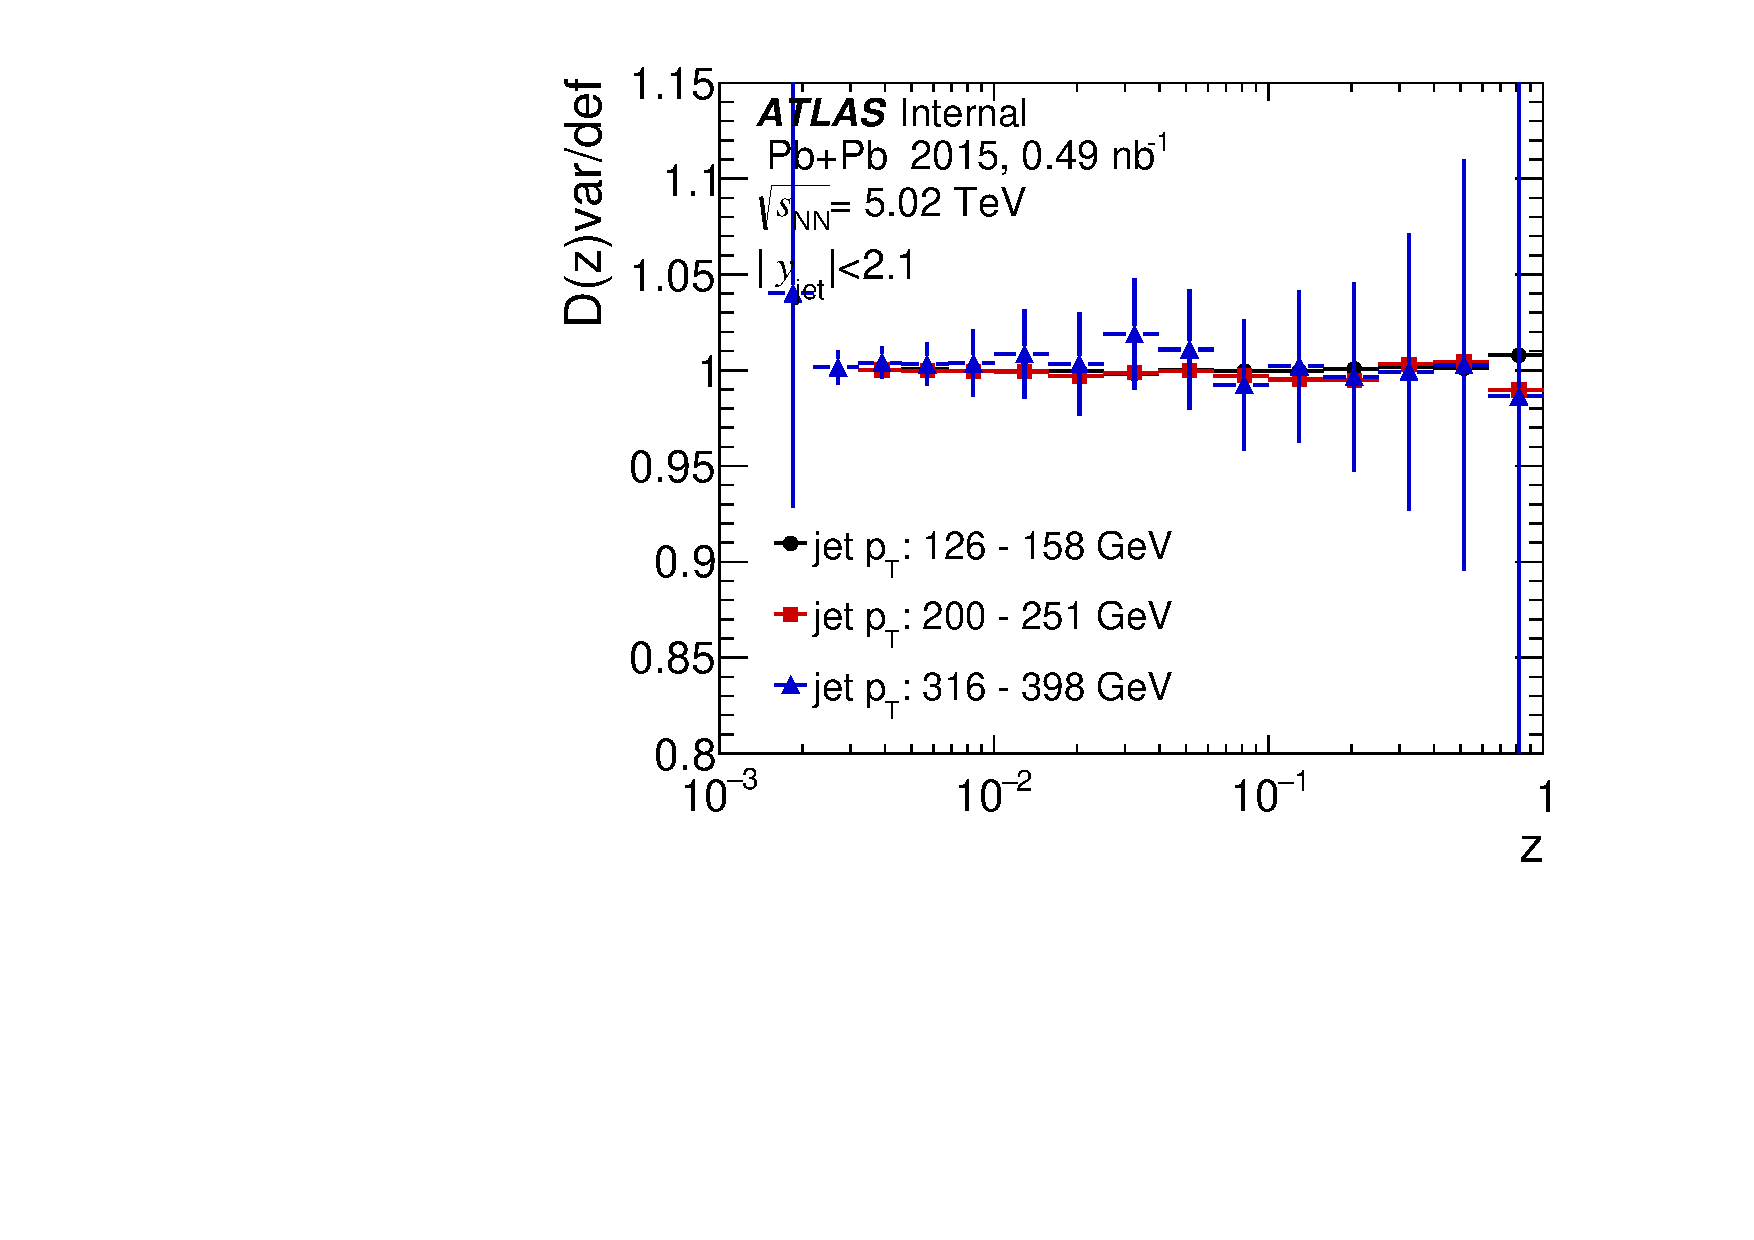
\includegraphics[width=0.45\textwidth]{figures_corrections/ff_data_comaparison_eta4_cent0_iso08.pdf} &
%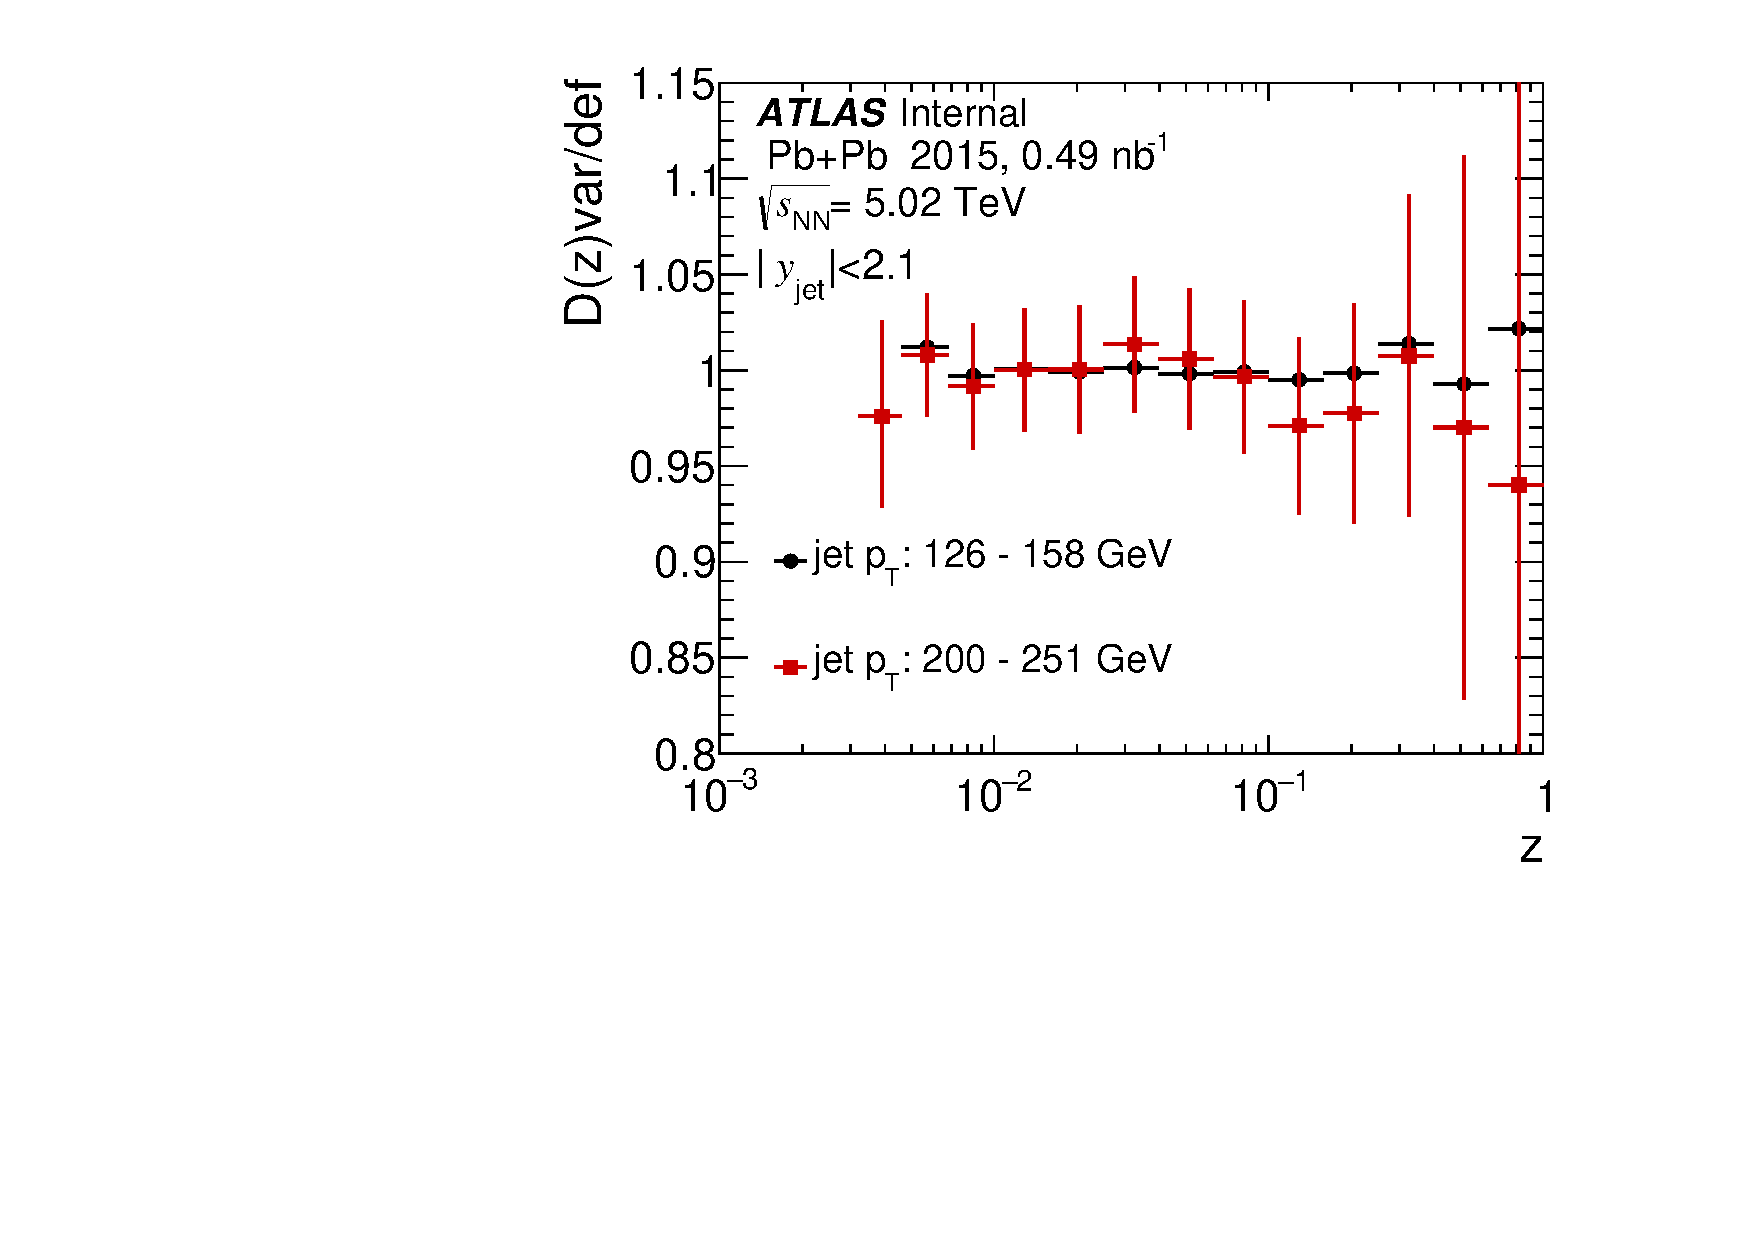
\includegraphics[width=0.45\textwidth]{figures_corrections/ff_data_comaparison_eta4_cent5_iso08.pdf} \\
%\end{tabular}}
%\caption{The ratios of the raw fragmentation functions evaluated with the more strict isolation requirement to the default version in \PbPb\ data in central (left) %and peripheral (right) collisions.}
%\label{fig:ISO80}
%\end{figure}  

%Fig.~\ref{fig:RdR} presents conditional yield of jets with $\pt^{2}$ that accompany a higher \pt\ jet with $\pt^{1}$ as a function of their angular separation $\mathrm{d}R$ in different centrality classes.
%\begin{figure}
%\centering{
%\begin{tabular}{cc}
%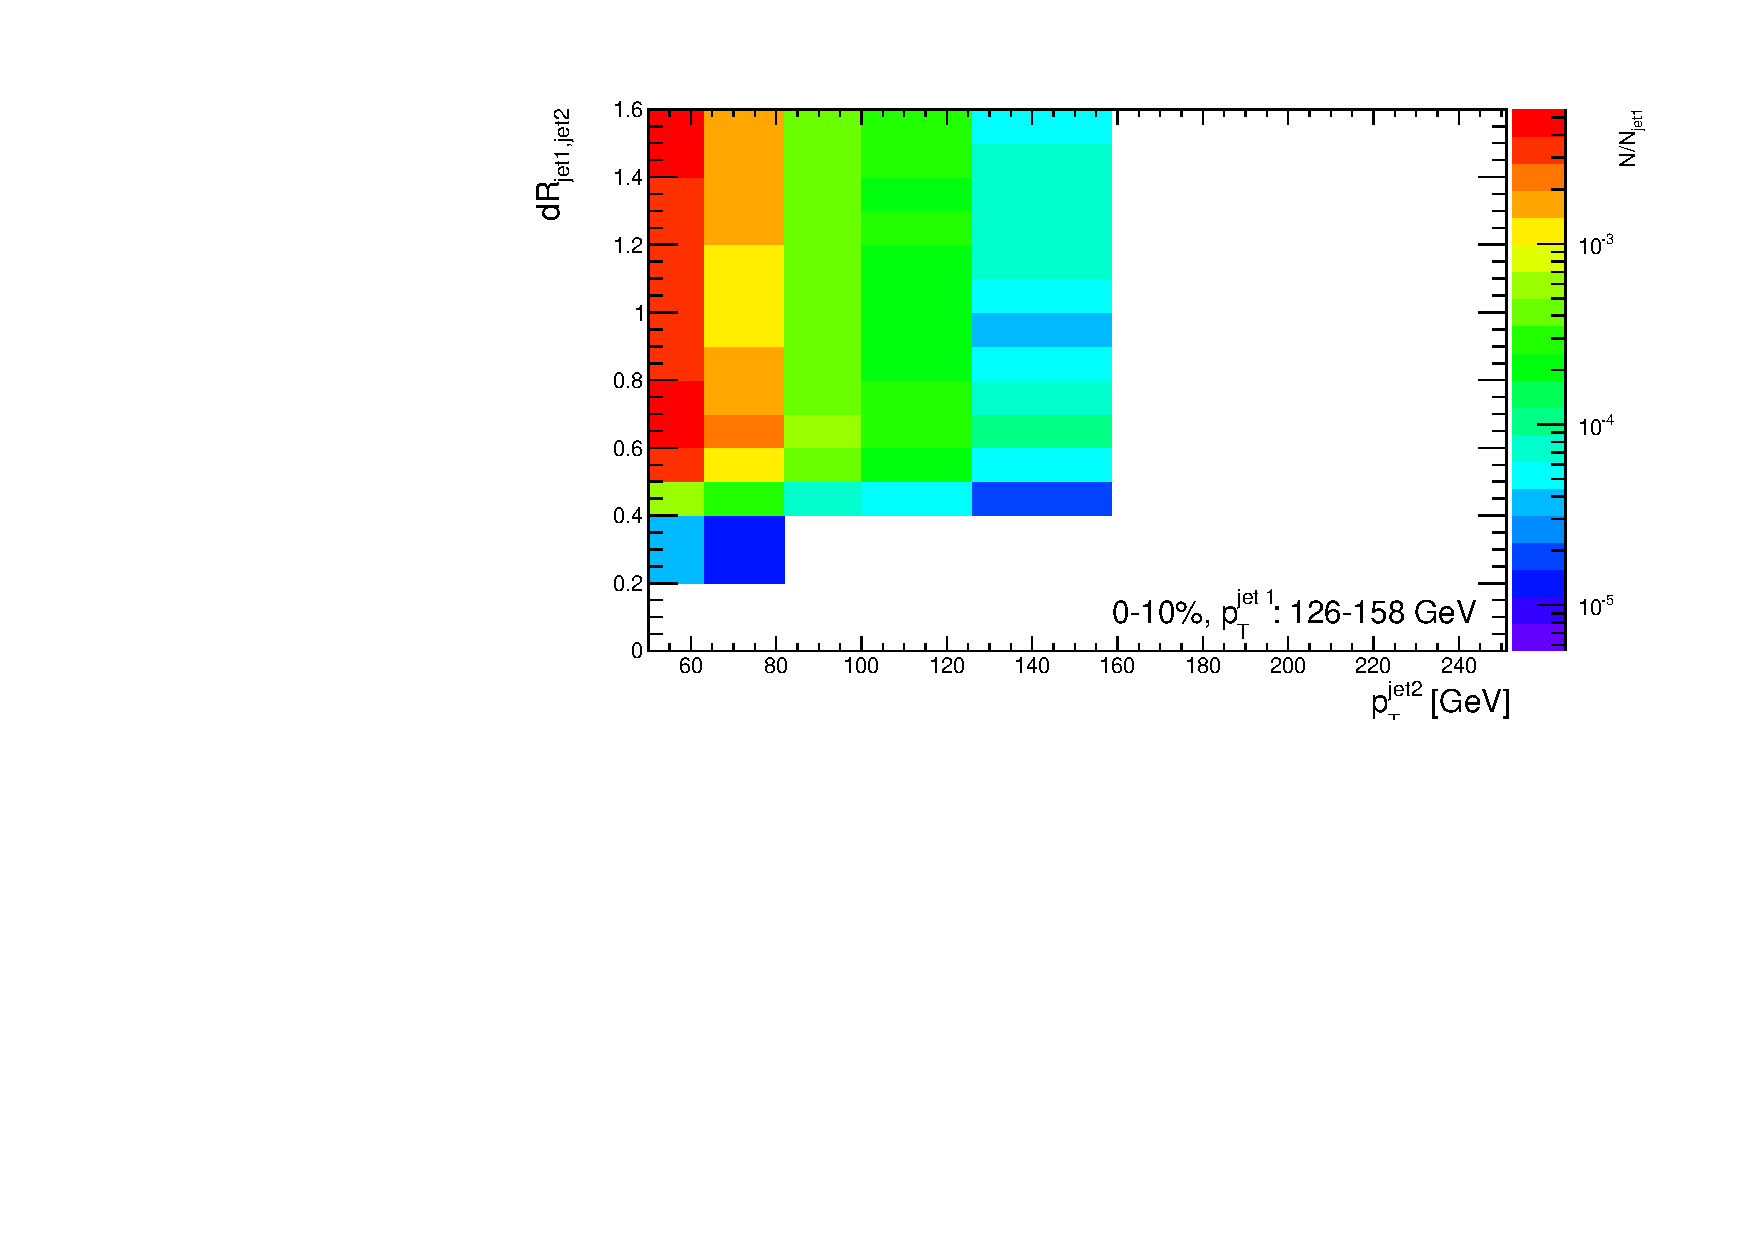
\includegraphics[width=0.45\textwidth]{figures_corrections/RdR_126_158GeV_c0.pdf} &
%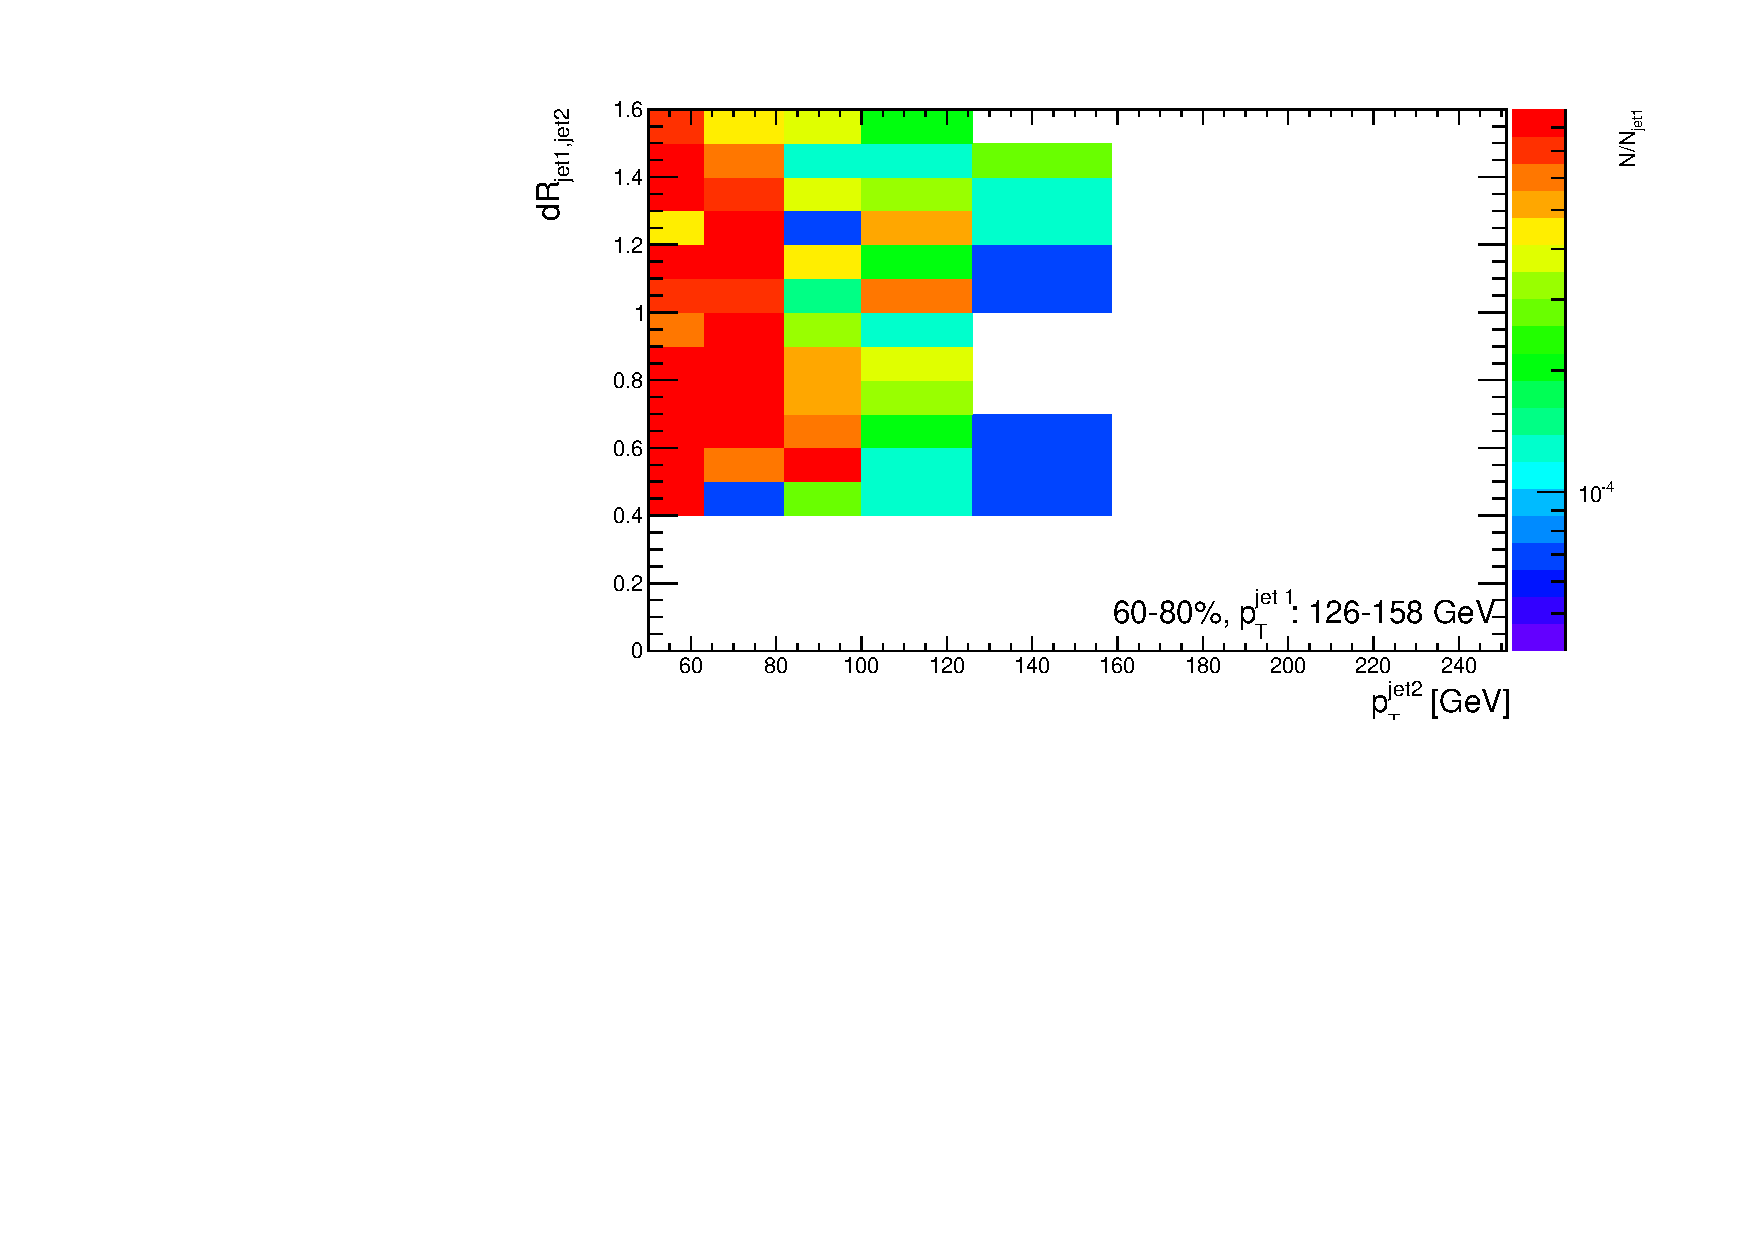
\includegraphics[width=0.45\textwidth]{figures_corrections/RdR_126_158GeV_c5.pdf} \\
%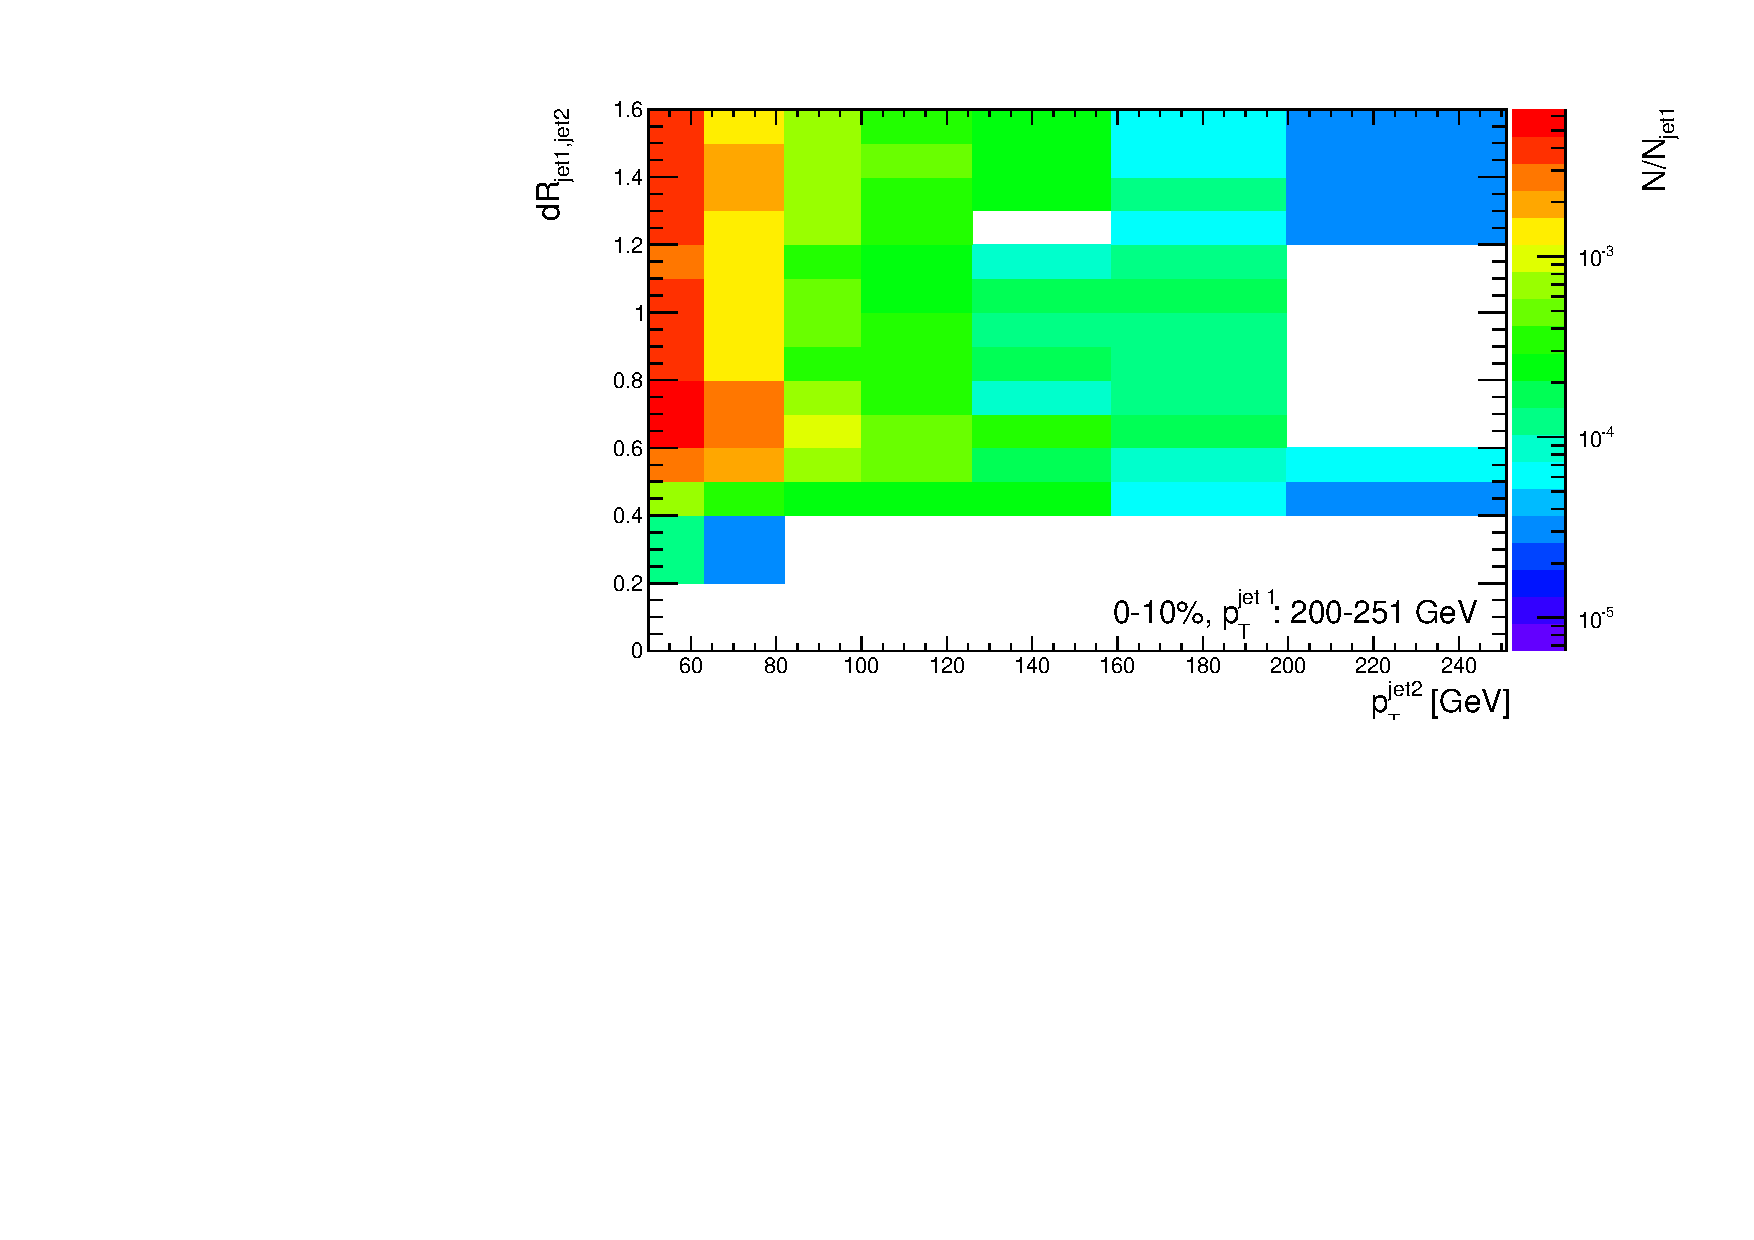
\includegraphics[width=0.45\textwidth]{figures_corrections/RdR_200_251GeV_c0.pdf} &
%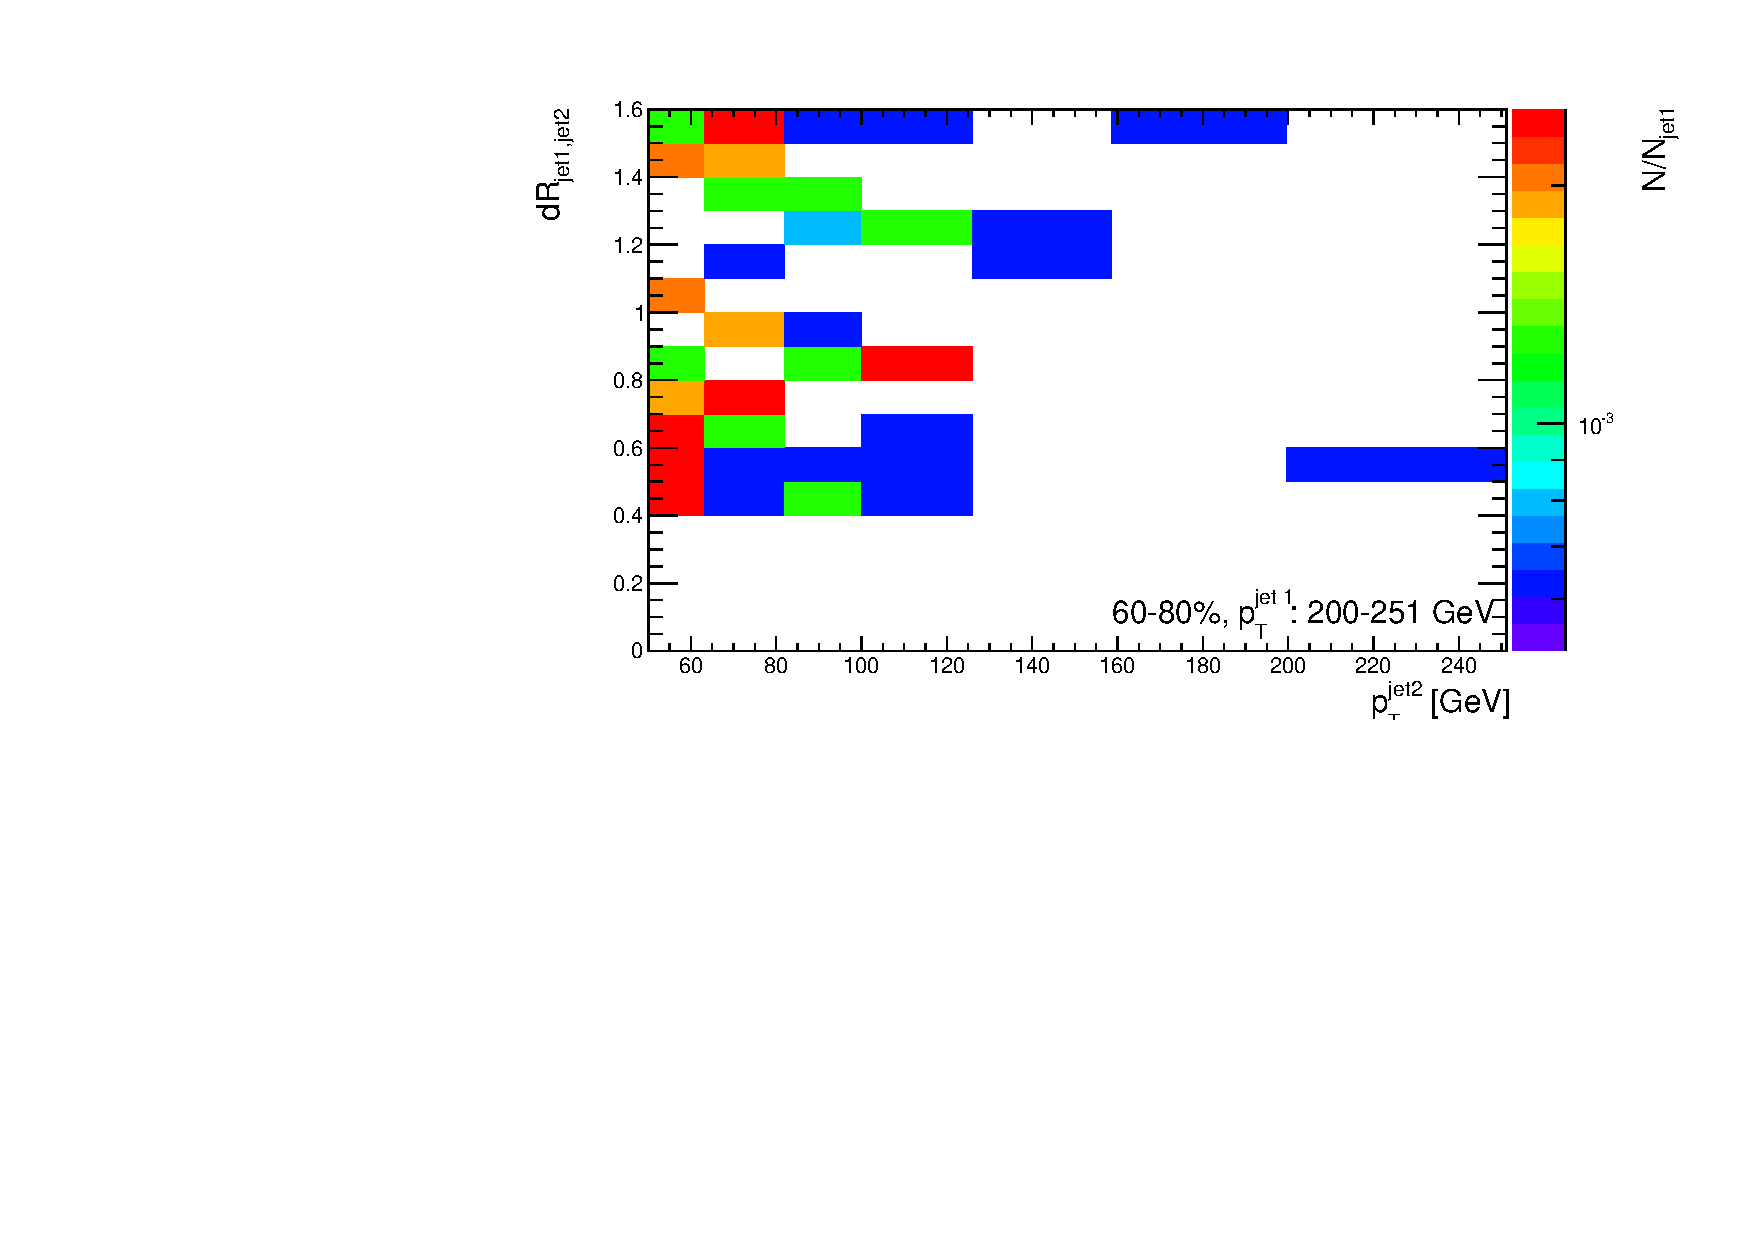
\includegraphics[width=0.45\textwidth]{figures_corrections/RdR_200_251GeV_c5.pdf} \\ 
%\end{tabular}}
%\caption{Conditional yield of jets with $\pt^{2}$ that accompany a higher \pt\ jet with $\pt^{1}$ as a function of their angular separation $\mathrm{d}R$. Distributions are presented for two different centrality bins and two different intervals of $\pt^{1}$.}
%\label{fig:RdR}
%\end{figure}  
 

\subsection{Track selection}
\label{sec:trackselection}

The track selection cuts used here follow the cuts used in~\cite{ATLAS502FFConf}. These provide a low level of fake tracks and 
a track reconstruction efficiency that is independent of the \pt\ of the jet the track is associated with.  
The cuts used here are the ``tight" cuts as described in Ref.~\cite{ref:tracktwiki} and were utilized in previous HI jet fragmentation measurements. The default tracking cuts used both in \pp\ and \PbPb\ analysis are:
\begin{itemize}
\item{ track $\pT>$~1~GeV}
\item{ track $|\eta|<$~2.5}
\item{ tracks should have at least 9 silicon hits in $|\eta|\leq1.65$}
\item{ tracks should have at least 11 silicon hits in $|\eta|>1.65$}
\item{ tracks should have at least 1 hit in IB-layer + B-layer.}
\item{tracks should have a IB-layer hit if it is expected, i.e. if the track passed an active module.}
\item{tracks should have a B-layer hit if it is expected and IB-layer hit is not expected.}
\item{ tracks should have  less than 3 holes in silicon detectors.}
\item{ tracks should have 0 holes in pixel detector.}
\item{impact parameters of track with respect to primary vertex:  $|d_0|<$$< 0.47\times \exp{(-0.15\times\pT)} + 0.19\times \exp{(0.00034\times\pT)}$~mm, $|z_0*\sin\theta|<$1.0~mm. Recommendation values are  $|d_0| < 1.5$~mm for tracks with $\pt<10$~GeV and $|d_0| < 0.2$~mm for tracks with $\pt>10$~GeV.
  	
  	This was chosen to guarantee a smooth behavior of the $d_{0}$ parameter as a function of track momentum. }
\item{ An additional cut on the track to jet \pT\ ratio is included. All tracks with 
\begin{equation}
\pTtrk >  \ptjet + \sqrt{ (3 \times \sigma_{\mathrm{JER}}(\ptjet))^2 + (3 \times \sigma_{\mathrm{TMR}}(\pTtrk))^2} 
\end{equation}
are rejected from the analysis. Where the $TMR$ stands for track momentum resolution. The purpose of this cut is to reduce the fake rate by removing tracks that have significantly larger \pt\ than the jet that they belong to.
 }
\end{itemize}

 

A tighter tracking selection is used for systematic studies (``tight+'' cuts).  These cuts include all of the default
cuts plus a 3$\sigma$ cut on the significance of the $d_0$ and $z_0 \sin\theta$.
Figures~\ref{fig:trkdataMCcomp_pp}-\ref{fig:trkdataMCcomp_pbpb_highpt}
shows comparisons of the data and MC tracking quantities in \pp\ and
\pbpb\ collisions, respectively, for different track \pT\ intervals.  Overall the MC describes the data well. A ~20\% discrepancy is observed for low impact parameters. The discrepancy is present far from the values of corresponding tracking cuts. A small overall shift of the $z0$ distribution is observed in MC samples. This difference is caused by the allowance of a small difference in the $z$ position of the primary vertex in the MC overlay procedure. However this has negligible impact on the analysis as the overall quality requirement on the pointing in the $z0$ is 1~mm. Furthermore, Fig.~\ref{fig:trkdataMCcomp_pbpb_highpt} shows the same comparison for high \pt\ tracks. All the comparisons of distributions show the same qualitative features as seen at lower \pt\ with improving pointing with increasing track \pt. The comparison of the reconstructed \pttrk\ with the generated
kinematics for tracks passing these cuts is shown in Fig.~\ref{fig:momres_pp}.

\begin{figure}
\centering{
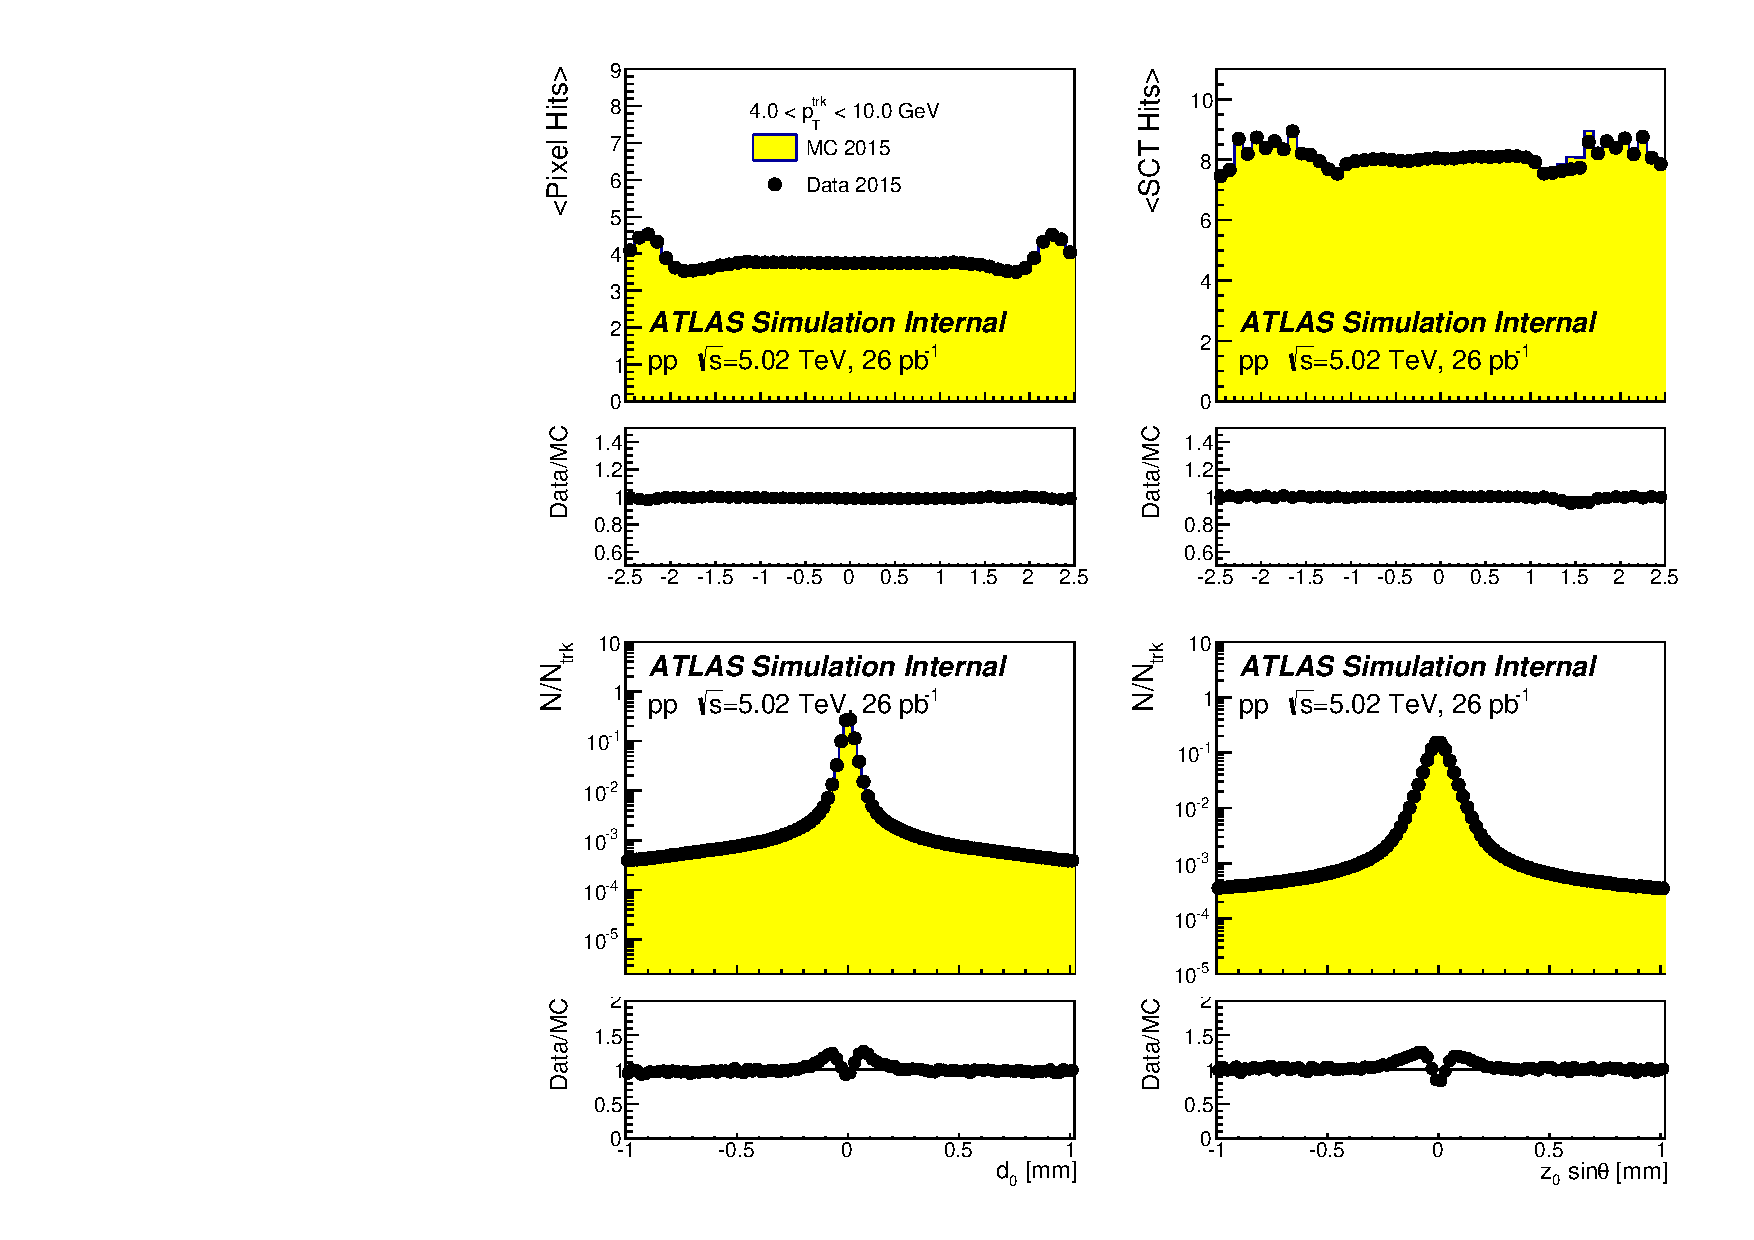
\includegraphics[width=0.75\textwidth]{figures_performance/TrkPerforPlots_5TeV_pp.pdf} }
\caption{Track quantity comparison between data (points) and MC (yellow histogram) in \pp\ collisions.  
Tracks are selected to have 4.2~$<\pttrk<$~10~GeV. Below each direct data and MC overlay is the 
corresponding data to MC ratio.  The quantities compared are: average number of pixel hits as a function
of $\etatrk$ (top left), average number of SCT hits as a function of $\etatrk$ (top right),
and number of tracks, $N_{\mathrm{trk}}$, normalized $d_0$ (bottom left), and $z_0 \sin\theta$ distributions (bottom right).}
\label{fig:trkdataMCcomp_pp}
\end{figure}

\begin{figure}
\centering{
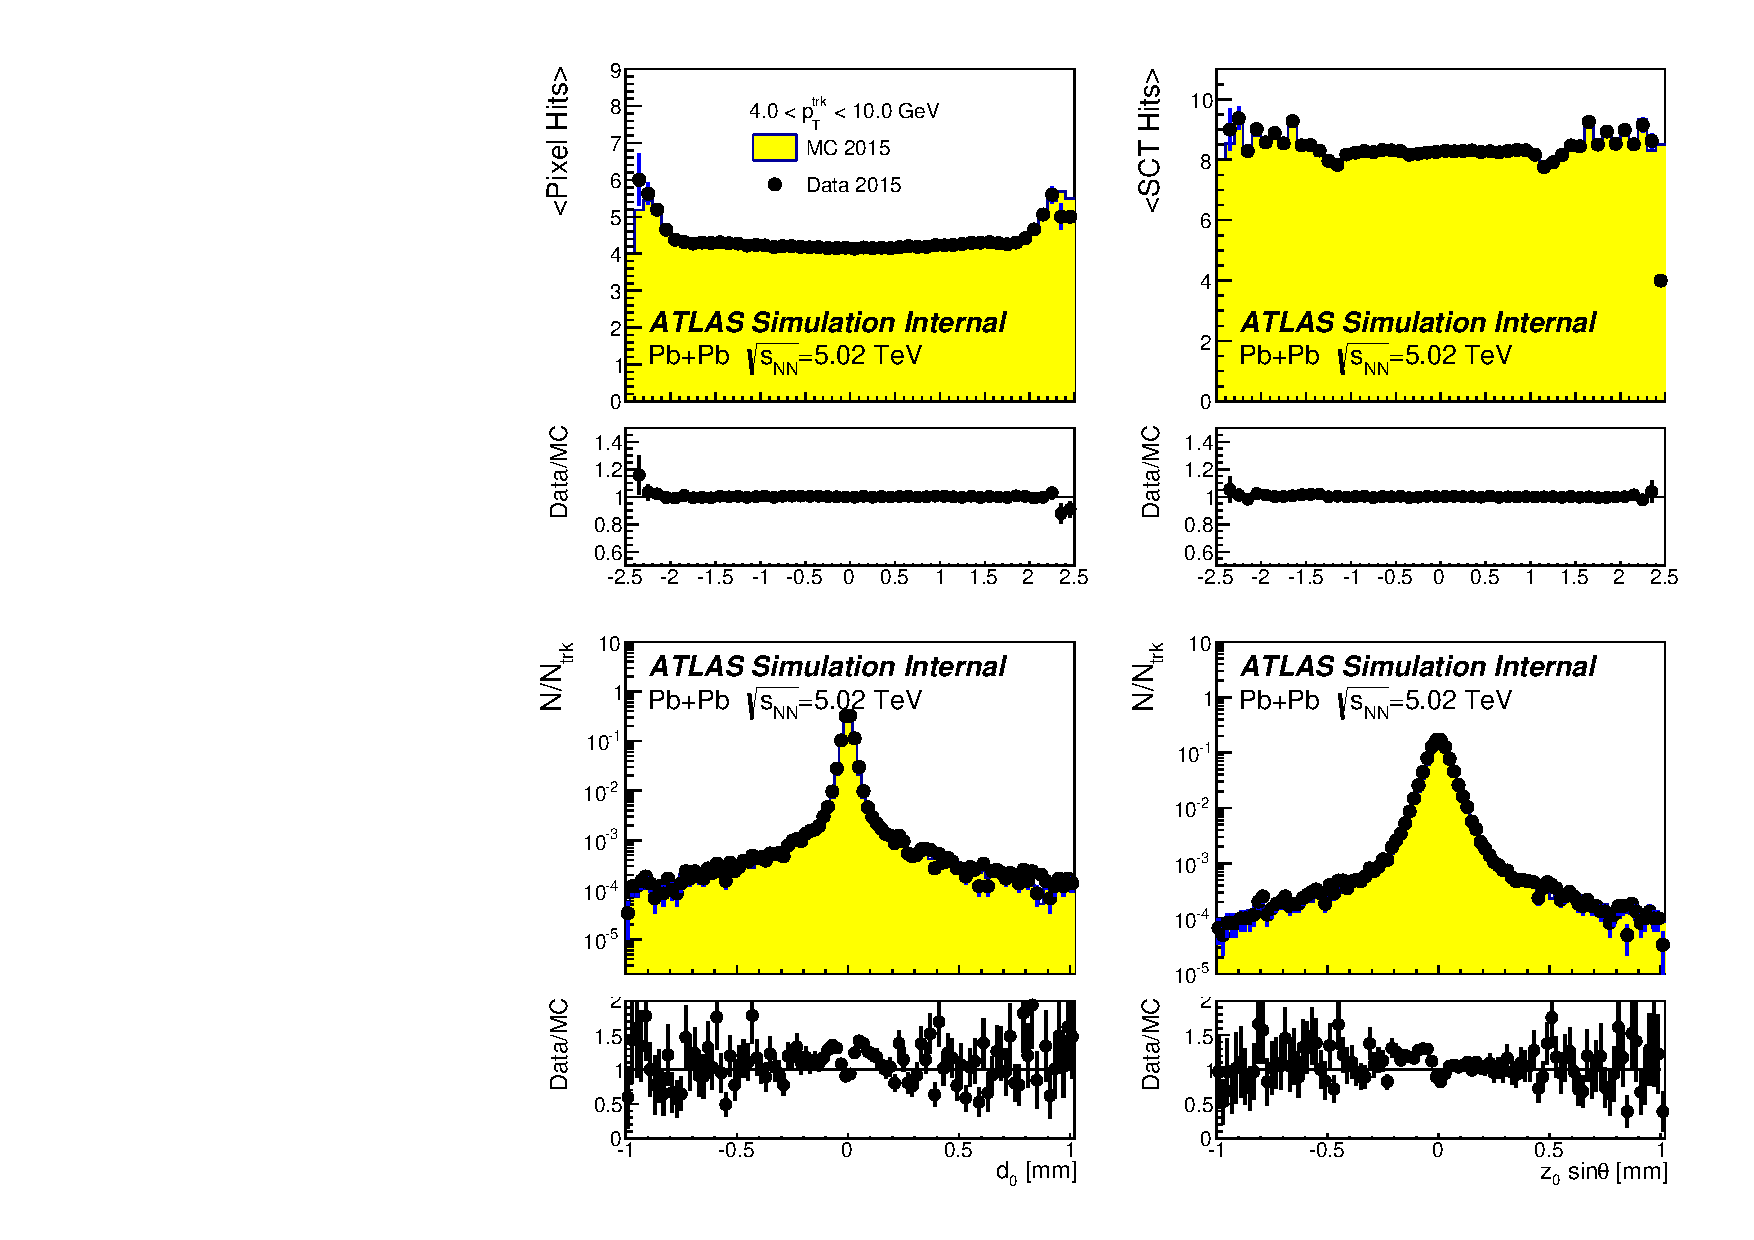
\includegraphics[width=0.75\textwidth]{figures_performance/TrkPerforPlots_PbPb_pt4p2_10p0GeV.pdf} }
\caption{Track quantity comparison between data (points) and MC (yellow histogram) in 0-10\%
   central \pbpb\ collisions.  
Tracks are selected to have 4.2~$<\pttrk<$~10~GeV. Below each direct data and MC overlay is the 
corresponding data to MC ratio.  The quantities compared are: average number of pixel hits as a function
of $\etatrk$ (top left), average number of SCT hits as a function of $\etatrk$ (top right),
track $d_0$ (bottom left), and track $z_0 \sin\theta$ (bottom right).}
\label{fig:trkdataMCcomp_pbpb}
\end{figure}

\begin{figure}
\centering{
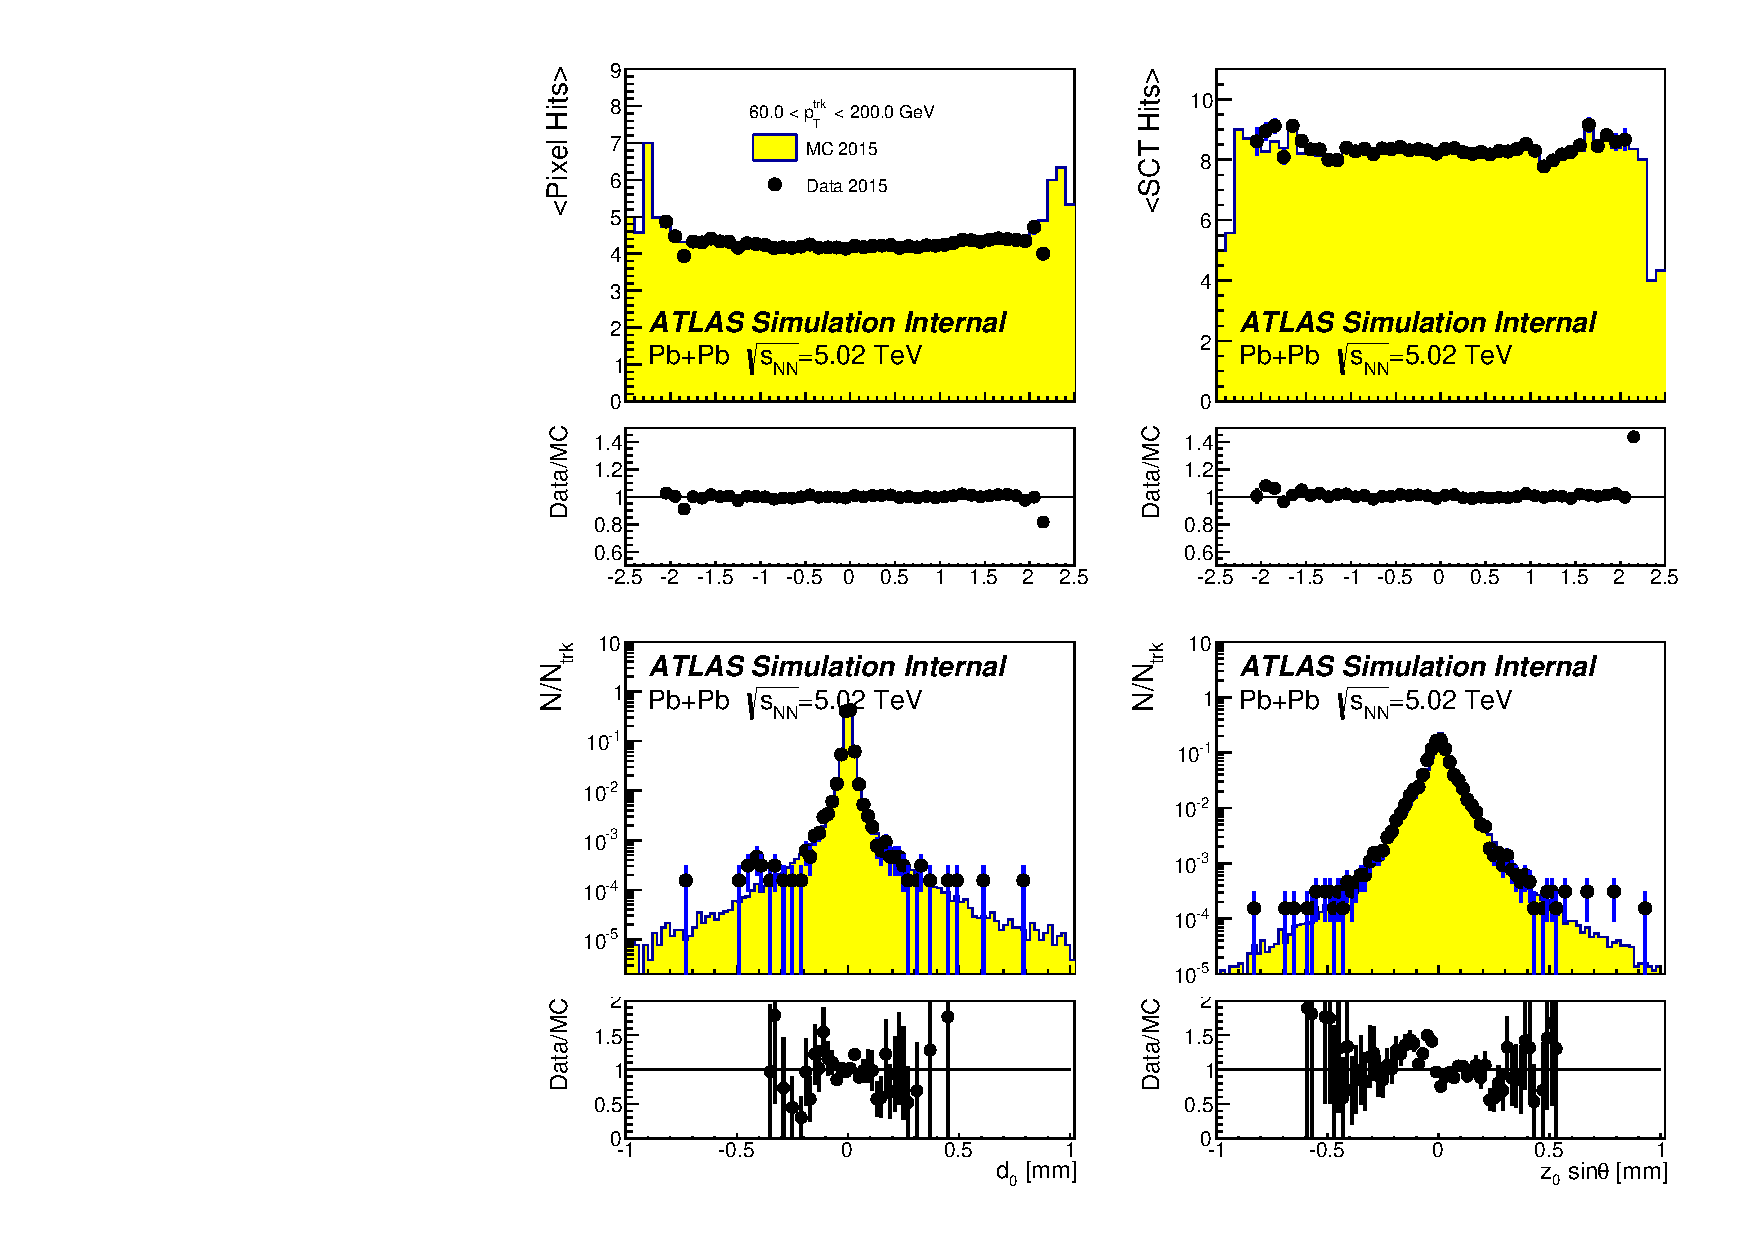
\includegraphics[width=0.75\textwidth]{figures_performance/TrkPerforPlots_PbPb_pt60_200GeV.pdf} }
\caption{Track quantity comparison between data (points) and MC (yellow histogram) in \pbpb\ collisions inclusive in collisions centrality.  
Tracks are selected to have 60~$<\pttrk<$~200~GeV and to originate from jet with \pt\ in the interval from 251 to 316 GeV. Below each direct data and MC overlay is the 
corresponding data to MC ratio.  The quantities compared are: average number of pixel hits as a function
of $\etatrk$ (top left), average number of SCT hits as a function of $\etatrk$ (top right),
track $d_0$ (bottom left), and track $z_0 \sin\theta$ (bottom right).}
\label{fig:trkdataMCcomp_pbpb_highpt}
\end{figure}


\begin{figure}
\centering{
\begin{tabular}{cc}
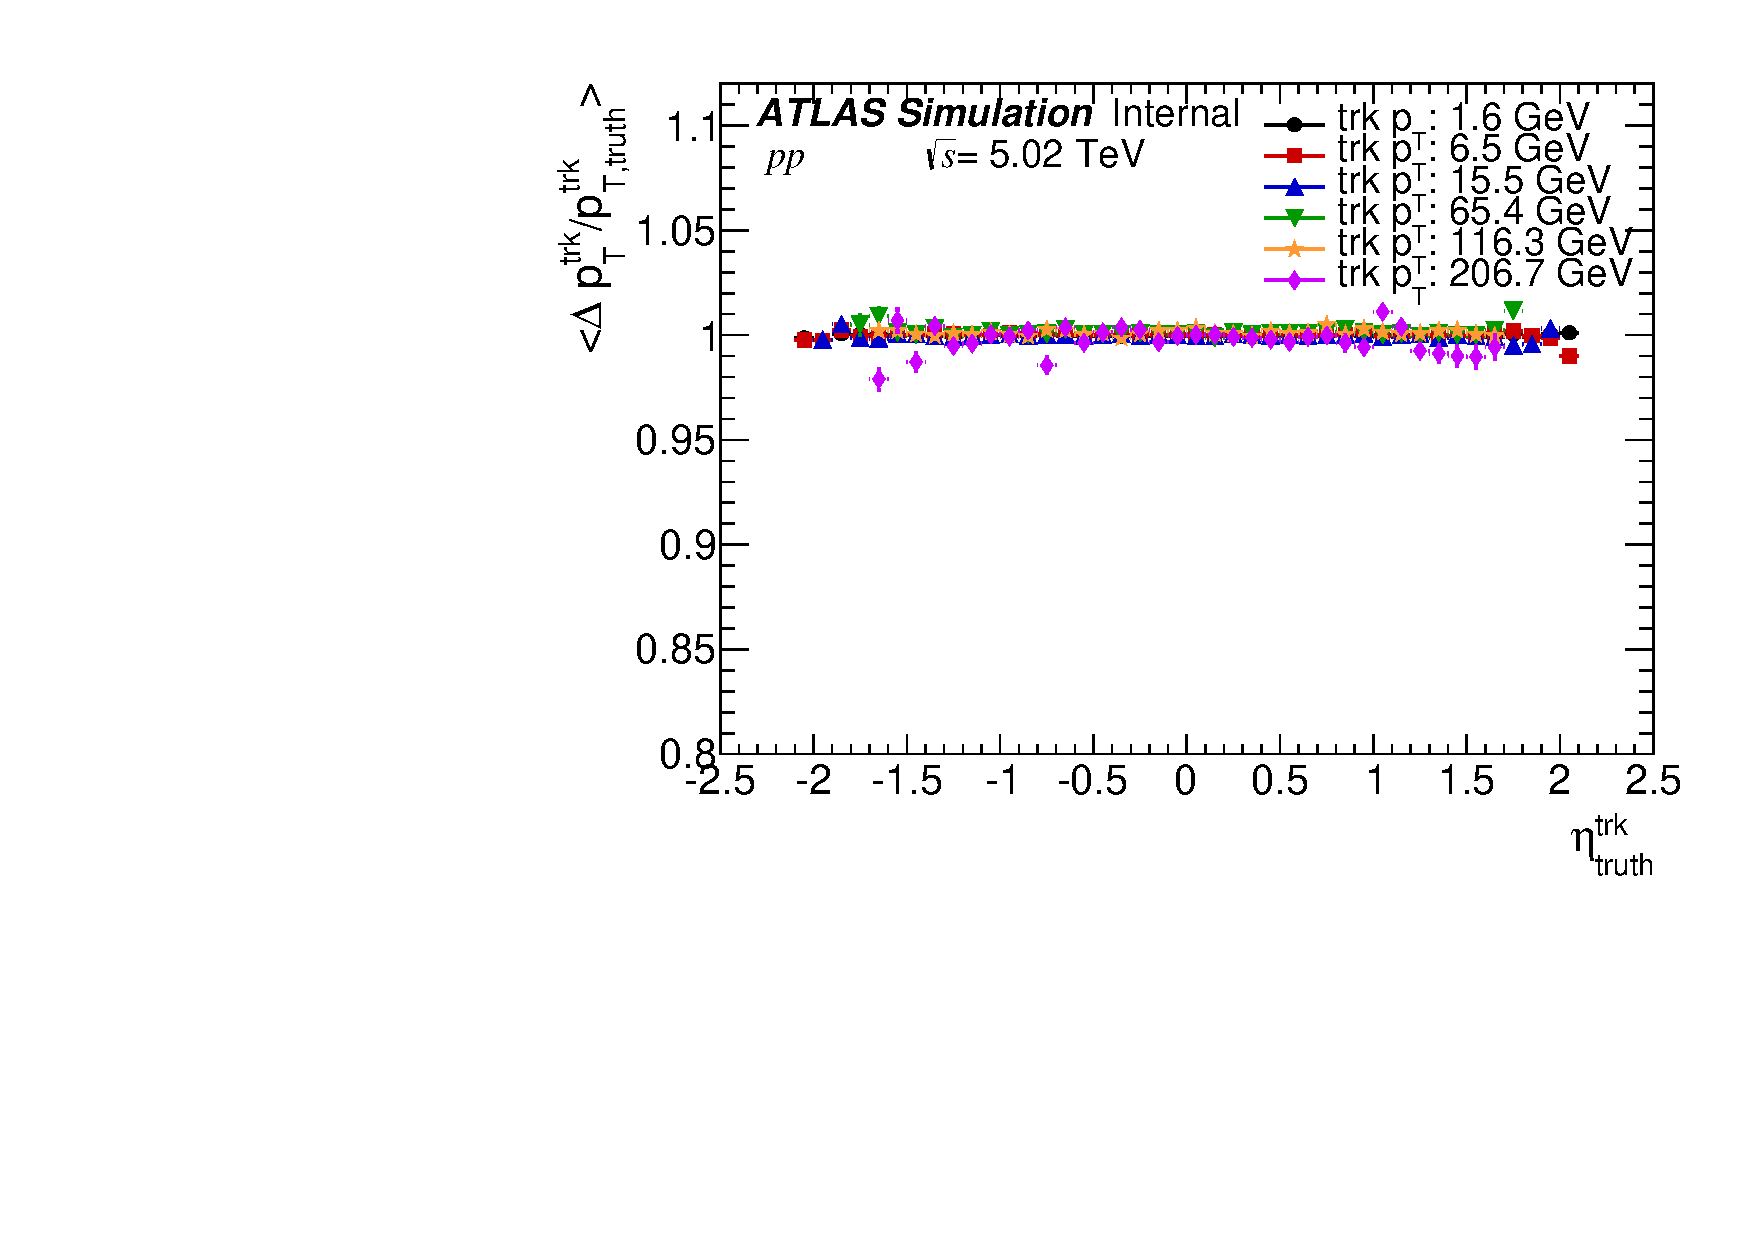
\includegraphics[width=0.45\textwidth]{figures_performance/scale_v_eta_pp.pdf} &
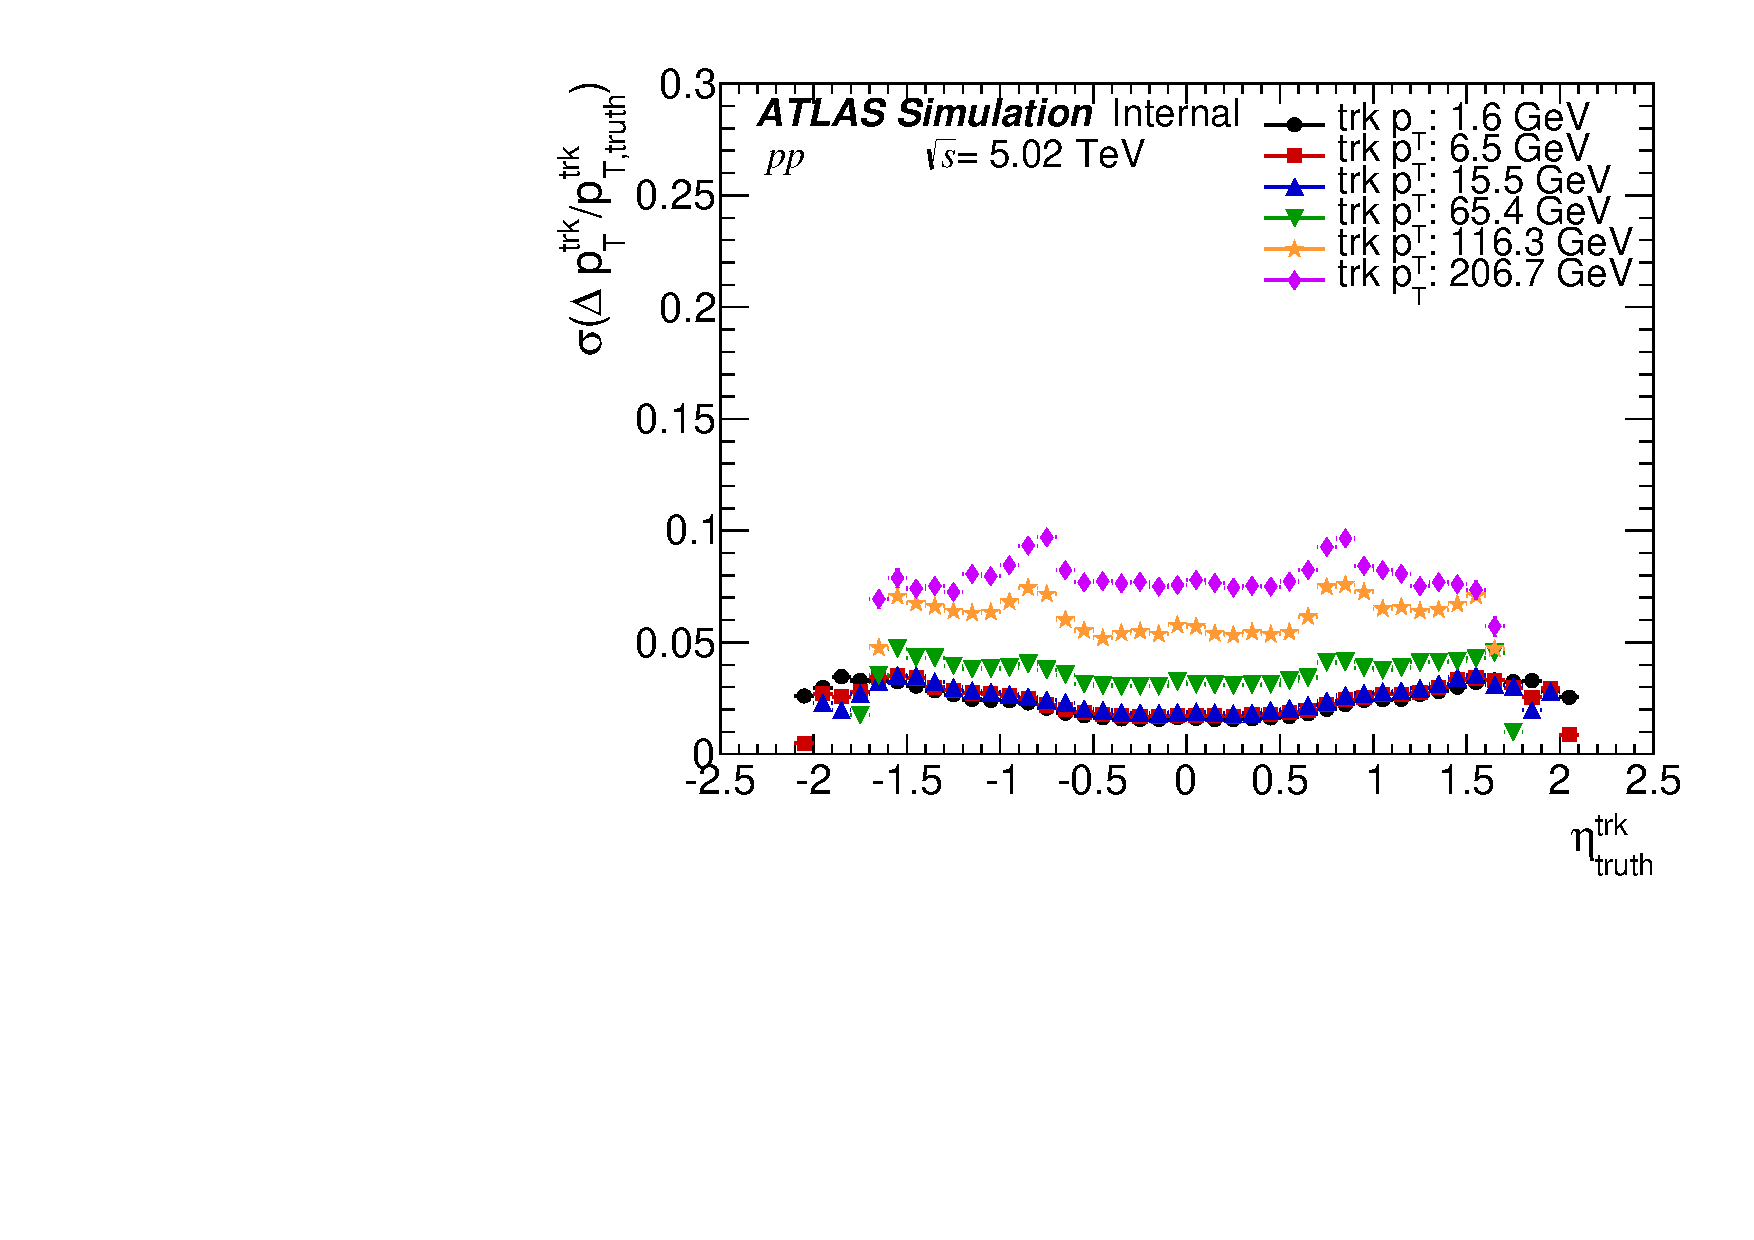
\includegraphics[width=0.45\textwidth]{figures_performance/resolution_v_eta_pp.pdf} \\ 
\end{tabular}}
\caption{(left) Comparison of the generated and reconstructed track \pt\ as a function of \etatrktruth\ for 
five track \pttrktruth\ selections. 
(right) Track momentum resolution as a function of \etatrktruth\ for five \pttrktruth\ selections.
Both plots are for \pp\ MC.  
All tracks shown in this plot have passed the 2015 default tracking cuts defined in this section.}
\label{fig:momres_pp}
\end{figure}



Figure~\ref{fig:ppcutflow_eta} presents the impact of individual tracking requirements in terms of the ratio of the number of tracks that pass given cut and the total number of reconstructed tracks in \pp\ MC. The study is presented as a function of track pseudorapidity in two different track \pT\ intervals and as a function of track \pT\ in two different pseudorapidity intervals. The highest rejection for low \pT\ tracks is provided by the cut on $d_{0}$ pointing. At high \pT\, the dominant effect is seen from the requirement on the number of silicon hits. Similarly, Fig.~\ref{fig:PbPbcutflow_eta} presents the impact of individual tracking requirements in \PbPb\ MC. The difference between the impact of individual cuts can be attributed to a different setting of the tracking algorithm and to the overall increase of the track multiplicity as the number of rejected tracks does not linearly scale with the multiplicity that enters the denominator.       

\begin{figure}
\centering{
\begin{tabular}{cc}
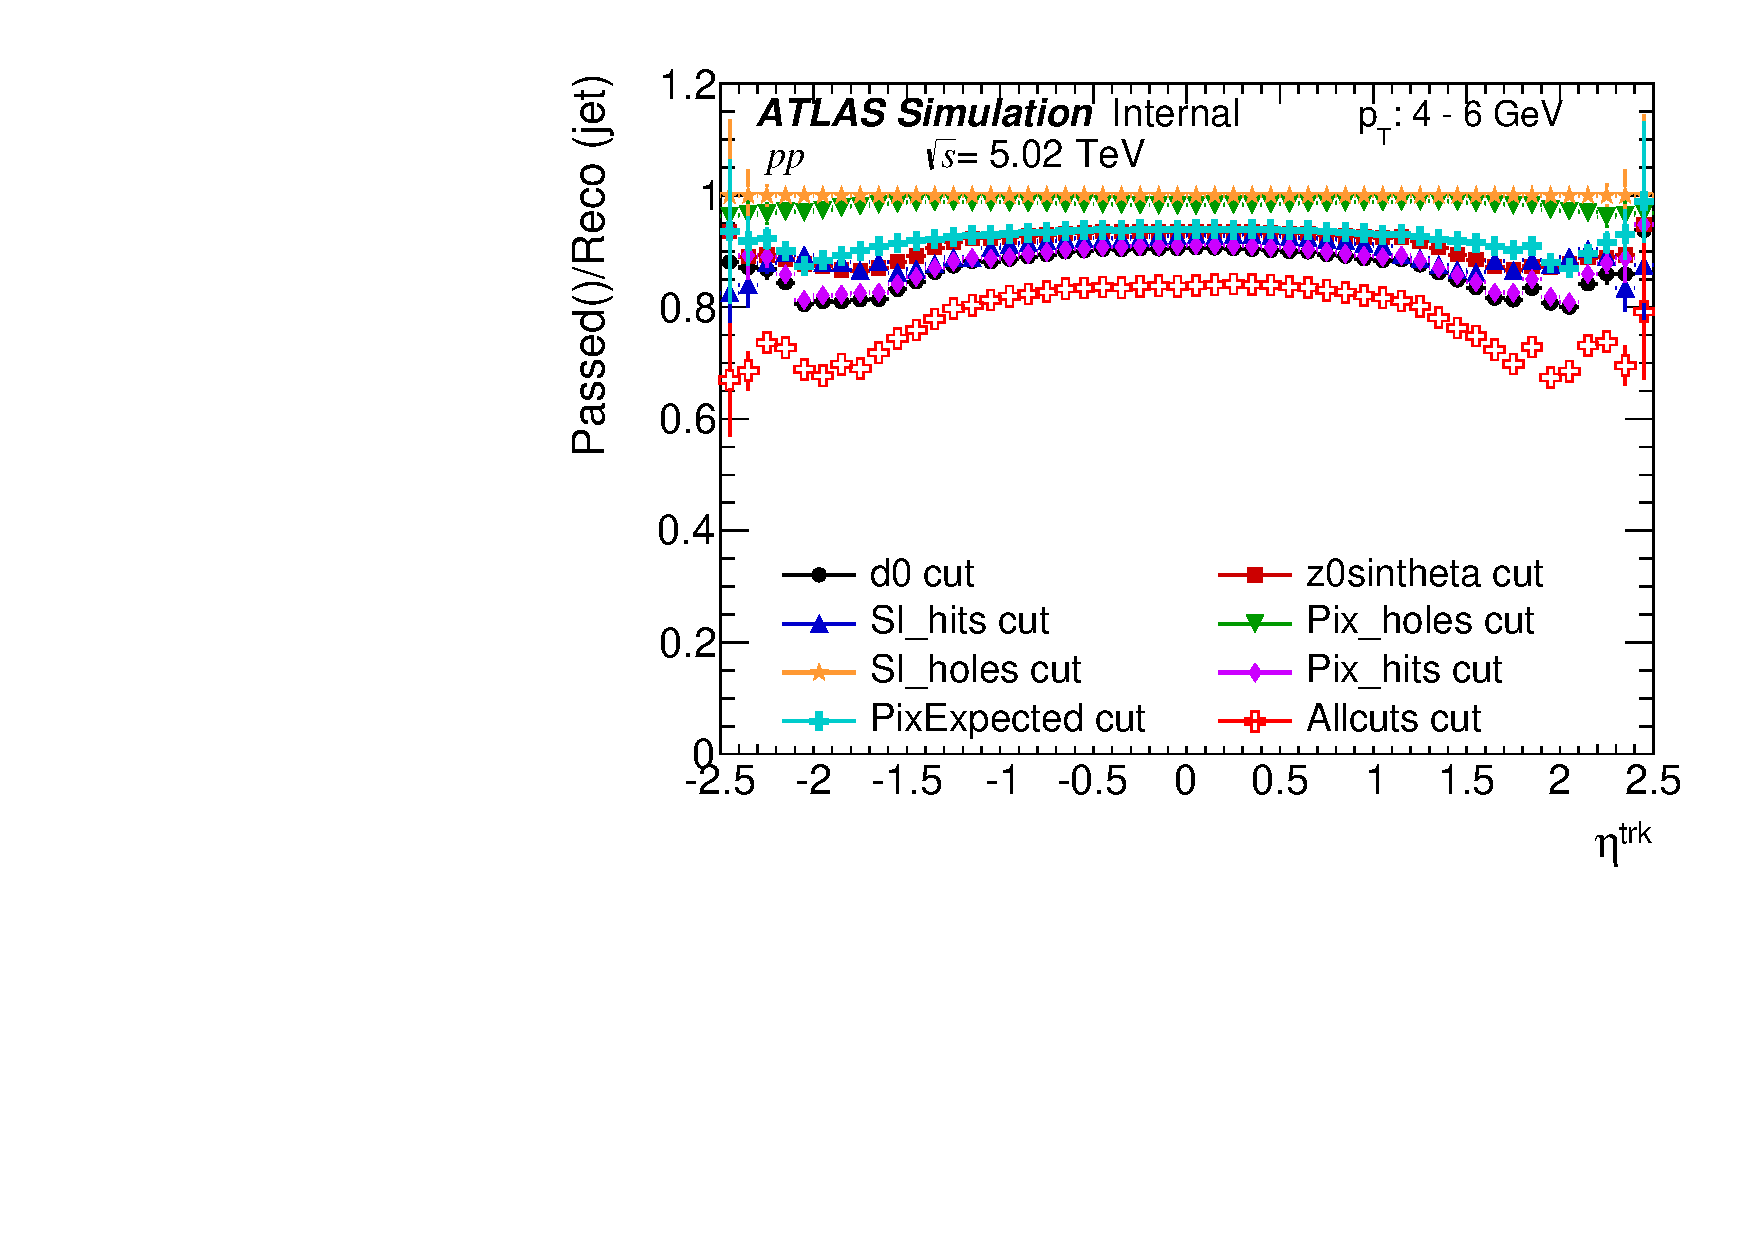
\includegraphics[width=0.45\textwidth]{figures_performance/cut_flow_RecoNorm_MC_pT_4_6_jet.pdf} &
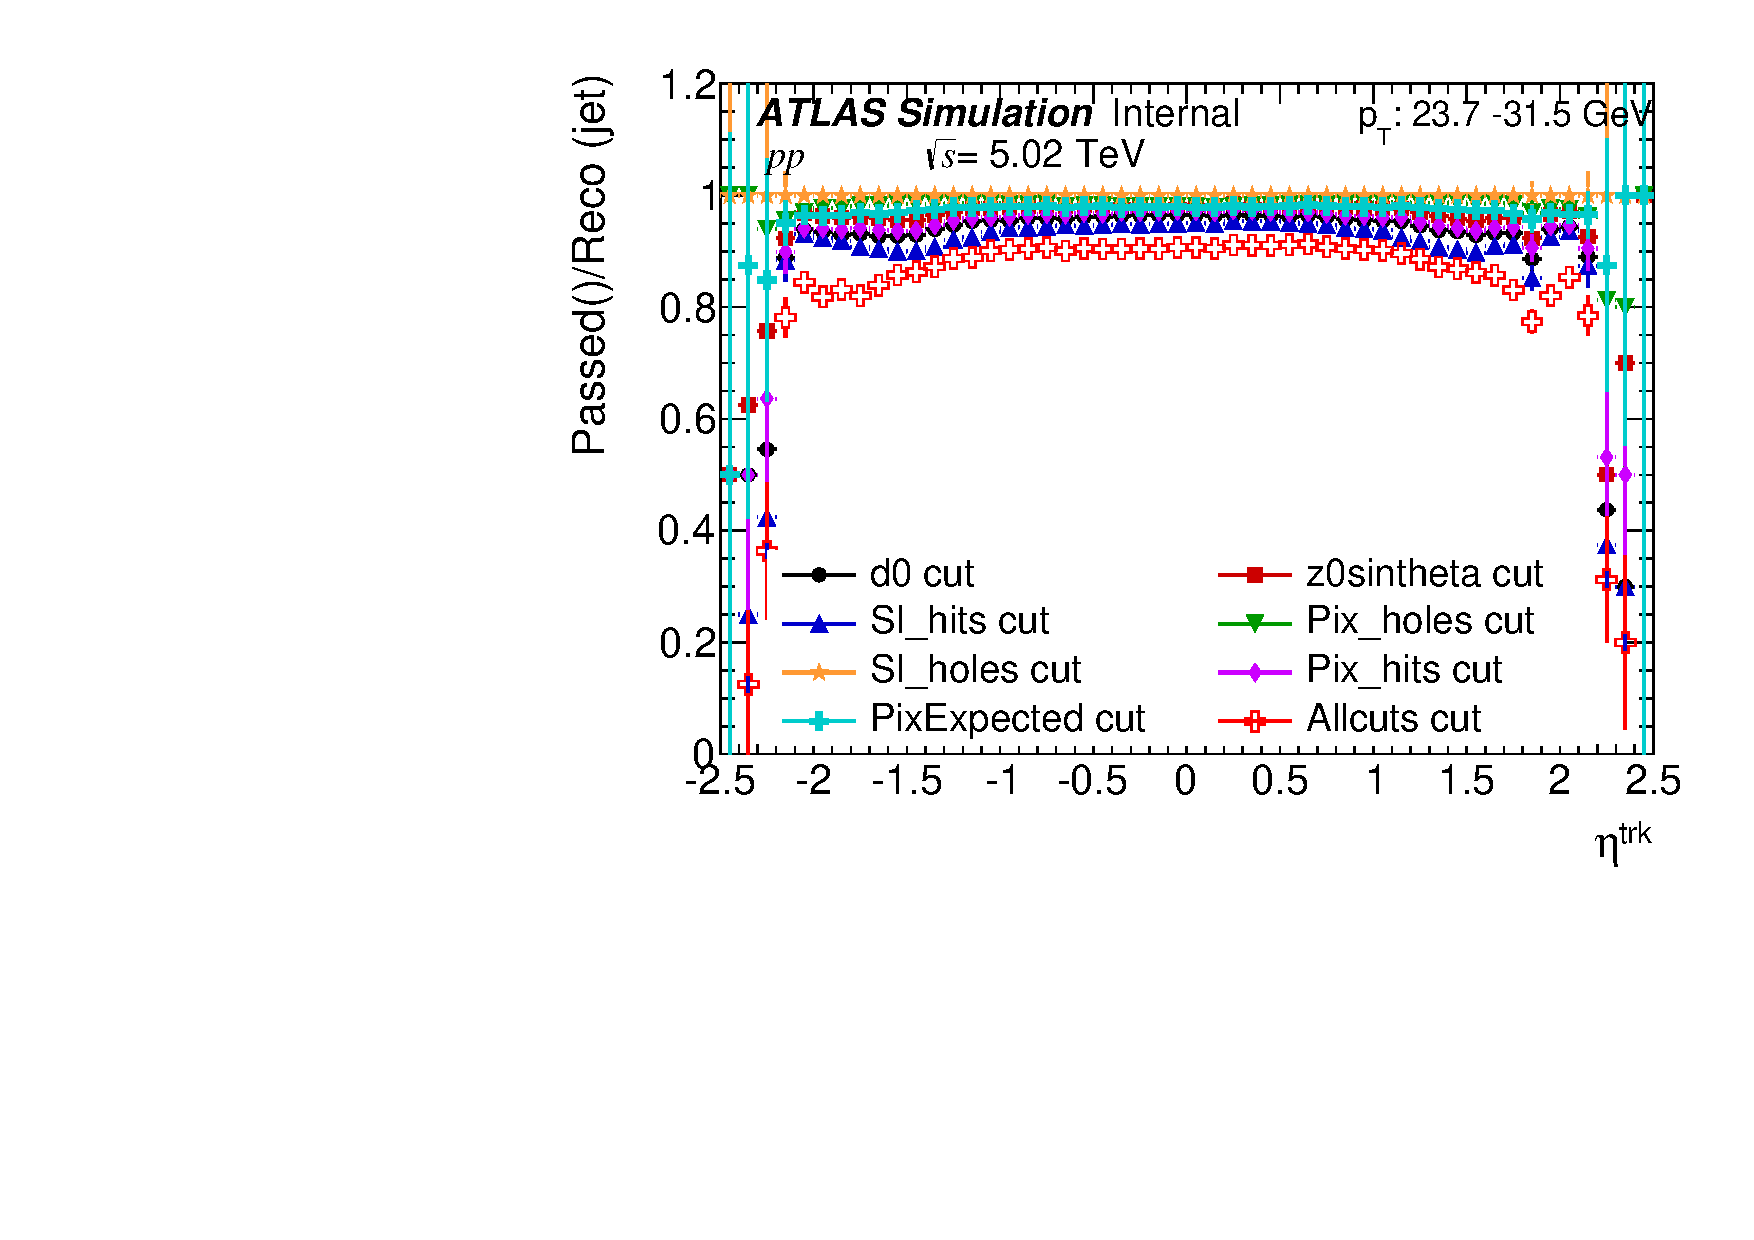
\includegraphics[width=0.45\textwidth]{figures_performance/cut_flow_RecoNorm_MC_pT_23p7_31p5_jet.pdf} \\
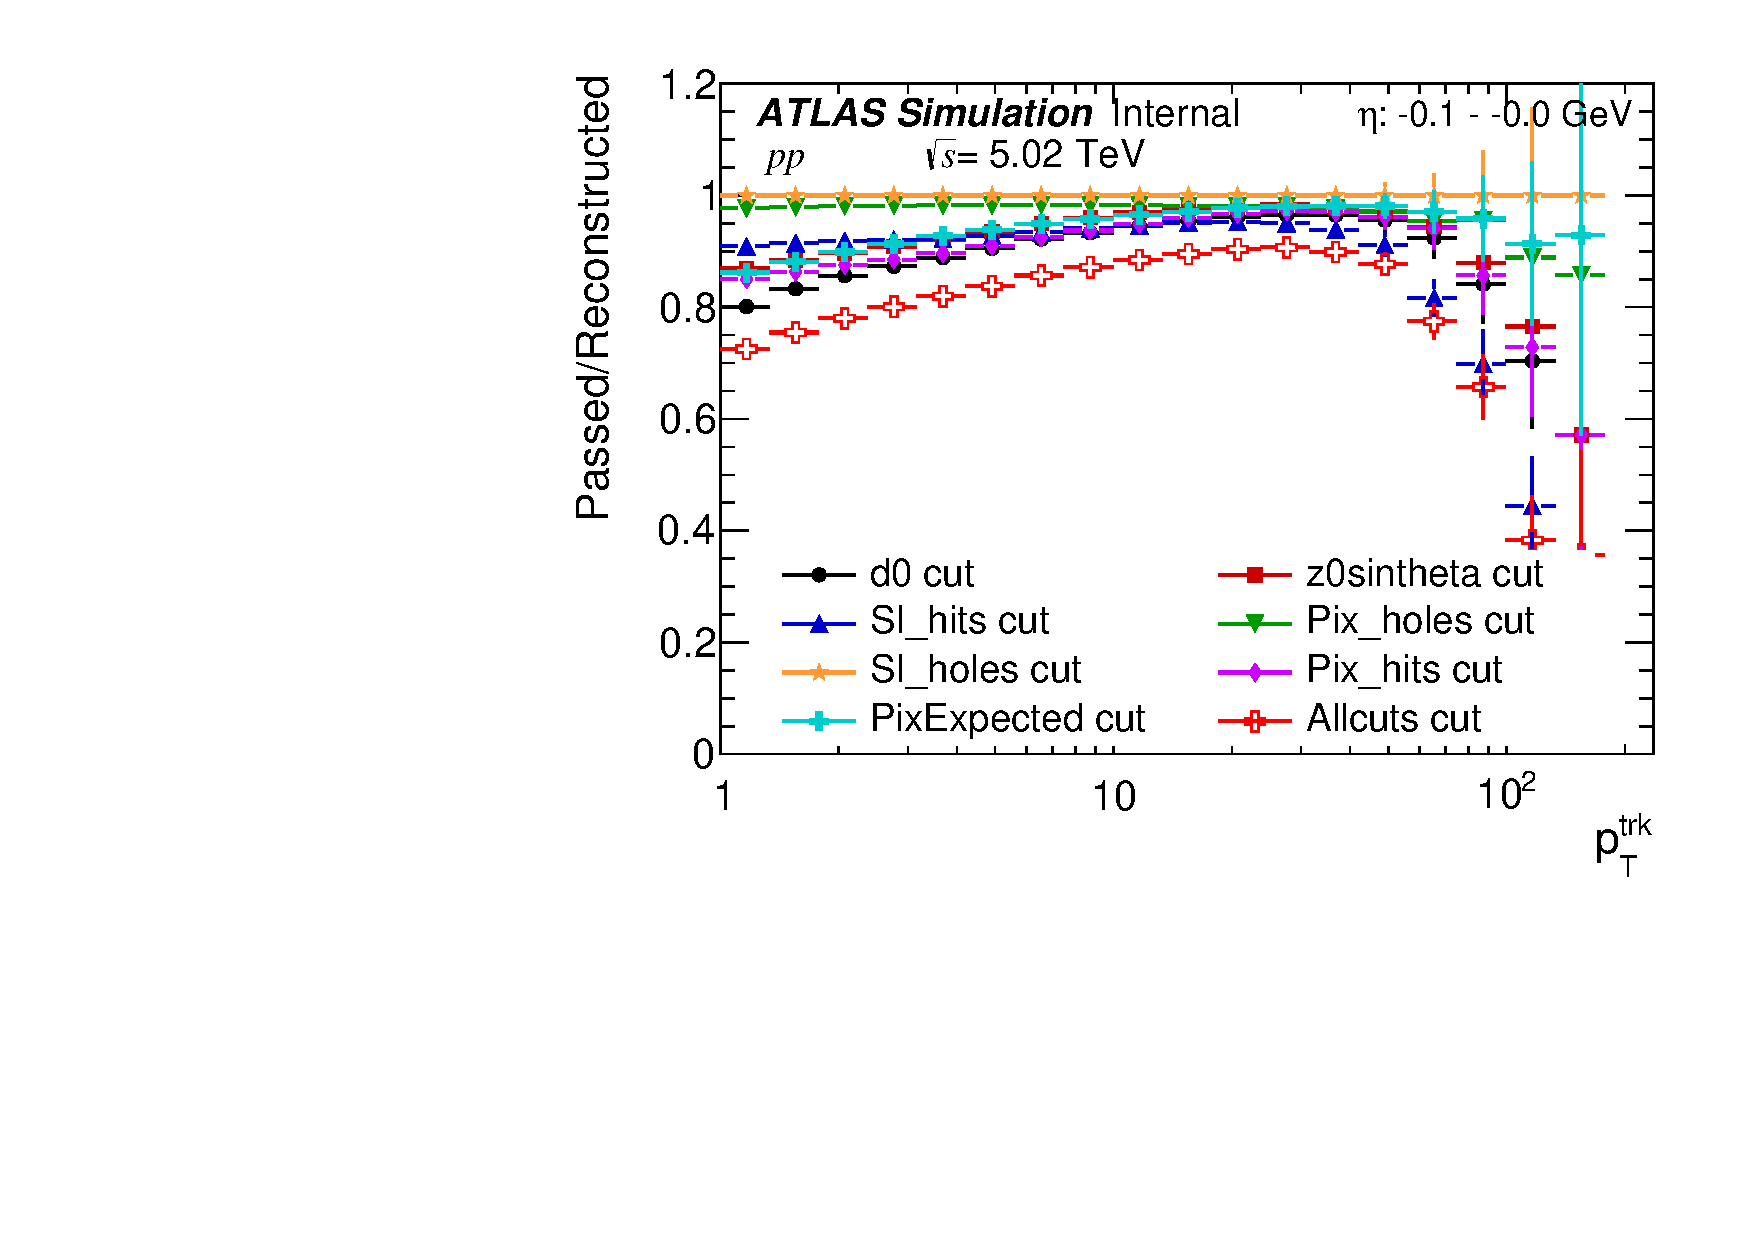
\includegraphics[width=0.45\textwidth]{figures_performance/cut_flow_RecoNorm_MC_eta_0p05_jet.pdf} &
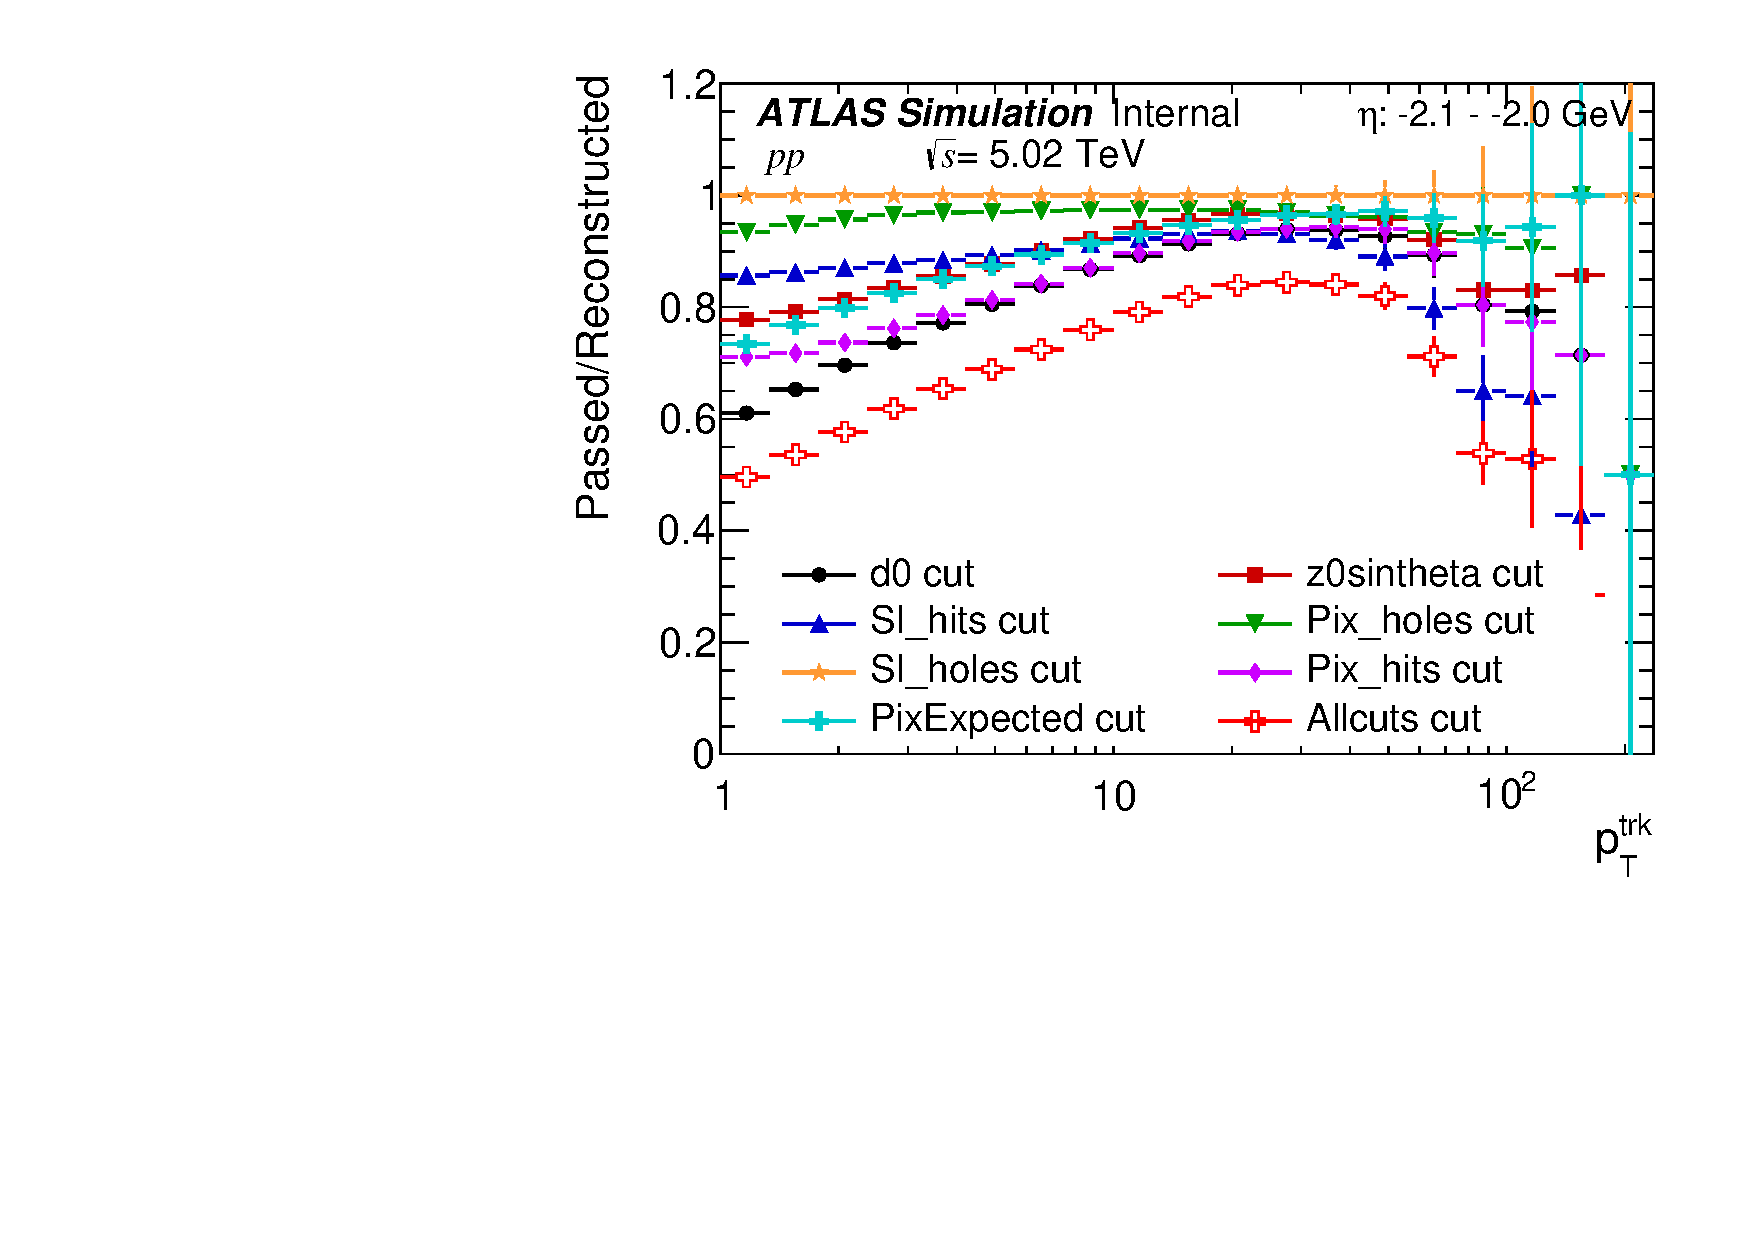
\includegraphics[width=0.45\textwidth]{figures_performance/cut_flow_RecoNorm_MC_eta_2p05_jet.pdf} \\
\end{tabular} }
\caption{The impact of each cut applied individually in the \pp\ MC 
to the starting collection of tracks, as a function of
\etatrk (top) for 4.6~$>\pttrk>$~1.3~GeV (left) and for 23.7~$<\pttrk<$~31.5~GeV and as a function of track \pT\ for two different pseudorapidity intervals (bottom).  The final combination of all cuts is shown as well.}
\label{fig:ppcutflow_eta}
\end{figure}

\begin{figure}
\centering{
\begin{tabular}{cc}
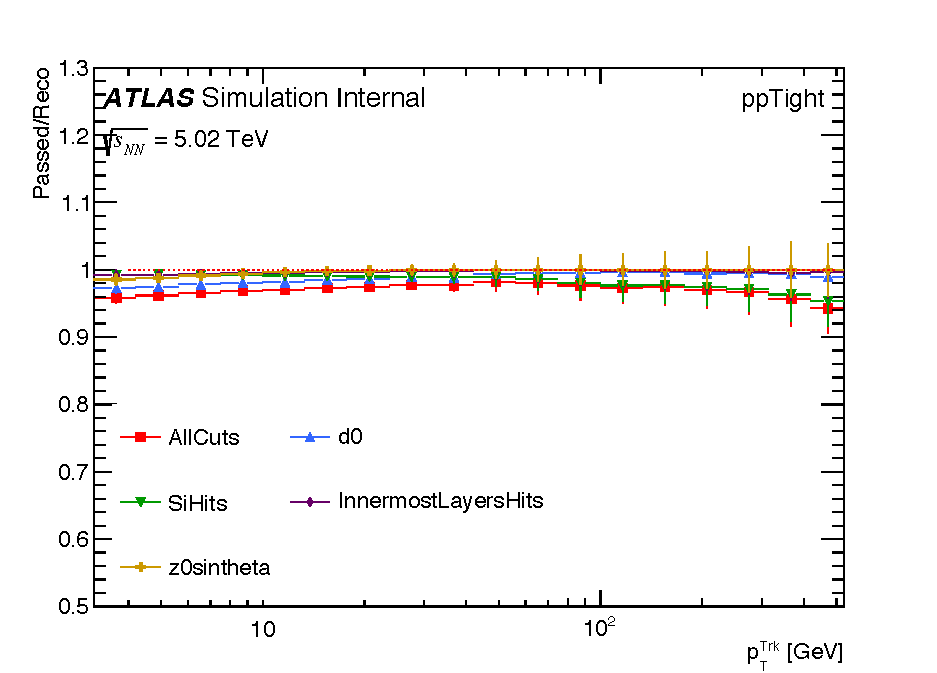
\includegraphics[width=0.45\textwidth]{figures_performance/PbPb_cutflow_pptight.pdf} &
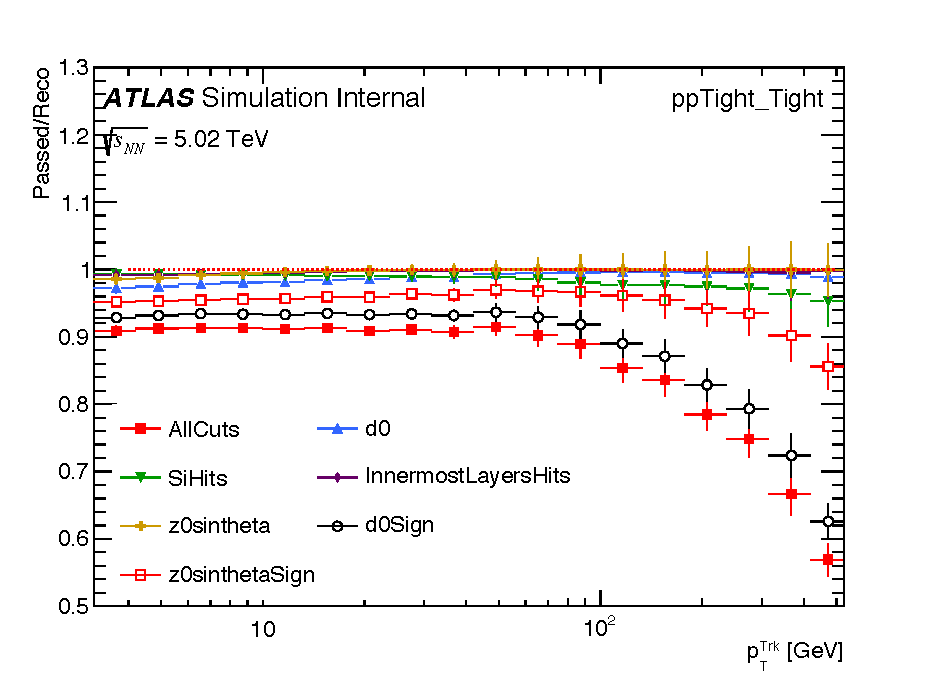
\includegraphics[width=0.45\textwidth]{figures_performance/PbPb_cutflow_pptight_tight.pdf} \\
\end{tabular} }
\caption{The impact of each cut applied individually in the \PbPb\ MC 
to the starting collection of tracks, as a function of the track \pT\ inclusive in collision centrality for the default and the tight set of tracking requirements. The final combination of all cuts
is shown as well.}
\label{fig:PbPbcutflow_eta}
\end{figure}

\subsection{Track momentum correction}
\label{Sec:Trackmomentumcorrection}
Specific correction is needed for track momentum in 5~TeV \pp\ and \PbPb\ data to account for miss-alignment introduced in the track reconstruction. The sign charge dependent momentum scale shift was observed in \pp\ data when the transverse momentum of muons reconstructed using muon spectrometer was compared to the transverse momentum of muons from the inner detector. The difference as a function of muon momentum can be seen in Fig.\ref{Fig:ChMomentumScale}. The correction to track \pt\ as a function of track $\eta$ and track $\phi$ is applied through sagitta bias maps introduced in InDetTrackSystematicsTools-00-00-19~\cite{TrackingRec}.

\begin{figure}[h]
\centerline{
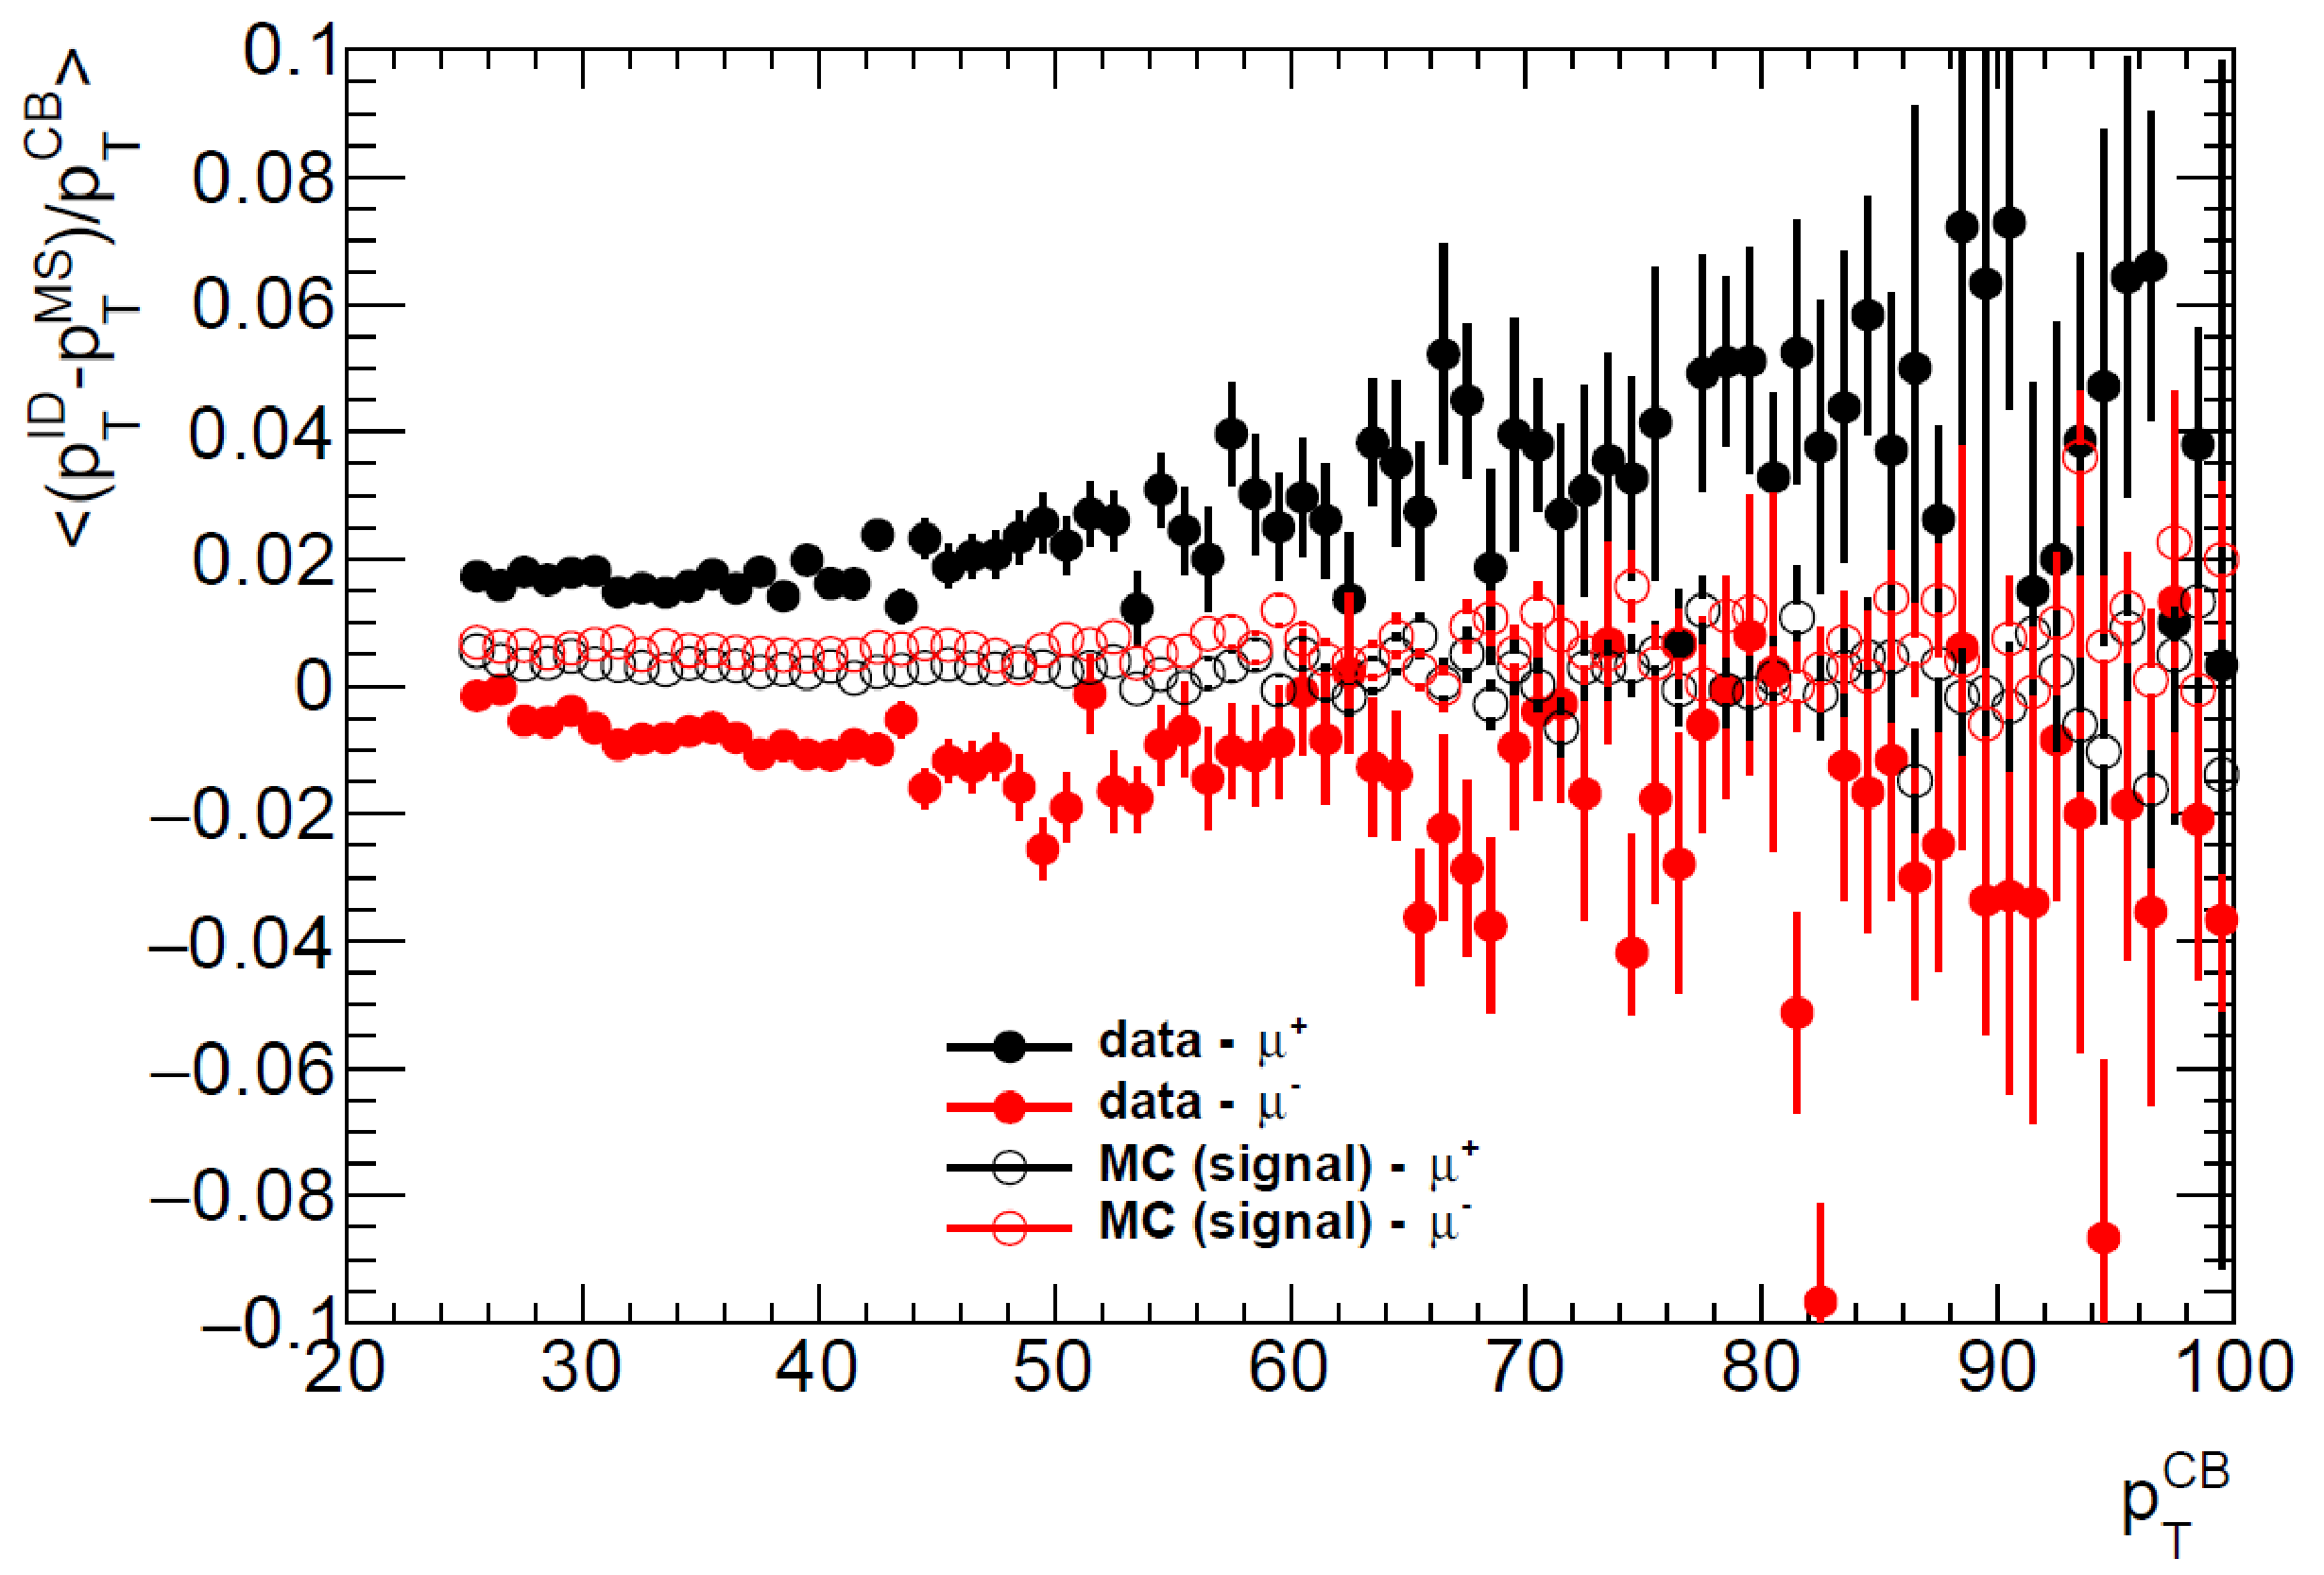
\includegraphics[width=0.75\textwidth]{figures_corrections/MuonPerf.pdf}
}
\caption{Comparisons of track momentum scale of positive and negative muons reconstructed using muon spectrometer and inner detector. The muon traverse momentum evaluated from muon spectrometer (MC) is compared by that evaluated using the inner detector (ID) and the relative scale is normalized by the momentum that uses both detectors (CB). \cite{Bold:2194917}}
\label{Fig:ChMomentumScale}
\end{figure}

%\clearpage


\subsection{Track reconstruction efficiency}
\label{sec:trackreco}

The track reconstruction efficiencies are evaluated by using MC tracks. The tracking reconstruction efficiency is defined as the ratio between the number of primary truth charged particles that are reconstructed and the total number of primary truth charged particles in the given \pt\ and $\eta$ bin. Primary particles are defined as particles with a mean lifetime $\tau > 0.3 \times 10^{-10}$~s either directly produced in \pp\ interactions or
from subsequent decays of particles with a shorter lifetime. All other particles are considered to be secondary.  Tracks are required to pass all the tracking cuts imposed on the data. 

Matching between the reconstructed and the truth track is done via a cut on $mc_{\mathrm{prob}}$. The $mc_{\mathrm{prob}}$ variable is calculated according to:
\begin{equation}
mc_{\mathrm{prob}} = \frac{10N^{\mathrm{common}}_{\mathrm{pix}} + 5N^{\mathrm{common}}_{\mathrm{SCT}} + N^{\mathrm{common}}_{\mathrm{TRT}}}{10N^{\mathrm{track}}_{\mathrm{pix}} + 5 N^{\mathrm{track}}_{\mathrm{SCT}} + N^{\mathrm{track}}_{\mathrm{TRT}}
\label{eq:mc_prob}}
\end{equation}
 where $N^{\mathrm{common}}_X$  are the number of hits in detector $X$ in common between the truth and reconstructed track.  $N^{\mathrm{track}}_X$ is the number
of total hits in the reconstructed track.  
Tracks with a $mc_{prob}$ greater than 0.3 are associated with the truth track and those with a lower value are not and are classified as fake tracks. The choice of the $mc_{prob}$ cut of 0.3 is based on the recommendation from the tracking group and was used in~\cite{ATL-COM-PHYS-2016-1707}. The sensitivity of the measurement on the value of the $mc_{prob}$ cut is included in the systematic uncertainties.

In MC samples, the ``track barcode'' classifies reconstructed tracks to different classes based on the origin (primary, secondary, pileup, beam halo, fake...).  We require $0 < \mathrm{barcode} < 200000$ in evaluation of the tracking efficiency to remove pileup, beam halo, secondary particles, and fake particles.  Reconstructed tracks which do not have a matched truth track with given $mc_{\mathrm{prob}}$ are labeled as all together as fake tracks. The tracking cuts need to provide both good efficiency for generator level tracks and to adequately reject fakes.

\begin{figure}[ht]
   \centerline{
      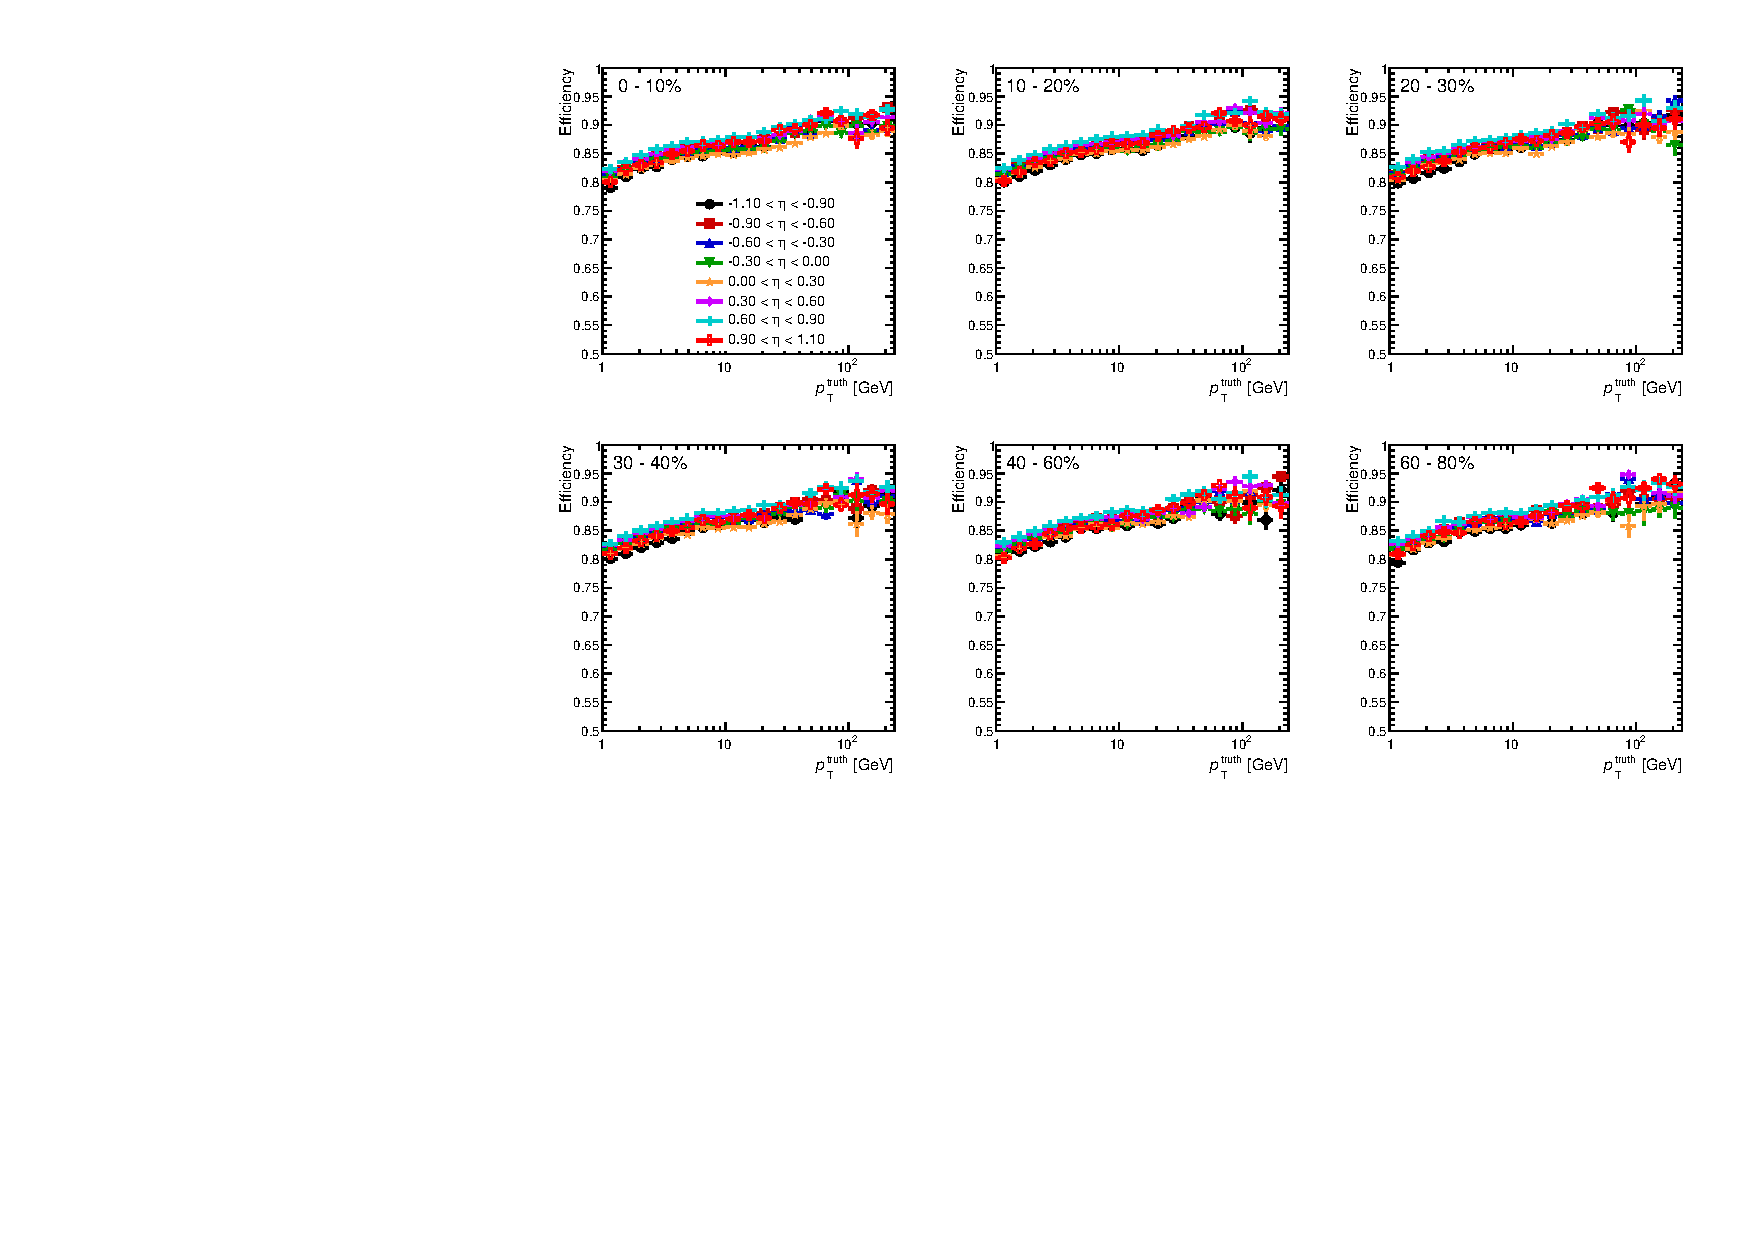
\includegraphics[width=0.9\textwidth]{figures_corrections/eff_cent_trketa_PbPb_ppTight.pdf}
   }
   \caption{Efficiency for reconstructing tracks evaluated using the default tracking selections in different track \eta\ bins in the data overlay \pbpb\ MC samples. Each panel is a different centrality bin..}
   \label{fig:pbpbeffdefault_final}
\end{figure}

\begin{figure}[ht]
   \centerline{
      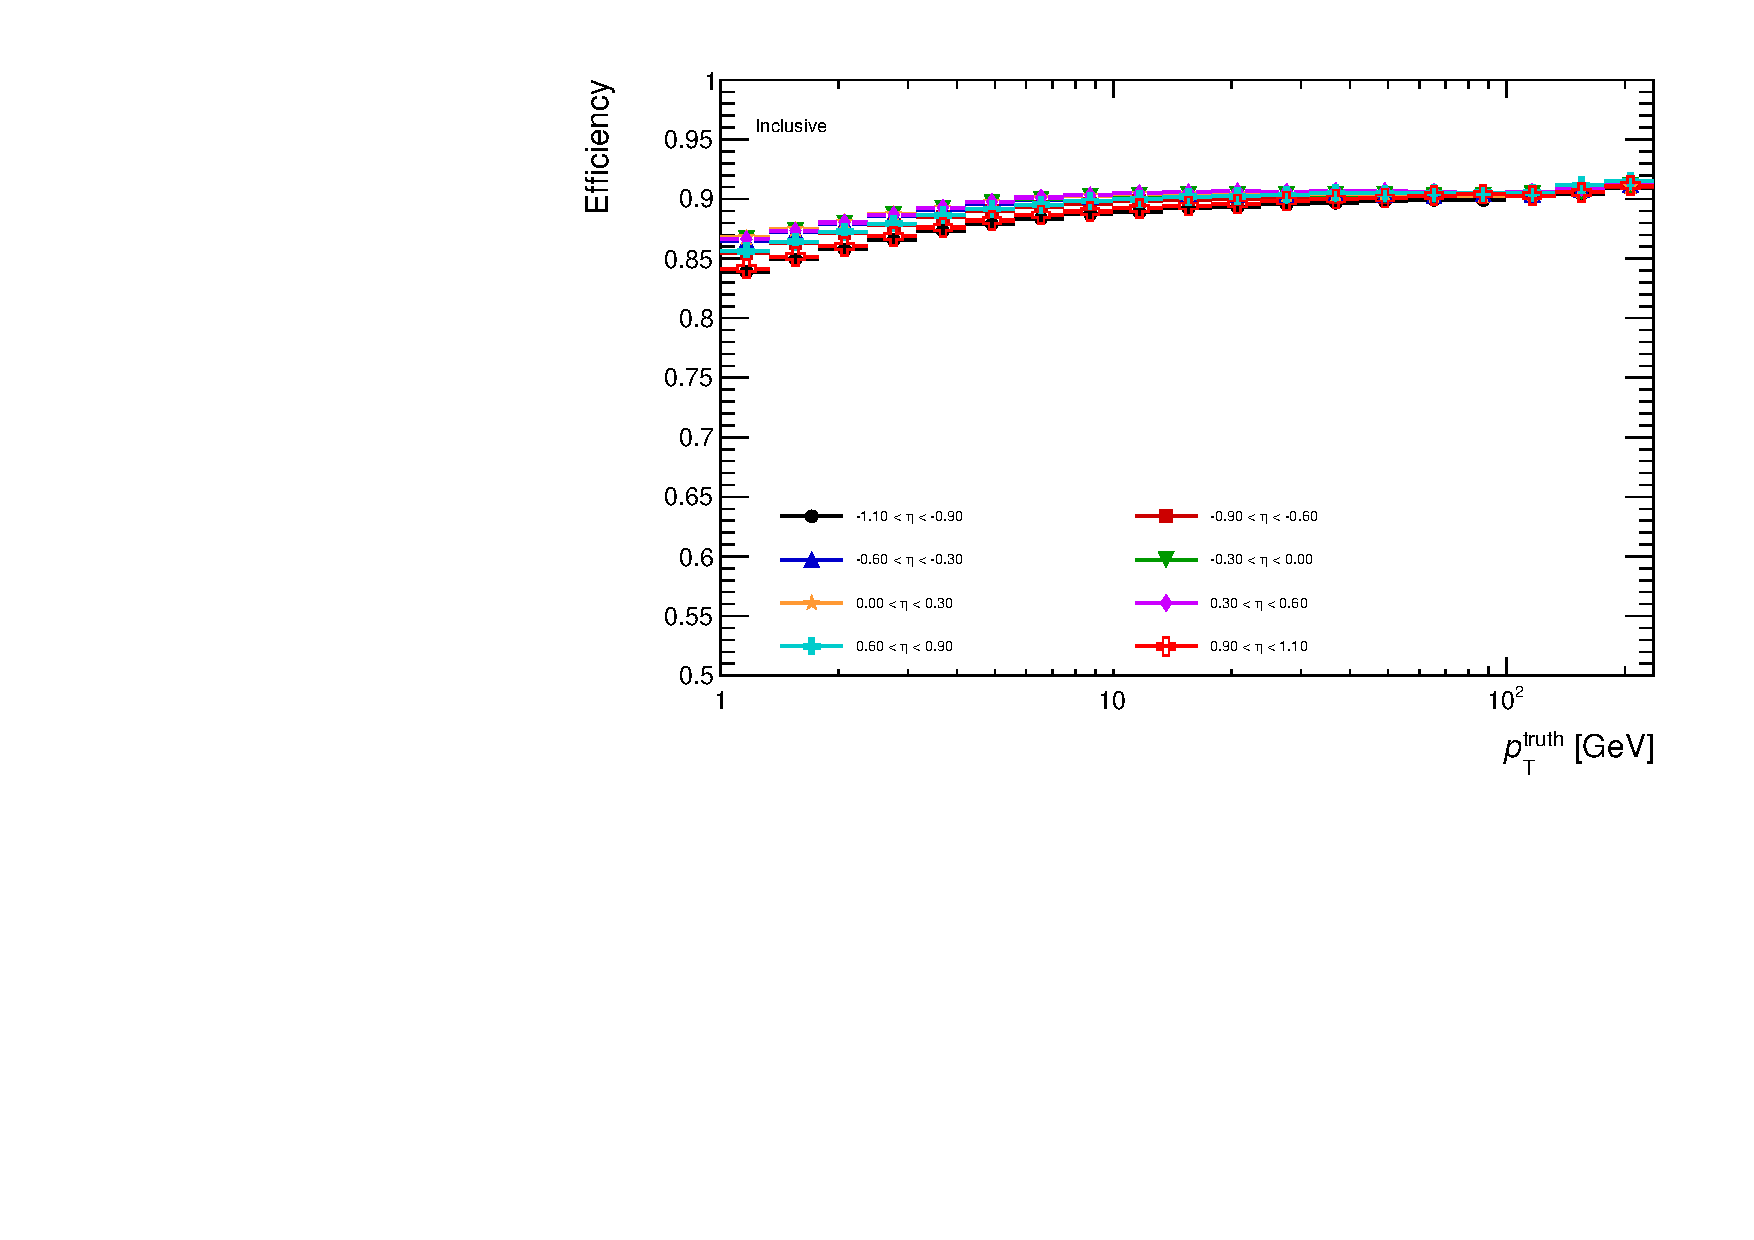
\includegraphics[width=0.55\textwidth]{figures_corrections/eff_cent_trketa_pp_ppTight.pdf}
   }
   \caption{Efficiency for reconstructing tracks evaluated using the default tracking selections in different track \eta\ bins in the \pp\ MC samples.}
   \label{fig:ppeffdefault_final}
\end{figure}

The final efficiency corrections applied were determined and applied as a function track \pt\ and track \eta, and can be seen in Figures~\ref{fig:pbpbeffdefault_final}-\ref{fig:ppeffdefault_final} for \pp\ and \PbPb\ collisions. No significant dependence on the collision centrality is observed. The efficiency exhibits a small, but monotonic increase with the track \pt. Only a small variation with the track $\eta$ is observed in the region $|\eta|<1.1$ The efficiency correction is applied on a track-by-track basis, assuming $\pttrk = \pTtrue$. While that assumption is not strictly valid, the efficiency varies sufficiently slowly with $\pTtrue$ that the error introduced by this assumption is negligible, up to 1\%. The tracking efficiency determined in Ref.~\cite{ATLAS502FFConf} was not seen to be dependent on \ptjet\ for $\pttrk \lesssim 40$ GeV as can be seen in Fig.~\ref{fig:pbpbeffdefaultjetpt_y0}-\ref{fig:ppeffdefaultjetpt}. The small depletion of the efficiency for tracks with $\pt \sim 10-40$~GeV was attributed to the convolution of how jet fragments and with the performance of the track reconstruction in the dense core of the jet~\cite{ATLAS502FFConf}. 


\begin{figure}[ht]
   \centerline{
      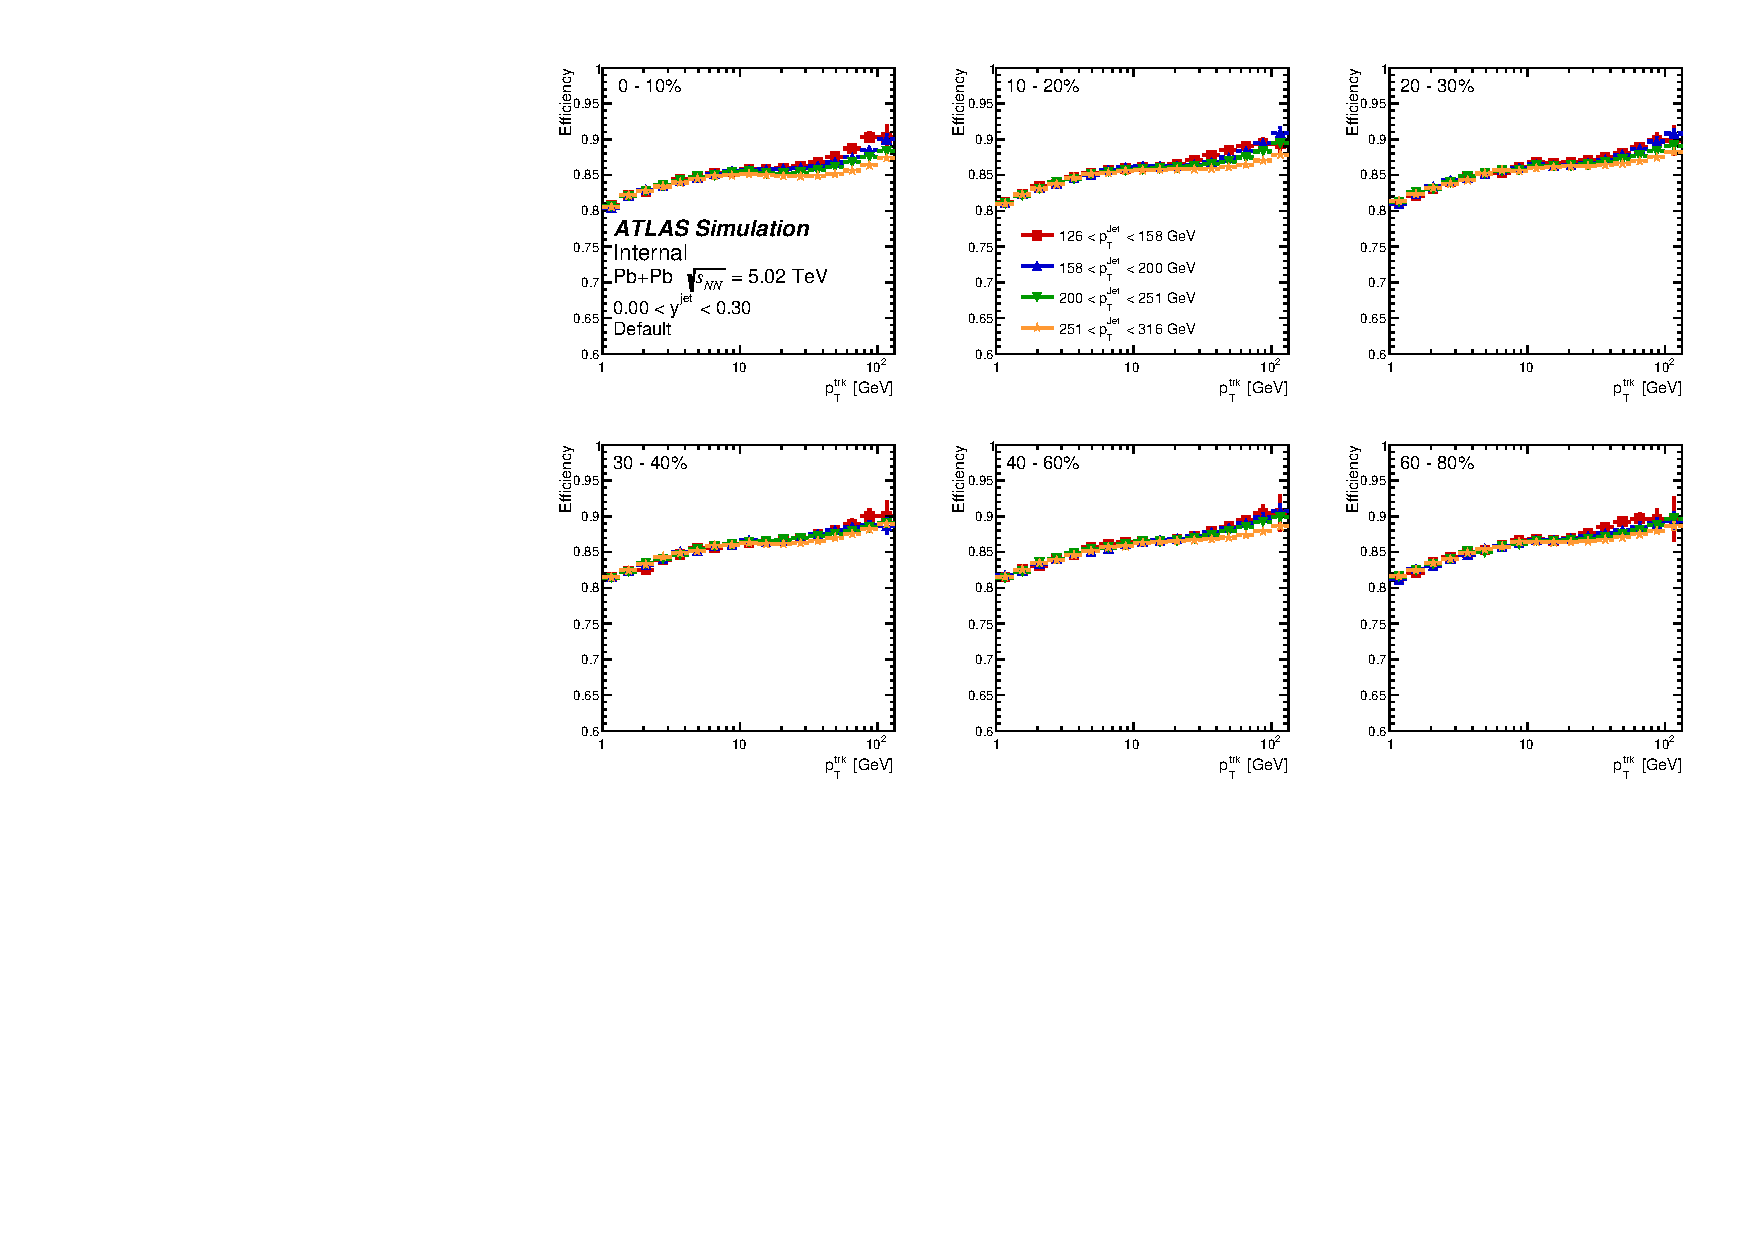
\includegraphics[width=0.9\textwidth]{figures_corrections/eff_centrality_jetpt_jety0_ppTight.pdf}
   }
   \caption{Efficiency for reconstructing tracks evaluated using the default tracking selections in different jet \pT\ bins and jet rapidity interval $|y|<0.3$ in the data overlay \pbpb\ MC samples. Each panel is a different centrality bin..}
   \label{fig:pbpbeffdefaultjetpt_y0}
\end{figure}

\begin{figure}[ht]
   \centerline{
      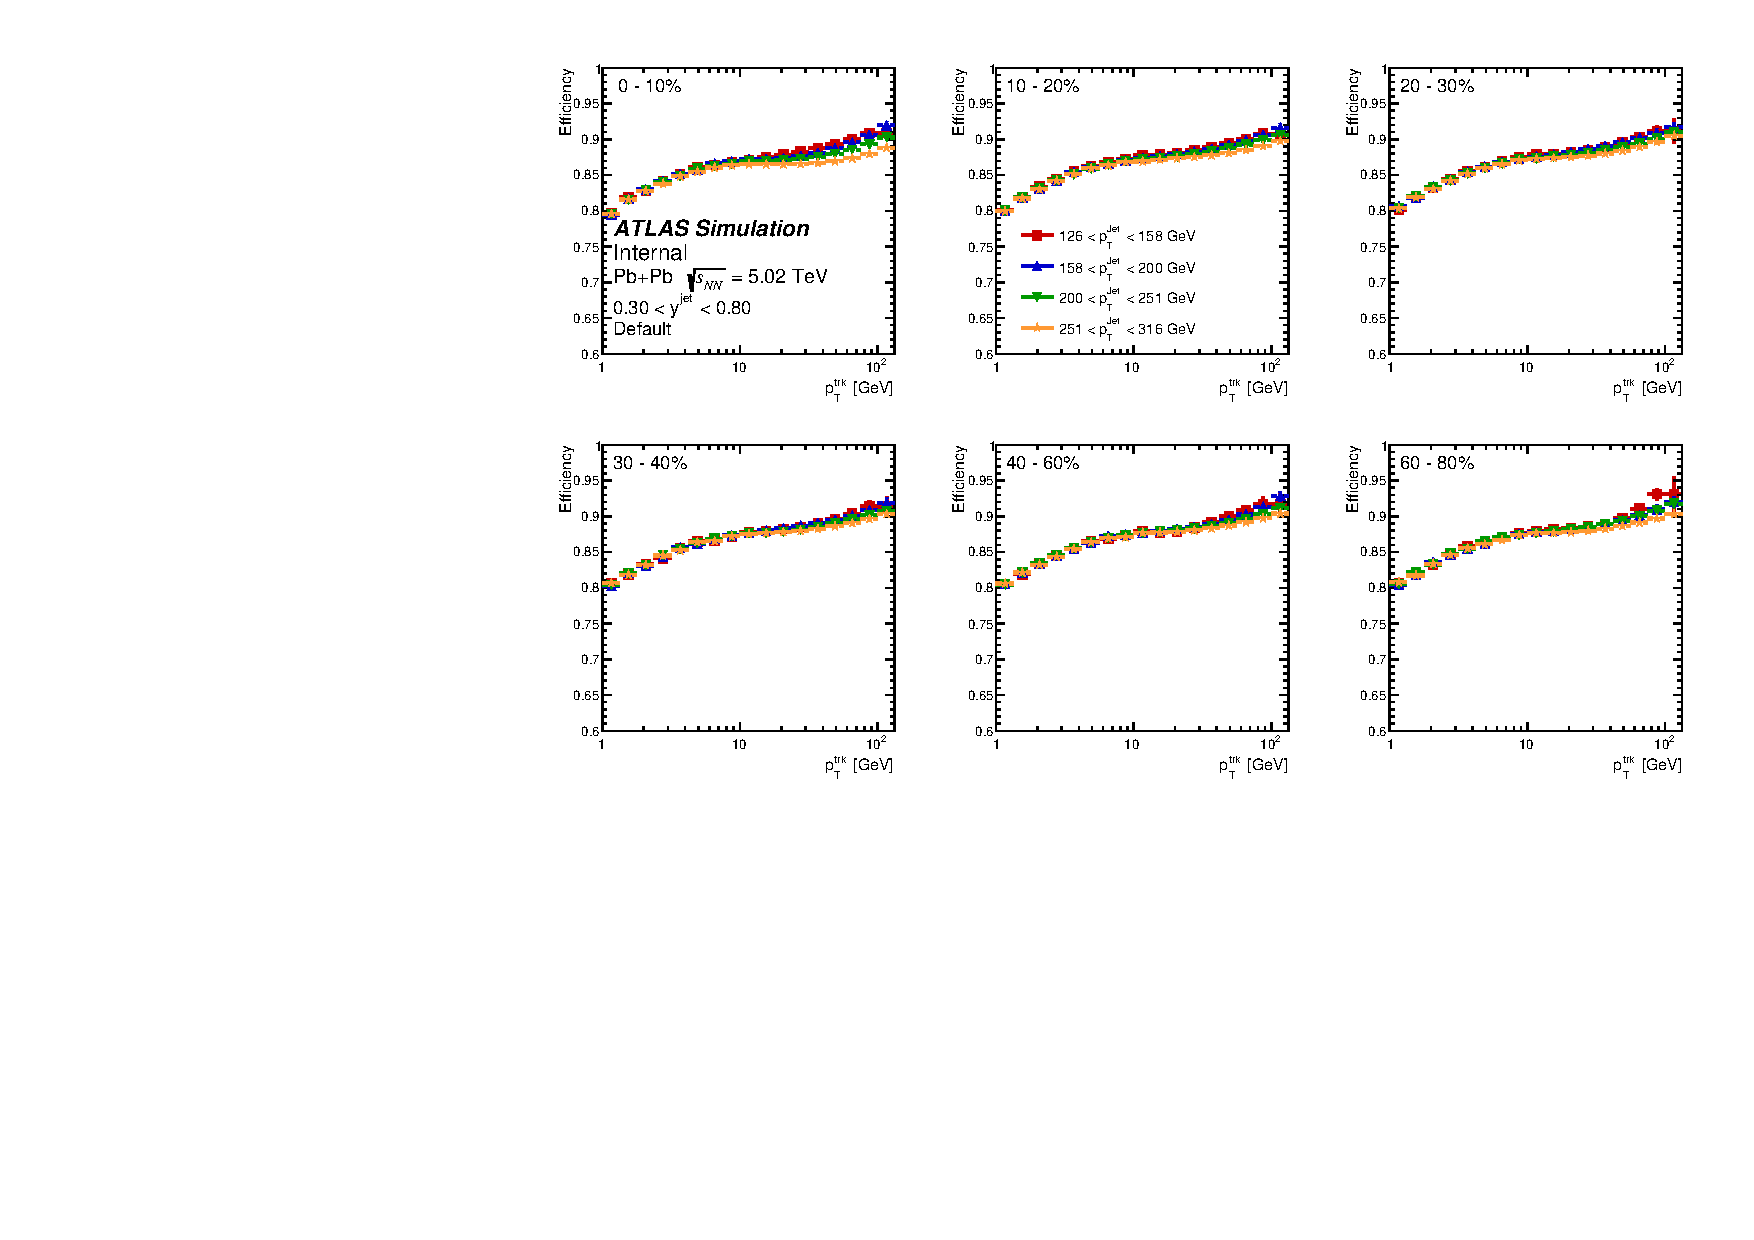
\includegraphics[width=0.9\textwidth]{figures_corrections/eff_centrality_jetpt_jety1_ppTight.pdf}
   }
   \caption{Efficiency for reconstructing tracks evaluated using the default tracking selections in different jet \pT\ bins and jet rapidity interval $0.3<|y|<0.8$ in the data overlay \pbpb\ MC samples. Each panel is a different centrality bin..}
   \label{fig:pbpbeffdefaultjetpt_y1}
\end{figure}

\begin{figure}[ht]
   \centerline{
      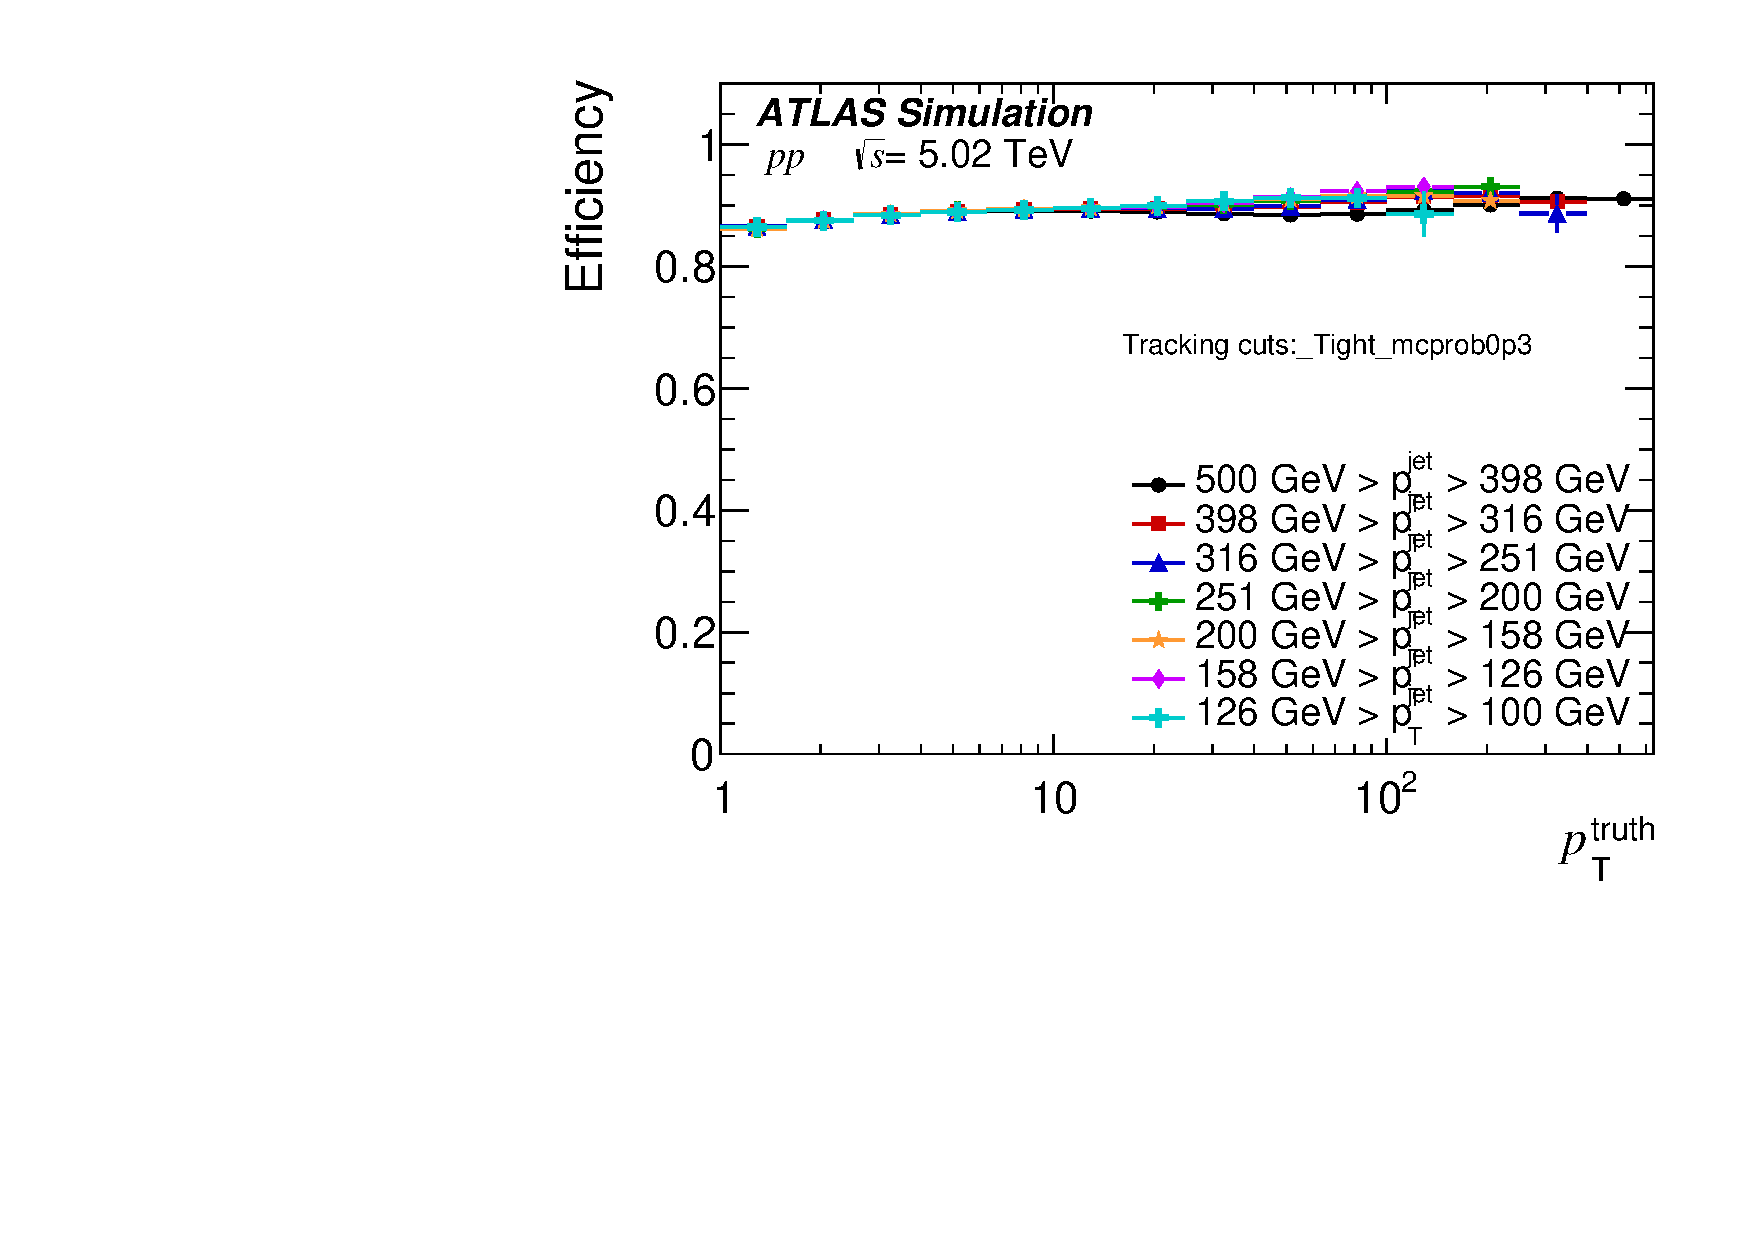
\includegraphics[width=0.55\textwidth]{figures_corrections/Trk_eff_v_pt_r005f_Tight_mcprob0p3_CX_Injet_0p0_0p3_pp_5p02.pdf}
   }
   \caption{Efficiency for reconstructing tracks evaluated using the default tracking selections in different jet \pT\ bins, in the \pp\ MC samples. }
   \label{fig:ppeffdefaultjetpt}
\end{figure}

\clearpage


\subsection{Fake rates}
\label{sec:fakerates}

The rate of fake tracks was evaluated and extensively studied in Ref.~\cite{ATLAS502FFConf} in the \pp, \pbpb\ HIJING MC, and in \pbpb\ MC+overlay samples. The MC overlay sample is used to crosscheck the fake rate at higher \pt, but is not used for any corrections. It was shown that as the \pttrk\ approaches the  \ptjet\ the fraction of fake tracks increases due to the steeply falling spectra of generator level tracks. Figures~\ref{fig:fakeratepp} and~\ref{fig:fakeratepbpb} show the fraction of tracks that are identified as fakes, secondaries, or part of UE in case of \PbPb\ collisions as a function of \pttrk\ for selections in \ptjet in
\pp\ and \pbpb\ collisions, respectively.  The rate 
decreases with \pttrk\ up to approximately 10~GeV and then remains constant until \pttrk\ approaches \ptjet\
where the rate increases again.  In \pbpb\ collisions, the ``fake'' rate also includes tracks which are from the underlying event from the real collisions into which the jet is overlaid.  The rate of these underlying event tracks increases with decreasing \pttrk\ and increasing collision centrality. The contribution from UE is negligible for tracks with \pT\ above 10 GeV as no centrality dependence is seen. The Fig.~\ref{fig:fakeratepbpb} excludes the very low \pT\ region where the distribution would be completely dominated by the UE. The size of the UE is then presented further in Fig.~\ref{fig:UEimpact_r2}-\ref{fig:UEimpact_r6}. To separate the contribution of UE tracks (see section~\ref{sec:cuts_UE}) from the fake tracks in \PbPb\ collisions and cross-check the centrality dependence of the fake rate, 0.2M MB \PbPb\ fully reconstructed HIJING MC~\cite{Wang:1991hta} events was used. The HIJING MC generator is capable of simulating global properties of HI collisions. The estimated fake rate of tracks associated with jets with $\pT>40 GeV$ is at the level of 1\% and it exhibits similar behavior as observed in Fig.~\ref{fig:fakeratepbpb}. No significant dependence of the fake rate on the collision centrality was found~\cite{ATLAS502FFConf}.
  
  \begin{figure}[ht]
  \centerline{
  \begin{tabular}{cc}
  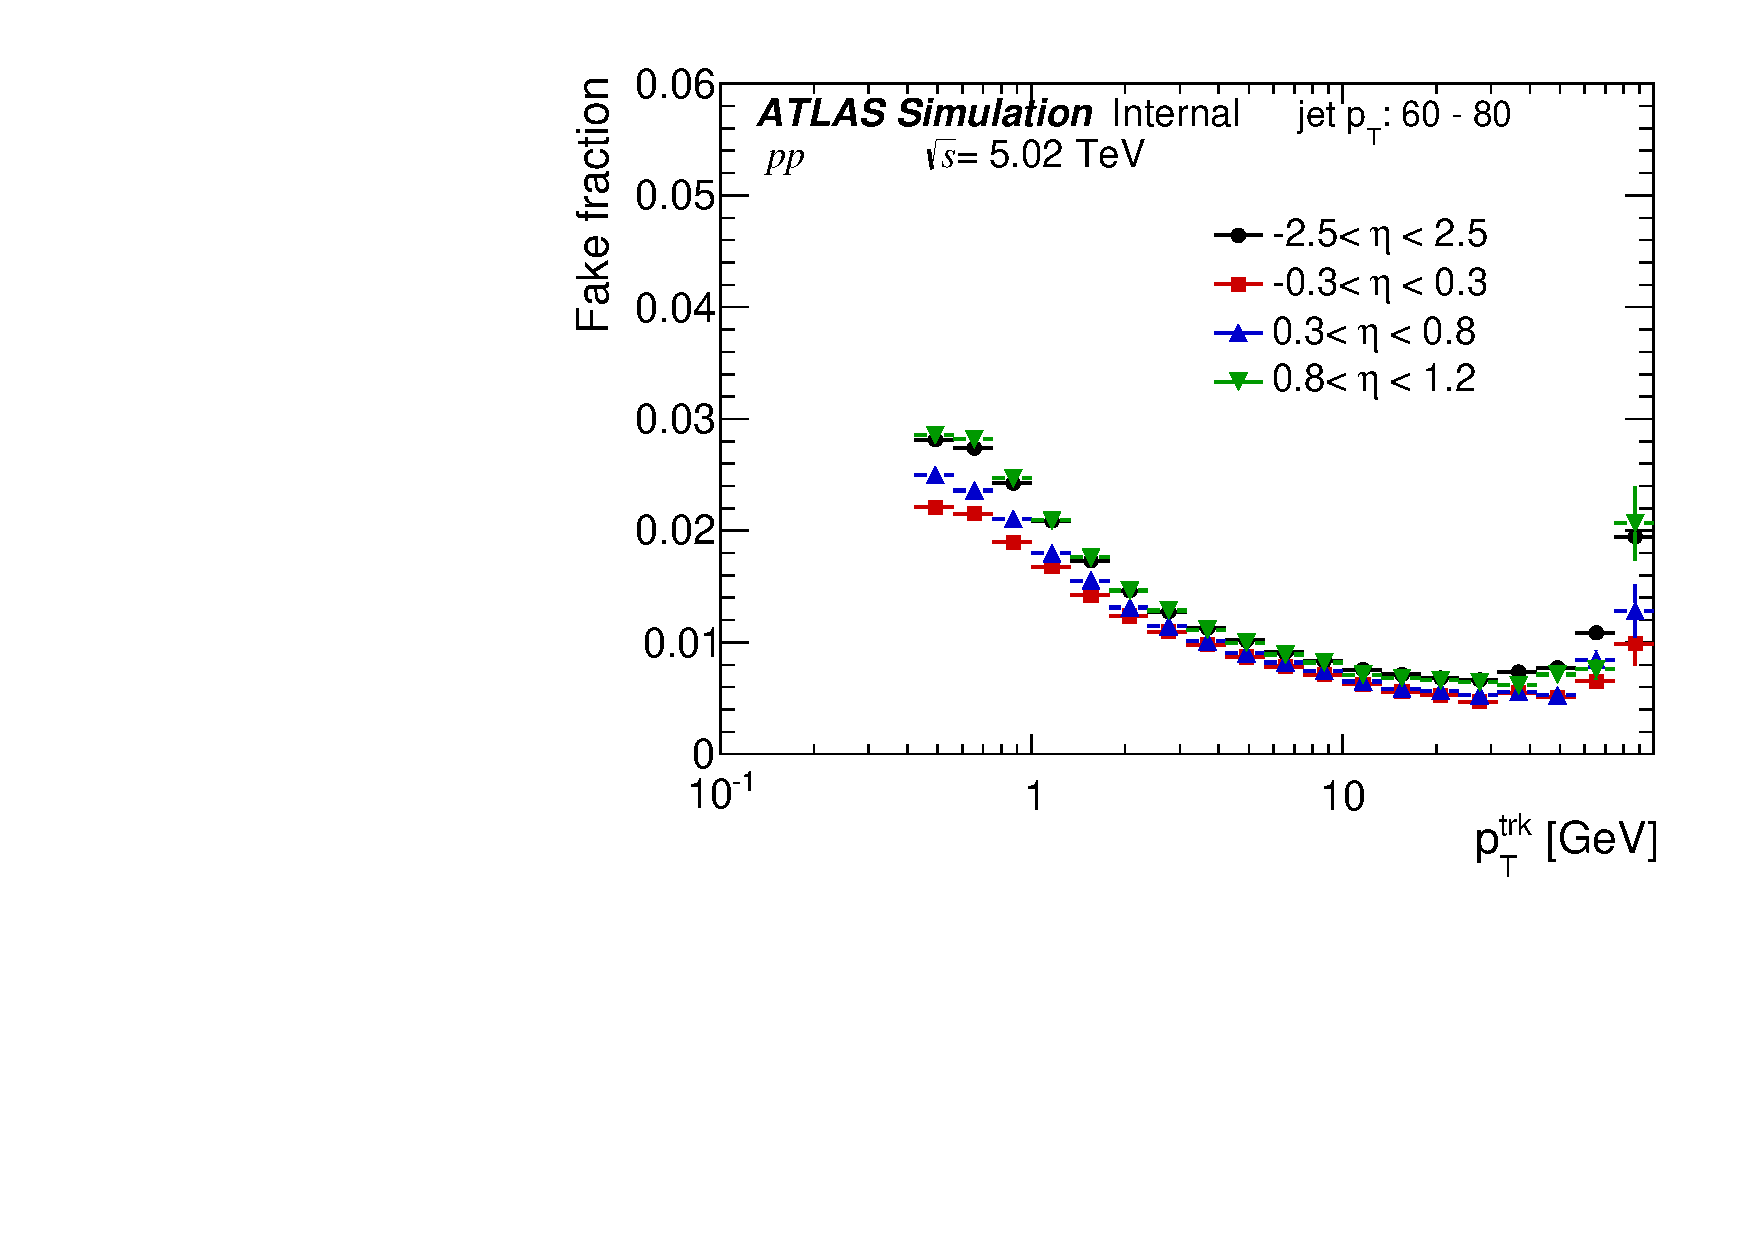
\includegraphics[width=0.45\textwidth]{figures_corrections/fake_rates/FakesEta_pp_5p02_r003_Tight_mcprob0p3_JZ2_jetpt_2.pdf} &
  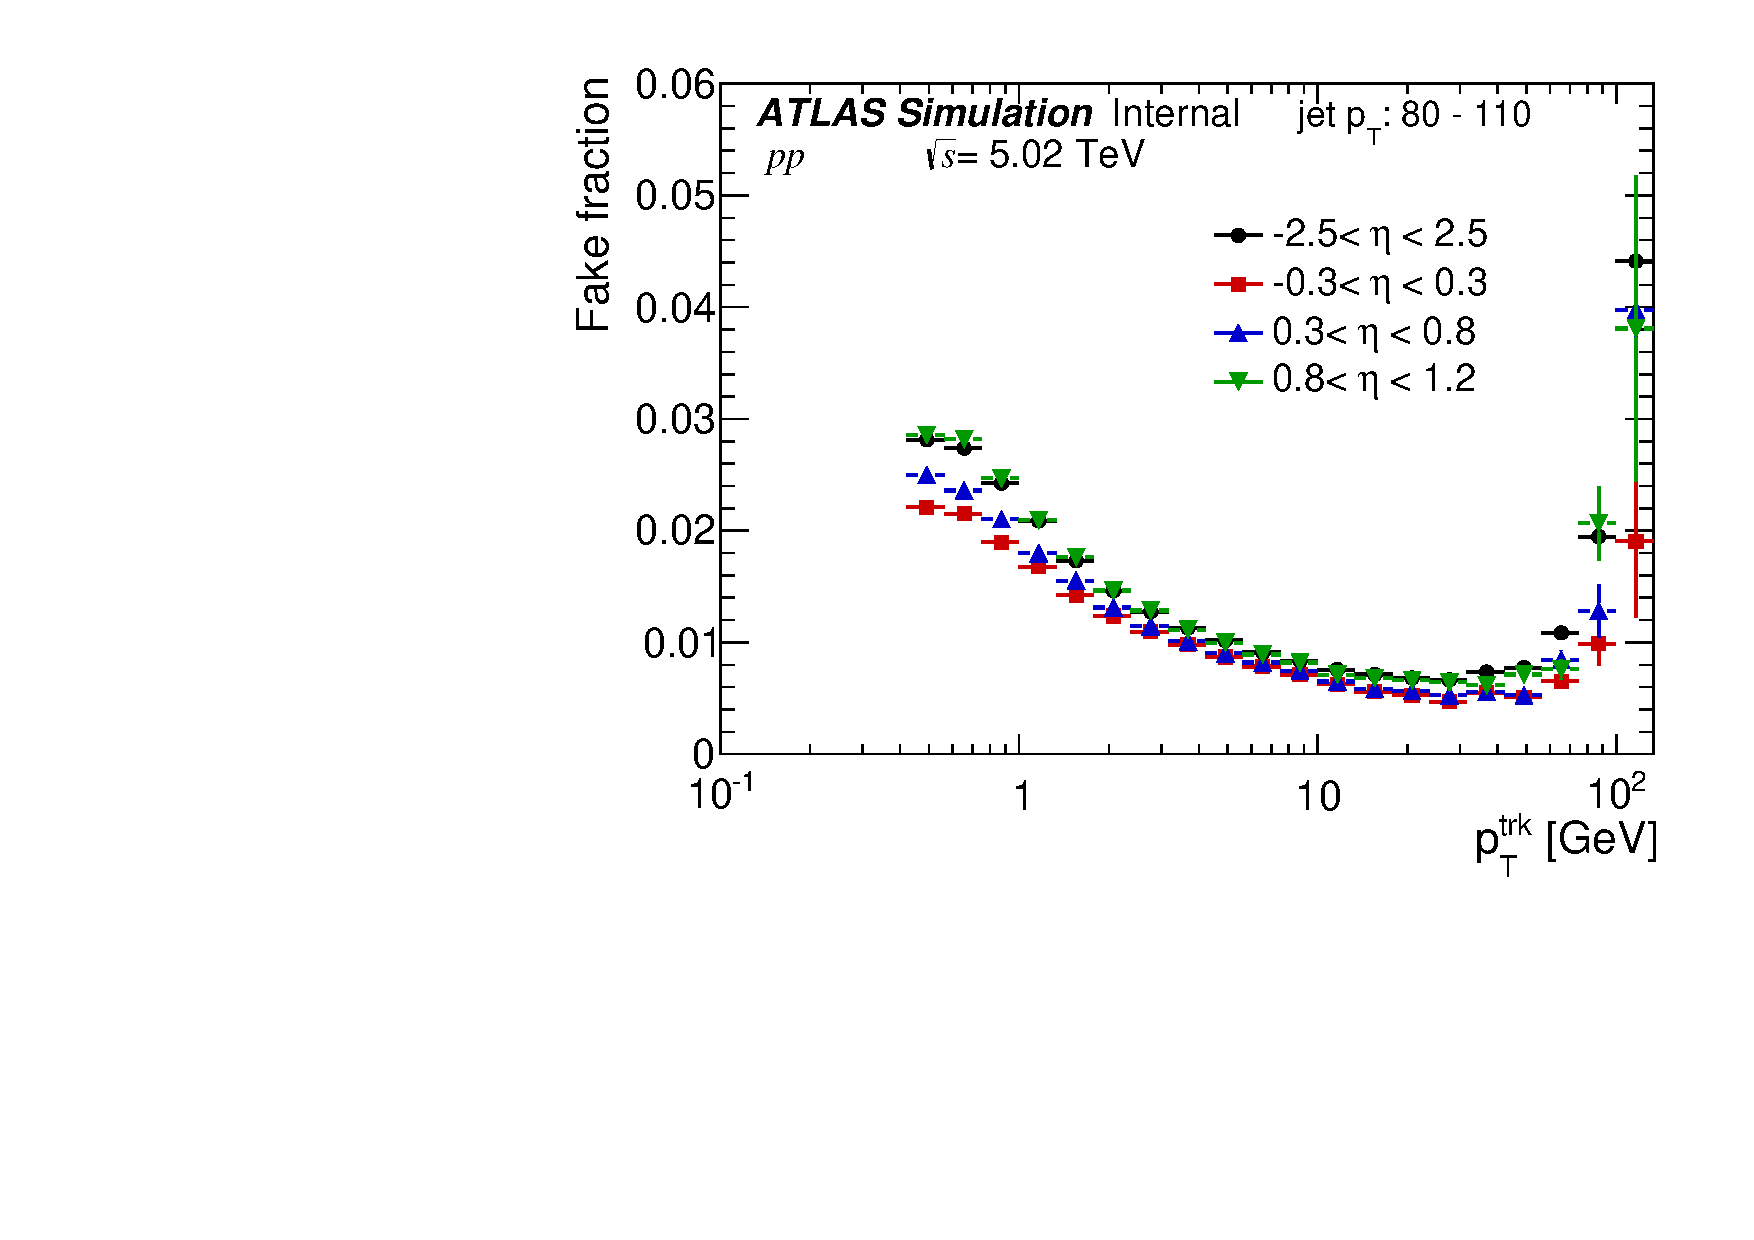
\includegraphics[width=0.45\textwidth]{figures_corrections/fake_rates/FakesEta_pp_5p02_r003_Tight_mcprob0p3_JZ2_jetpt_3.pdf} \\
    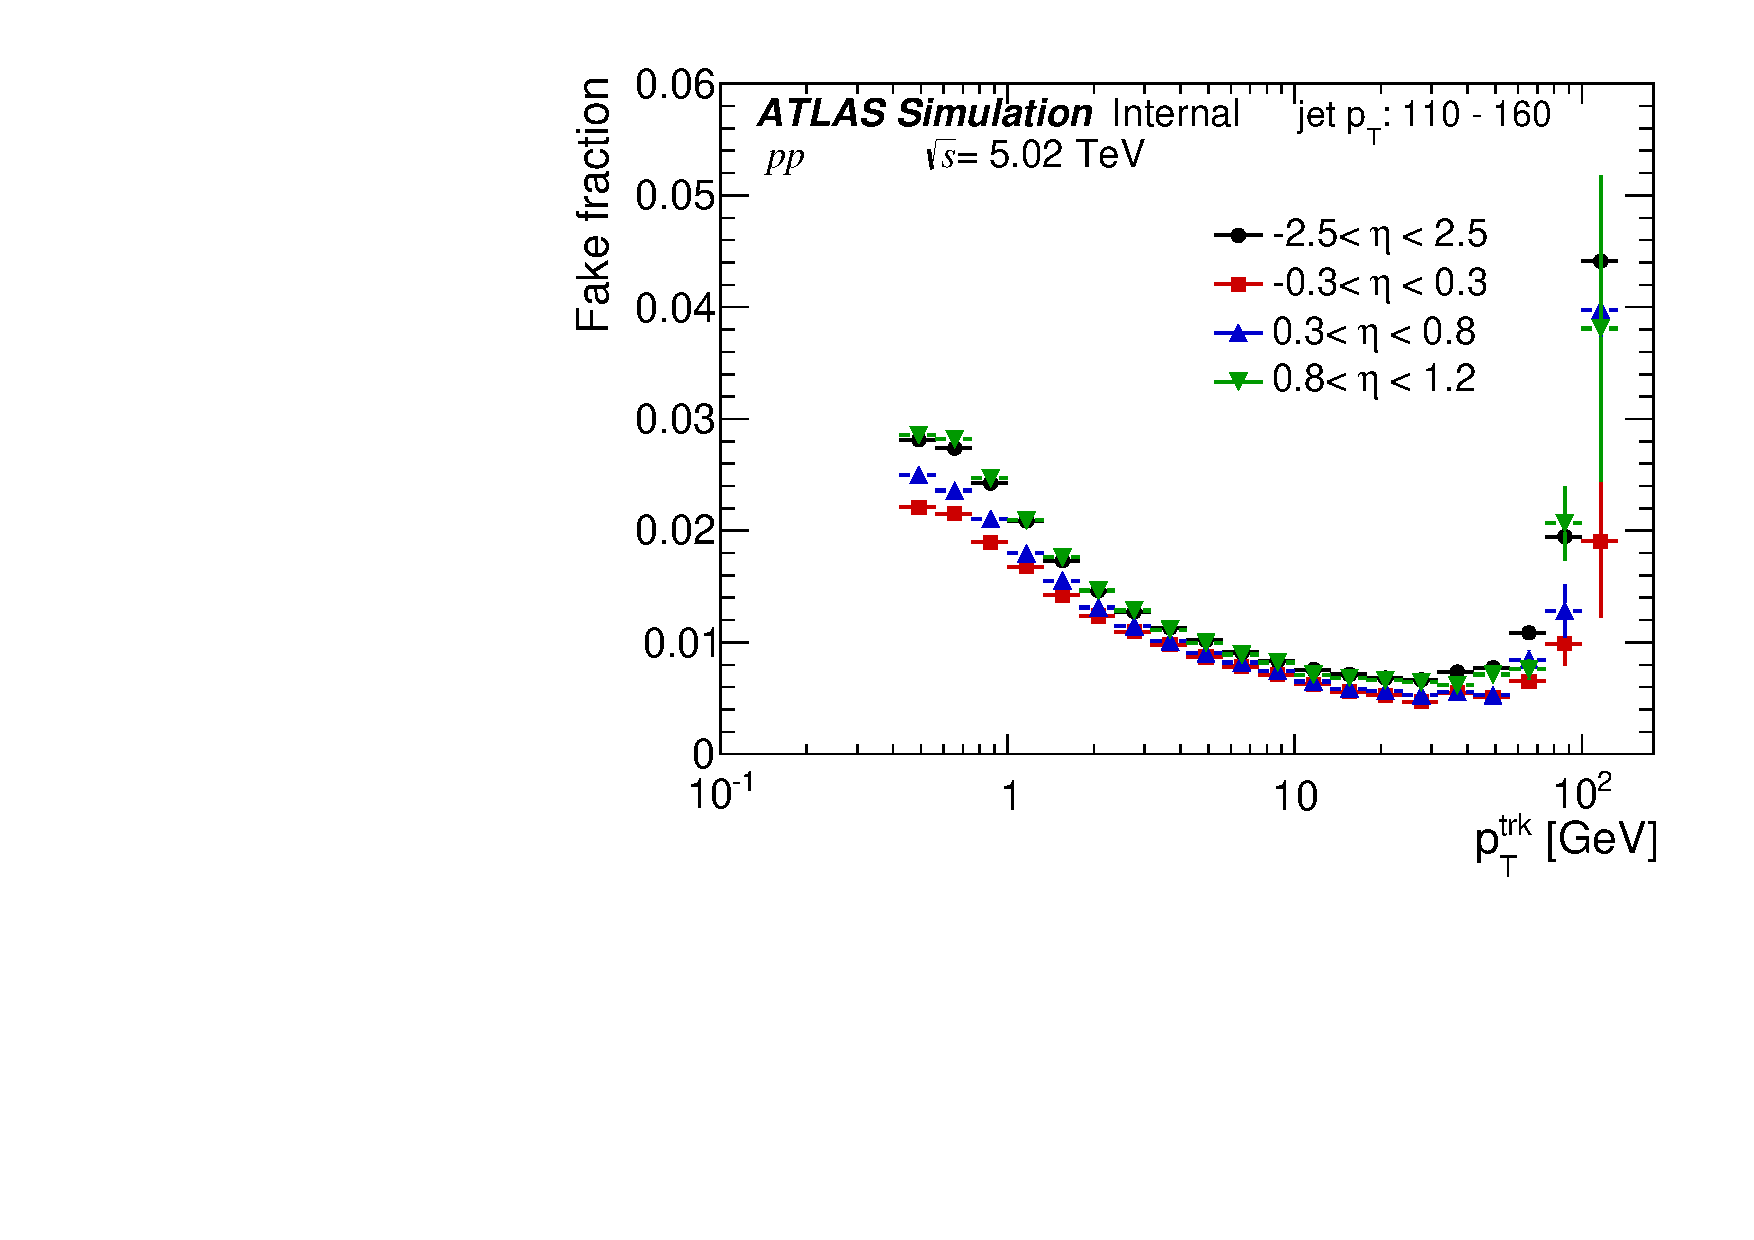
\includegraphics[width=0.45\textwidth]{figures_corrections/fake_rates/FakesEta_pp_5p02_r003_Tight_mcprob0p3_JZ2_jetpt_4.pdf} &
    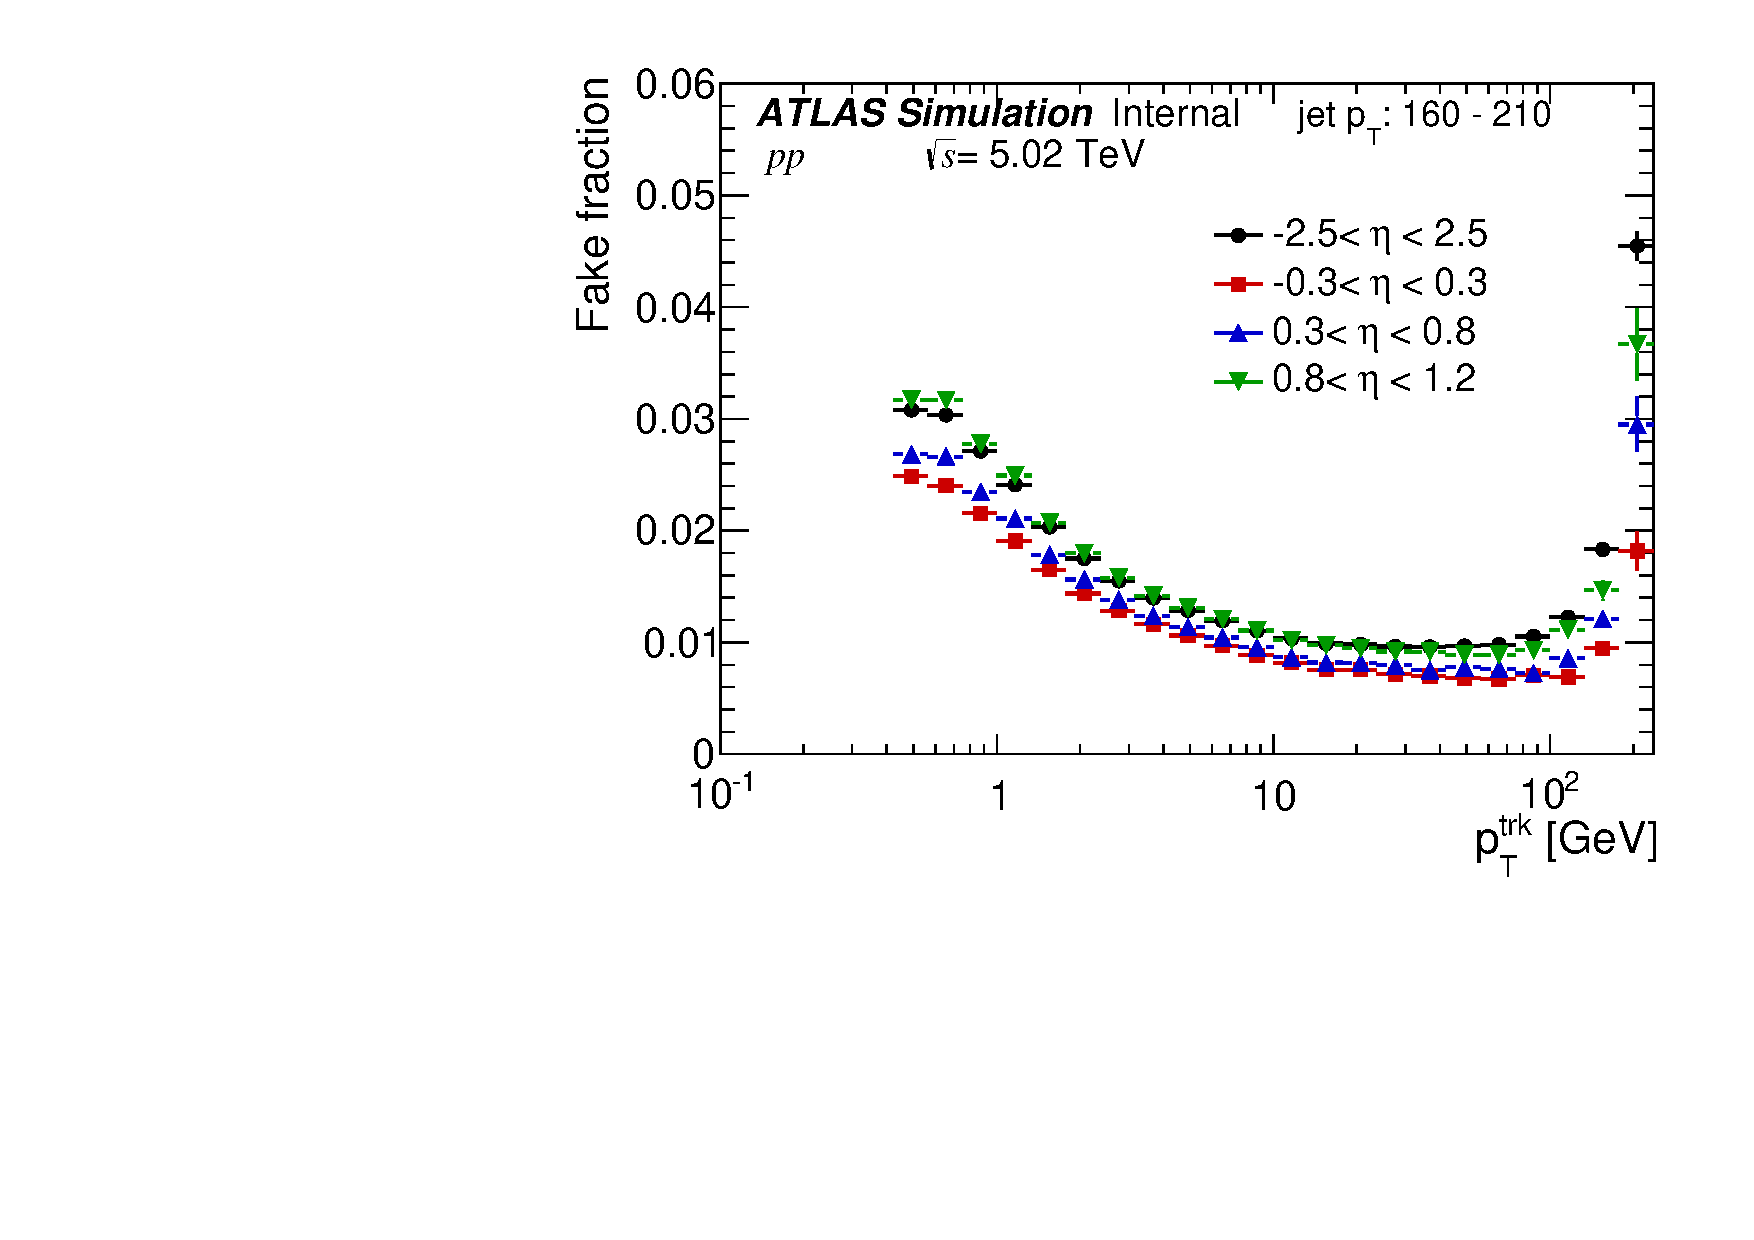
\includegraphics[width=0.45\textwidth]{figures_corrections/fake_rates/FakesEta_pp_5p02_r003_Tight_mcprob0p3_JZ3_jetpt_5.pdf} \\
      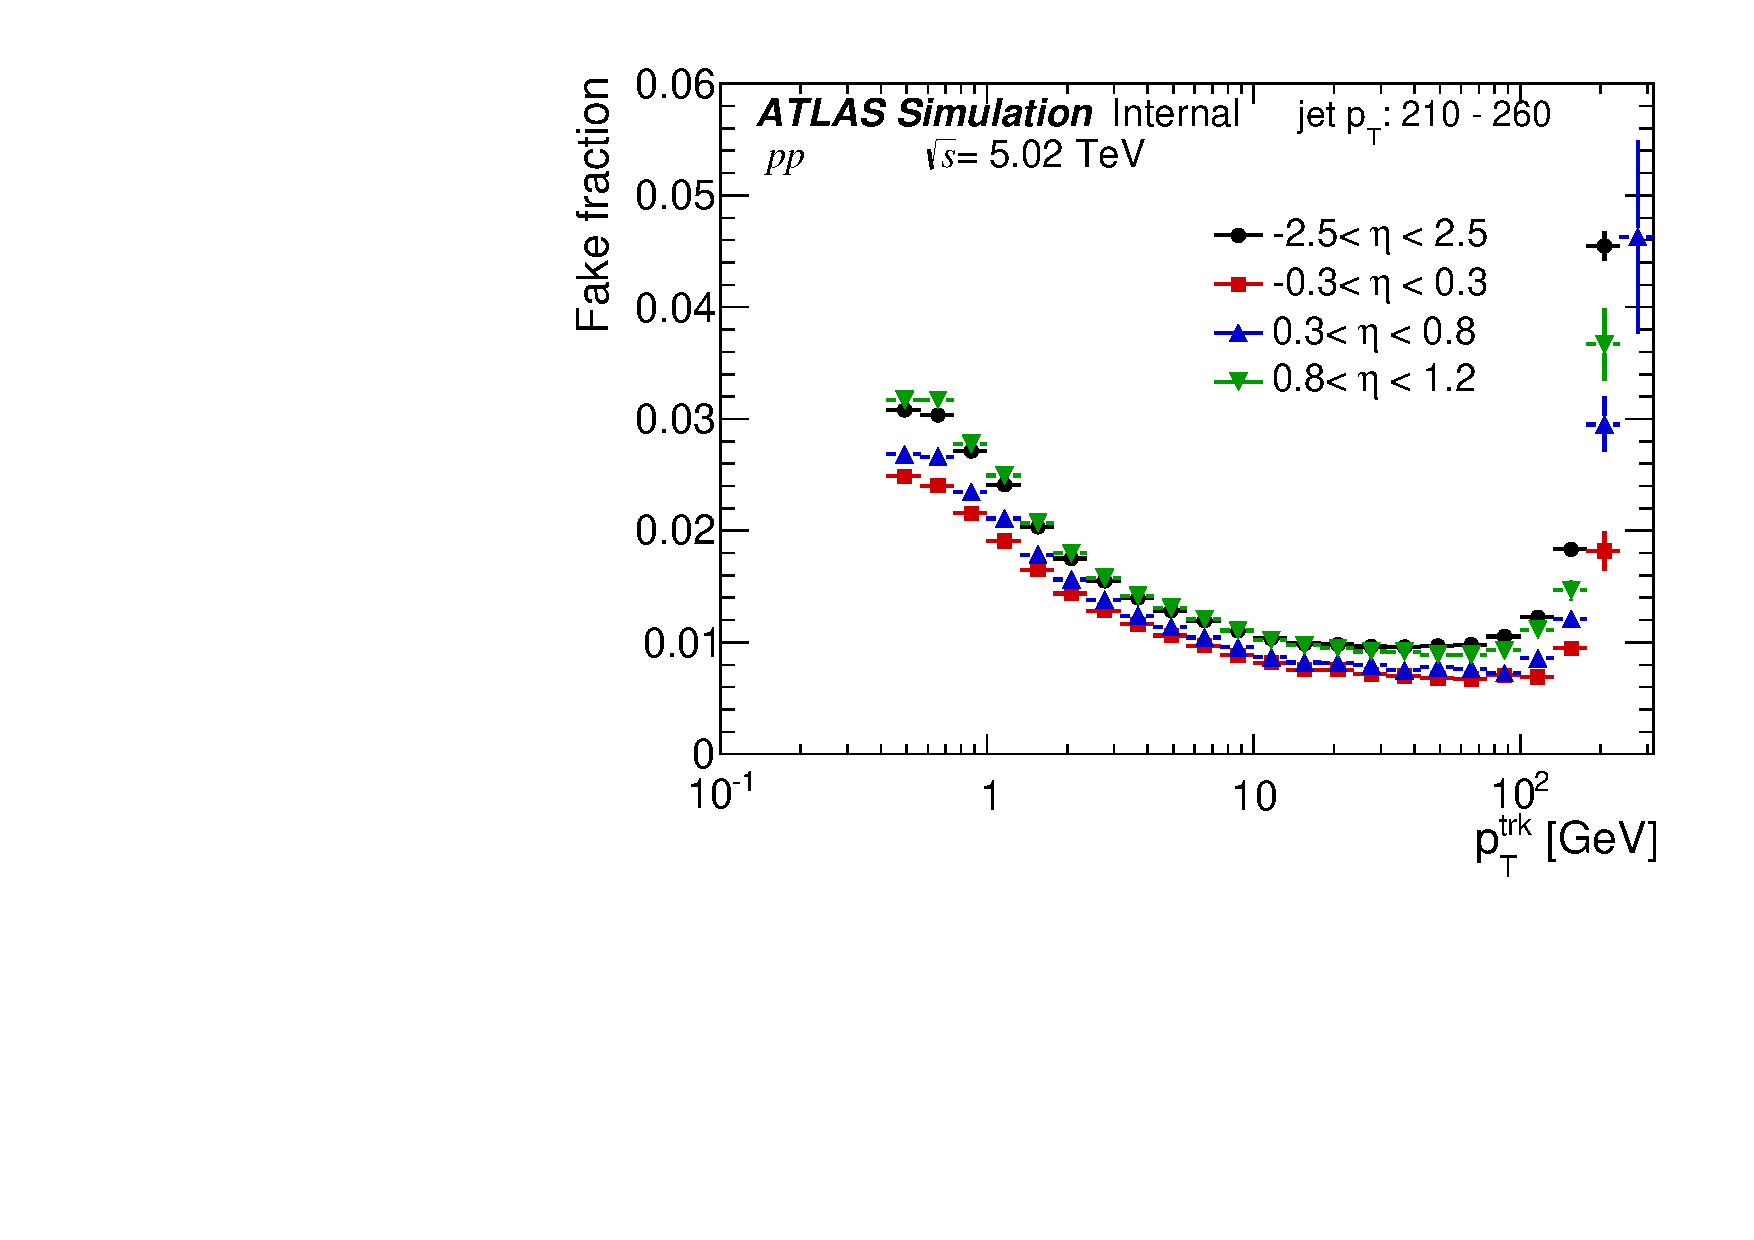
\includegraphics[width=0.45\textwidth]{figures_corrections/fake_rates/FakesEta_pp_5p02_r003_Tight_mcprob0p3_JZ3_jetpt_6.pdf} &
  \end{tabular}}
  \caption{Fake rate for five different \ptjet\ selections in 5.02 TeV \pp\ collisions and four pseudorapidity intervals. The fake rate is evaluated for default value of $MC_{\mathrm{prob}}$ cut of 0.3 used in 2015 analysis.}
  \label{fig:fakeratepp}
  \end{figure}  

  \begin{figure}[ht]
     \centerline{
	\begin{tabular}{cc}
	   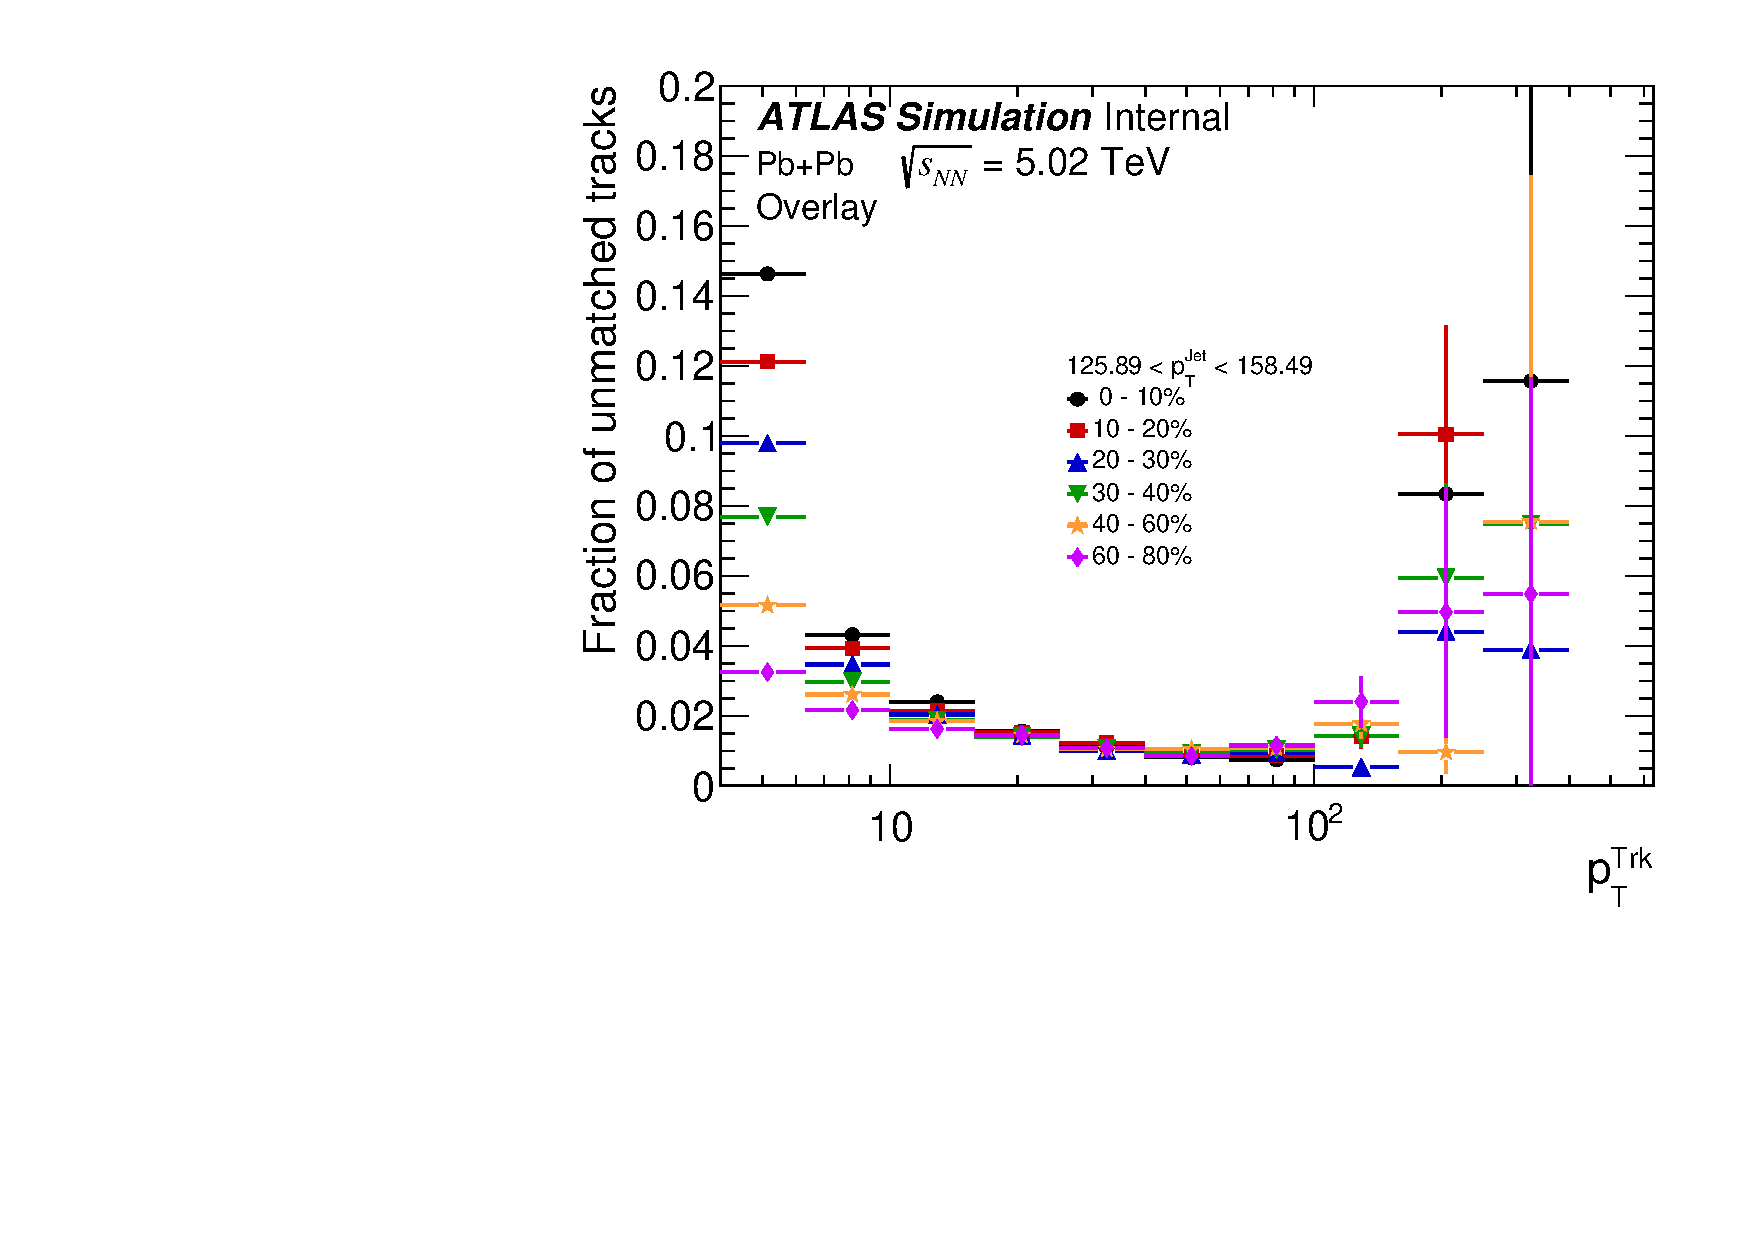
\includegraphics[width=0.45\textwidth]{figures_corrections/fake_rate_pt_125GeV.pdf} &
	   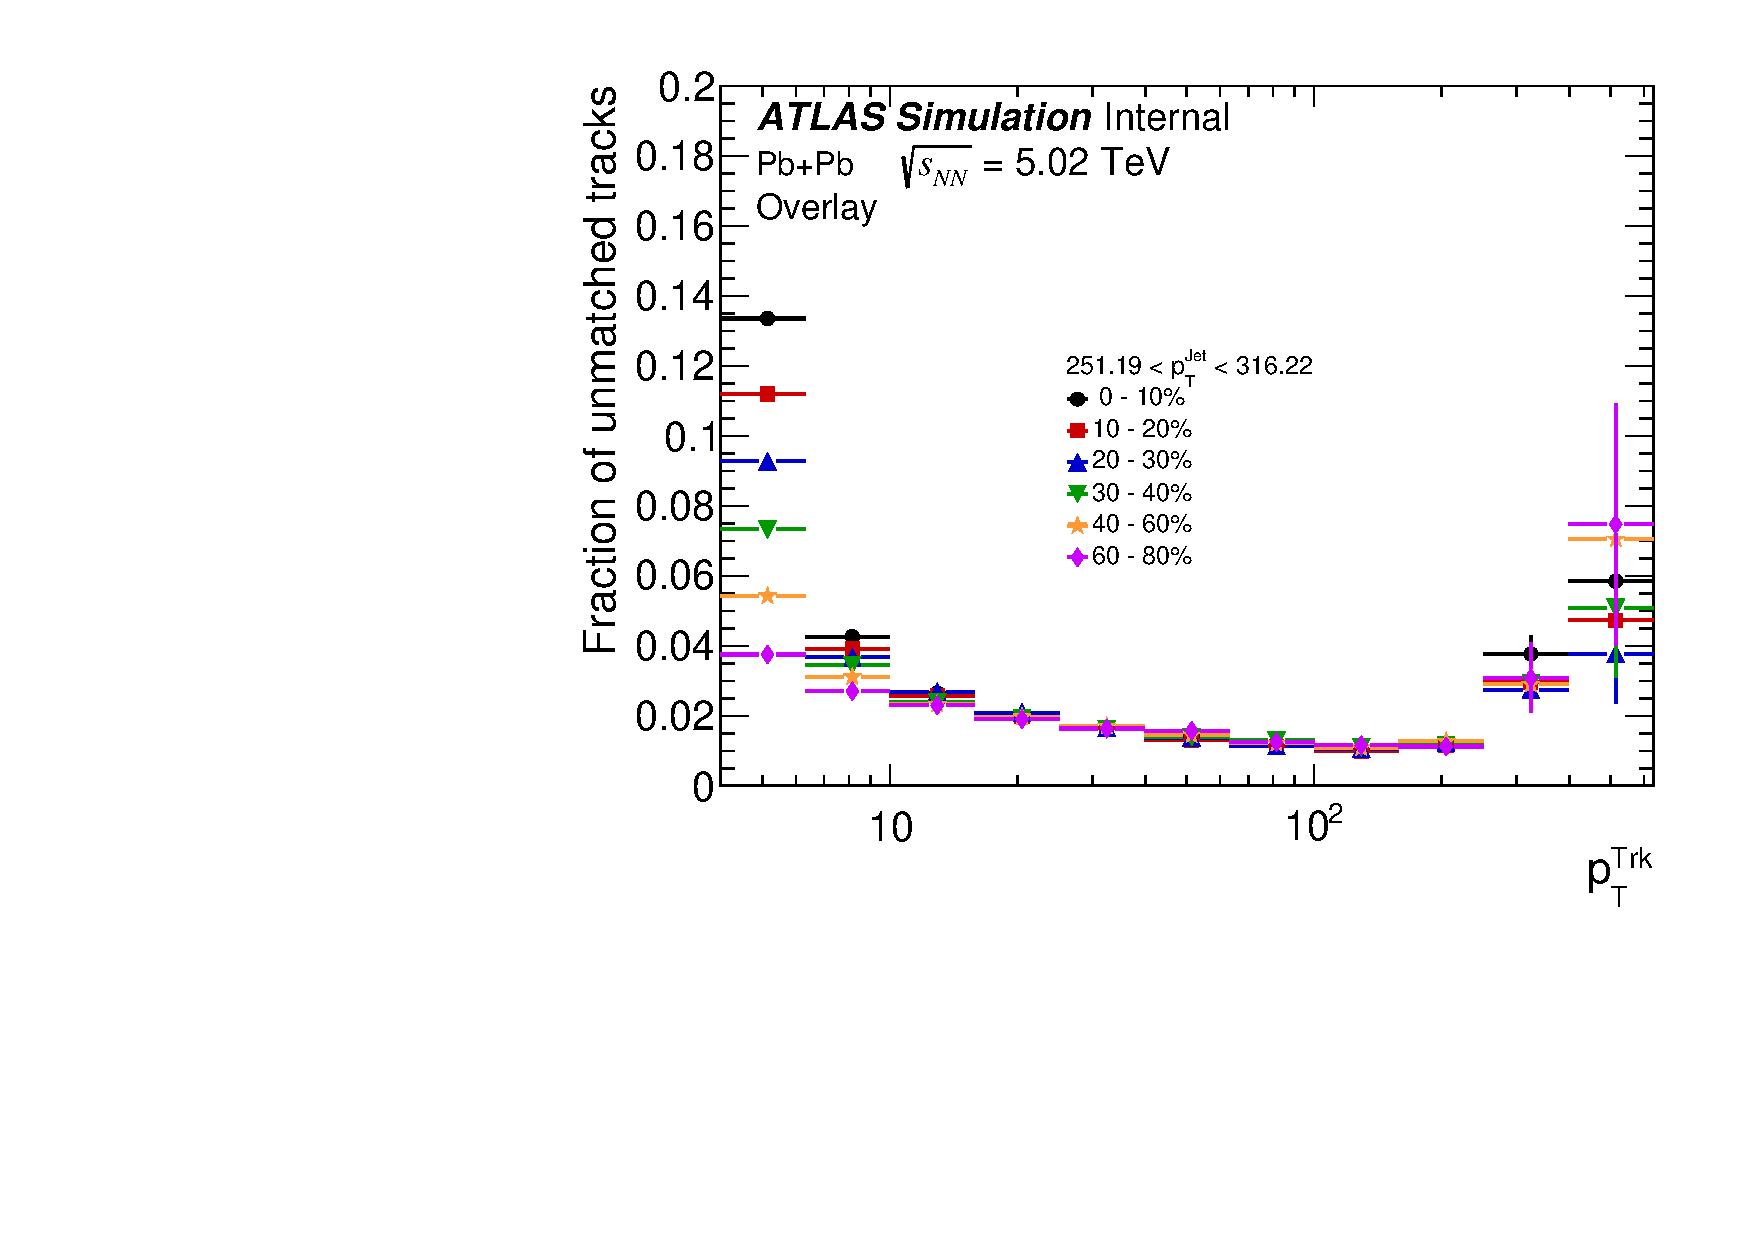
\includegraphics[width=0.45\textwidth]{figures_corrections/fake_rate_pt_251GeV.pdf} \\
	\end{tabular}
     }
     \caption{ Rate of tracks unmatched to truth tracks
	in \pbpb\ collisions for different centrality selections as indicated on the plot as a function of \pttrk.  
	The unmatched tracks include both fake tracks and tracks from the underlying event.  The panels show
	two \ptjet\ selections: 126-158~GeV (left) and 251-316~GeV (right). The low \pT\ part is omitted as it is dominated by the contribution from the UE.}
     \label{fig:fakeratepbpb}
  \end{figure}


To correct for the contribution from fake and secondary particles, $\Dptr^{TM}$ distributions are estimated in the similar way as measured \Dptr distributions, but only reconstructed tracks that do not not matched to truth tracks by criteria described in previous paragraphs are used. These fake $\Dptr^{TM}$ distributions are then subtracted from the measured distributions both in the data and MC. This procedure is applied for tracks above 10 GeV in \PbPb\ collisions and for tracks above 1 GeV in \pp\ collisions.  The correction also removes any residual UE above 10~GeV in case of \PbPb. The choice of the 10 GeV cut is based on the centrality dependence of the rate of truth-unmatched tracks in MC overlay samples shown in Fig.~\ref{fig:fakeratepbpb}. The correction for UE, fake and secondary tracks bellow 10 GeV in \PbPb\ collisions is discussed in the next section.

\clearpage

\subsection{Underlying event subtraction of tracks}
\label{sec:cuts_UE}

The underlying event subtraction performed on the calorimetric jet energy is described in Sec.~\ref{sec:reconstruction}. Charged particles from the nucleon-nucleon scatterings that are not associated with the hard scattering in question constitute a background to the \Dptr\ distributions that needs to be subtracted from the measured distributions. This background strongly depends on the collisions centrality and on the charged particle \pt. In the measurement of the inclusive jet fragmentation functions it was found that the UE contribution is negligible for charged particles with $\pt>10$~GeV~\cite{PbPb5TeVIntNote}. This can be seen in the centrality dependence of the combined rate of fake and underlying event charged particles shown in Fig.~\ref{fig:fakeratepbpb} where no significant centrality dependence is observed for track above 10 GeV. 


The UE contribution to a given annulus around the jet is estimated using MB events where the $\mathrm{d}N_{\mathrm{ch}}/\mathrm{d}\phi\mathrm{d}\eta(\mathrm{cent},\pt, \mathrm{d}\Psi_{\mathrm{ch}})$ distributions of charged particles are estimated, where $\Psi$ is determined from the energy of the forward calorimeter. These distribution are evaluated as a function of charged particle \pt, collision centrality and angular distance, $\mathrm{d}\Psi_{\mathrm{ch}}$, with respect to the reaction plane angle $\Psi$. They are then used to estimate average number of UE charged particles in given annulus around a jet, $\nchUE^{\mathrm{MB}}(\eta_{\mathrm{jet}}, \phi_{\mathrm{jet}}, \mathrm{d}\Psi_{\mathrm{jet}})$, with given $\eta_{\mathrm{jet}}$, $\phi_{\mathrm{jet}}$, and $\mathrm{d}\Psi_{\mathrm{jet}}$ positions. Examples of the $\nchUE^{\mathrm{MB}}$ distributions for three different annuli, three intervals of the angular distance between jet and the reaction plane,  two different collision centrality classes and charged particle \pt\ intervals are shown in Fig.~\ref{fig:nchcore1}-\ref{fig:nchcore3}. The number of UE particles associated with jet decreases with size of the annulus, decreasing centrality, increasing track \pT\ and increasing distance to the reaction plane. The difference in the centrality distribution between MB data and the jet triggered sample is accounted for by a reweighing procedure to match the centrality distribution in the jet triggered data samples.

The resulting UE charged particle contributions to measured \Dptr\ distributions, $\fd \nchUE/ \fd \pTch$ were evaluated over $1 < \pTch < 10$~\GeV\ as a function of charged particle \pT, \pTjet, and  collision centrality using the $\nchUE^{\mathrm{MB}}$ distributions convoluted with the $\eta_{\mathrm{jet}}$, $\phi_{\mathrm{jet}}$, and $\mathrm{d}\Psi_{\mathrm{jet}}$ distributions of jets in the jet triggered sample. By evaluating the UE yields only from events containing jets included in the analysis, the background automatically had the correct distribution of centralities within a given centrality bin.  

\begin{figure}[ht]
\centerline{
\begin{tabular}{ccc}
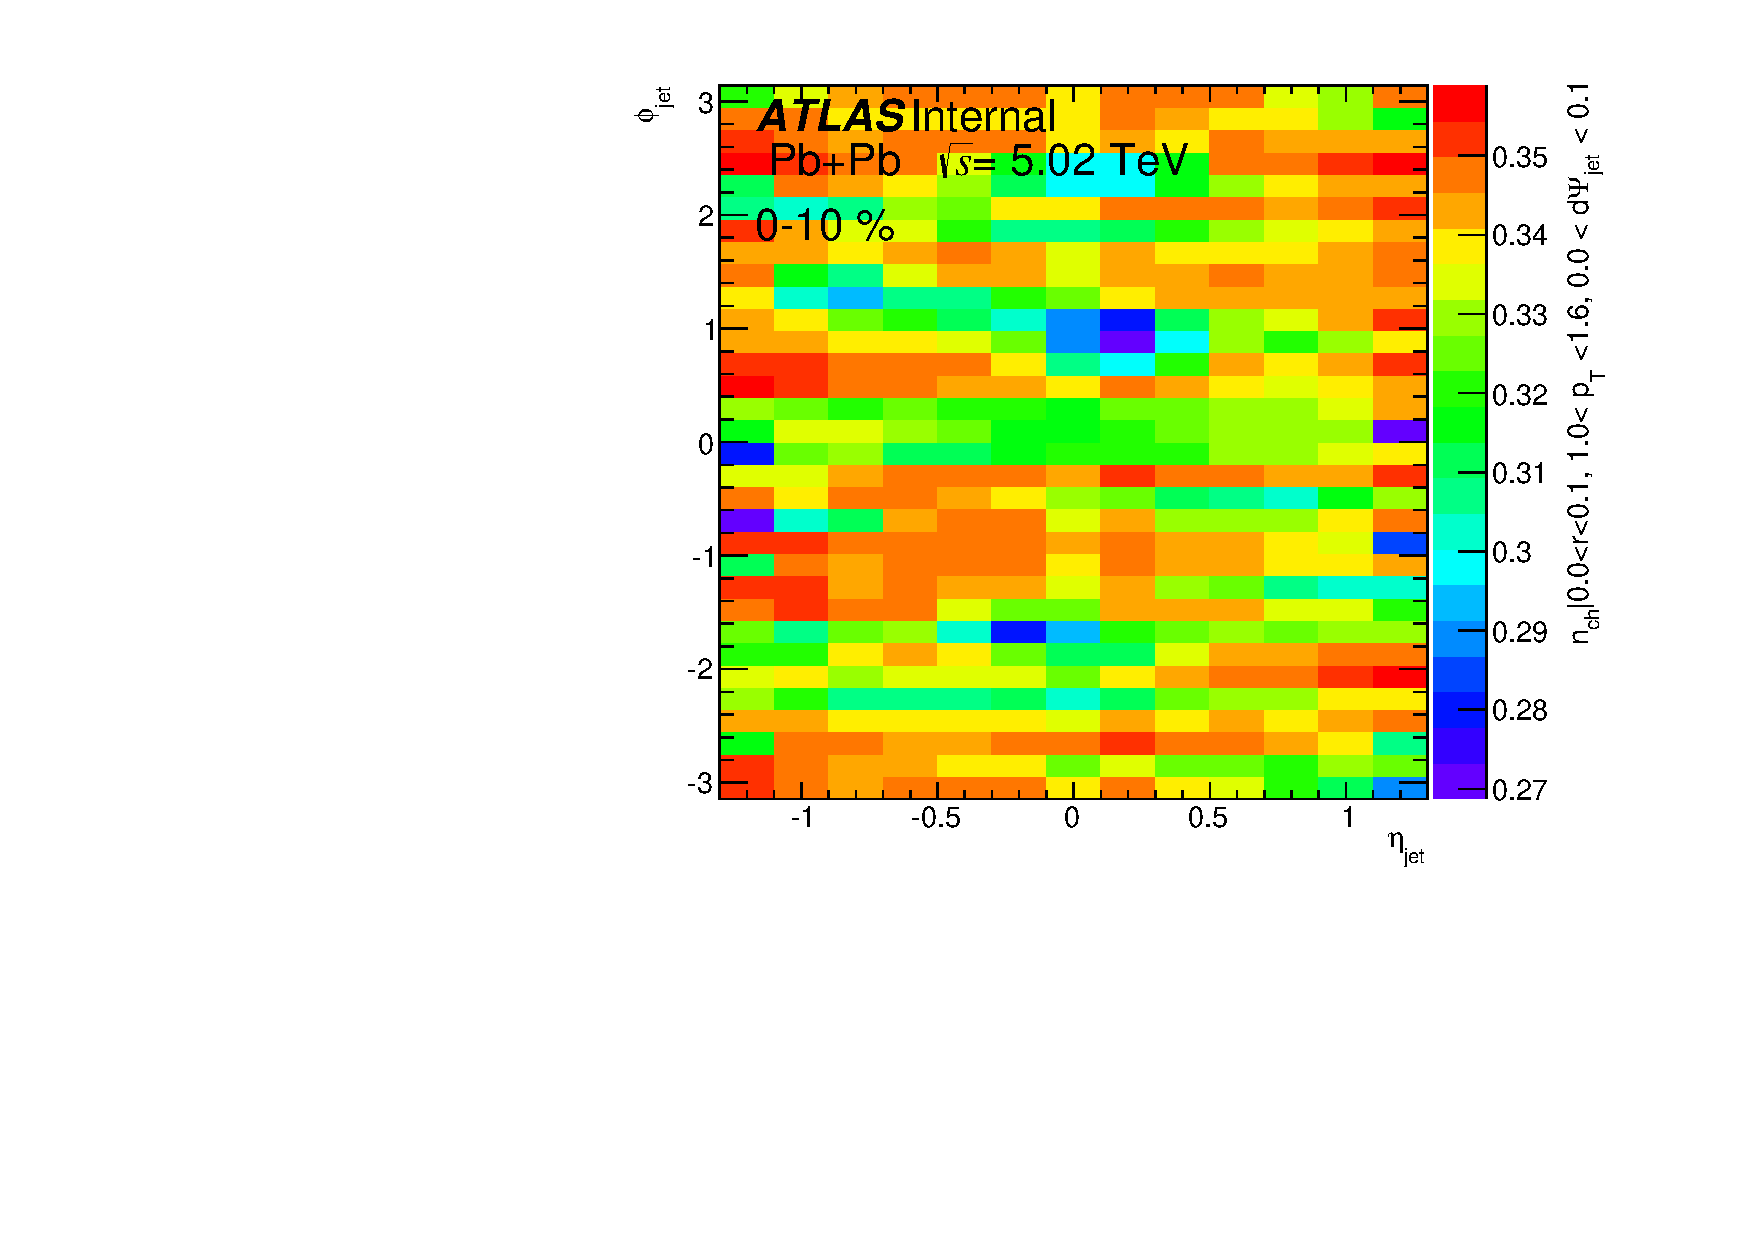
\includegraphics[width=0.33\textwidth]{figures_UE/h_UE_dR0_dPsi0_pt3_cent0.pdf} &
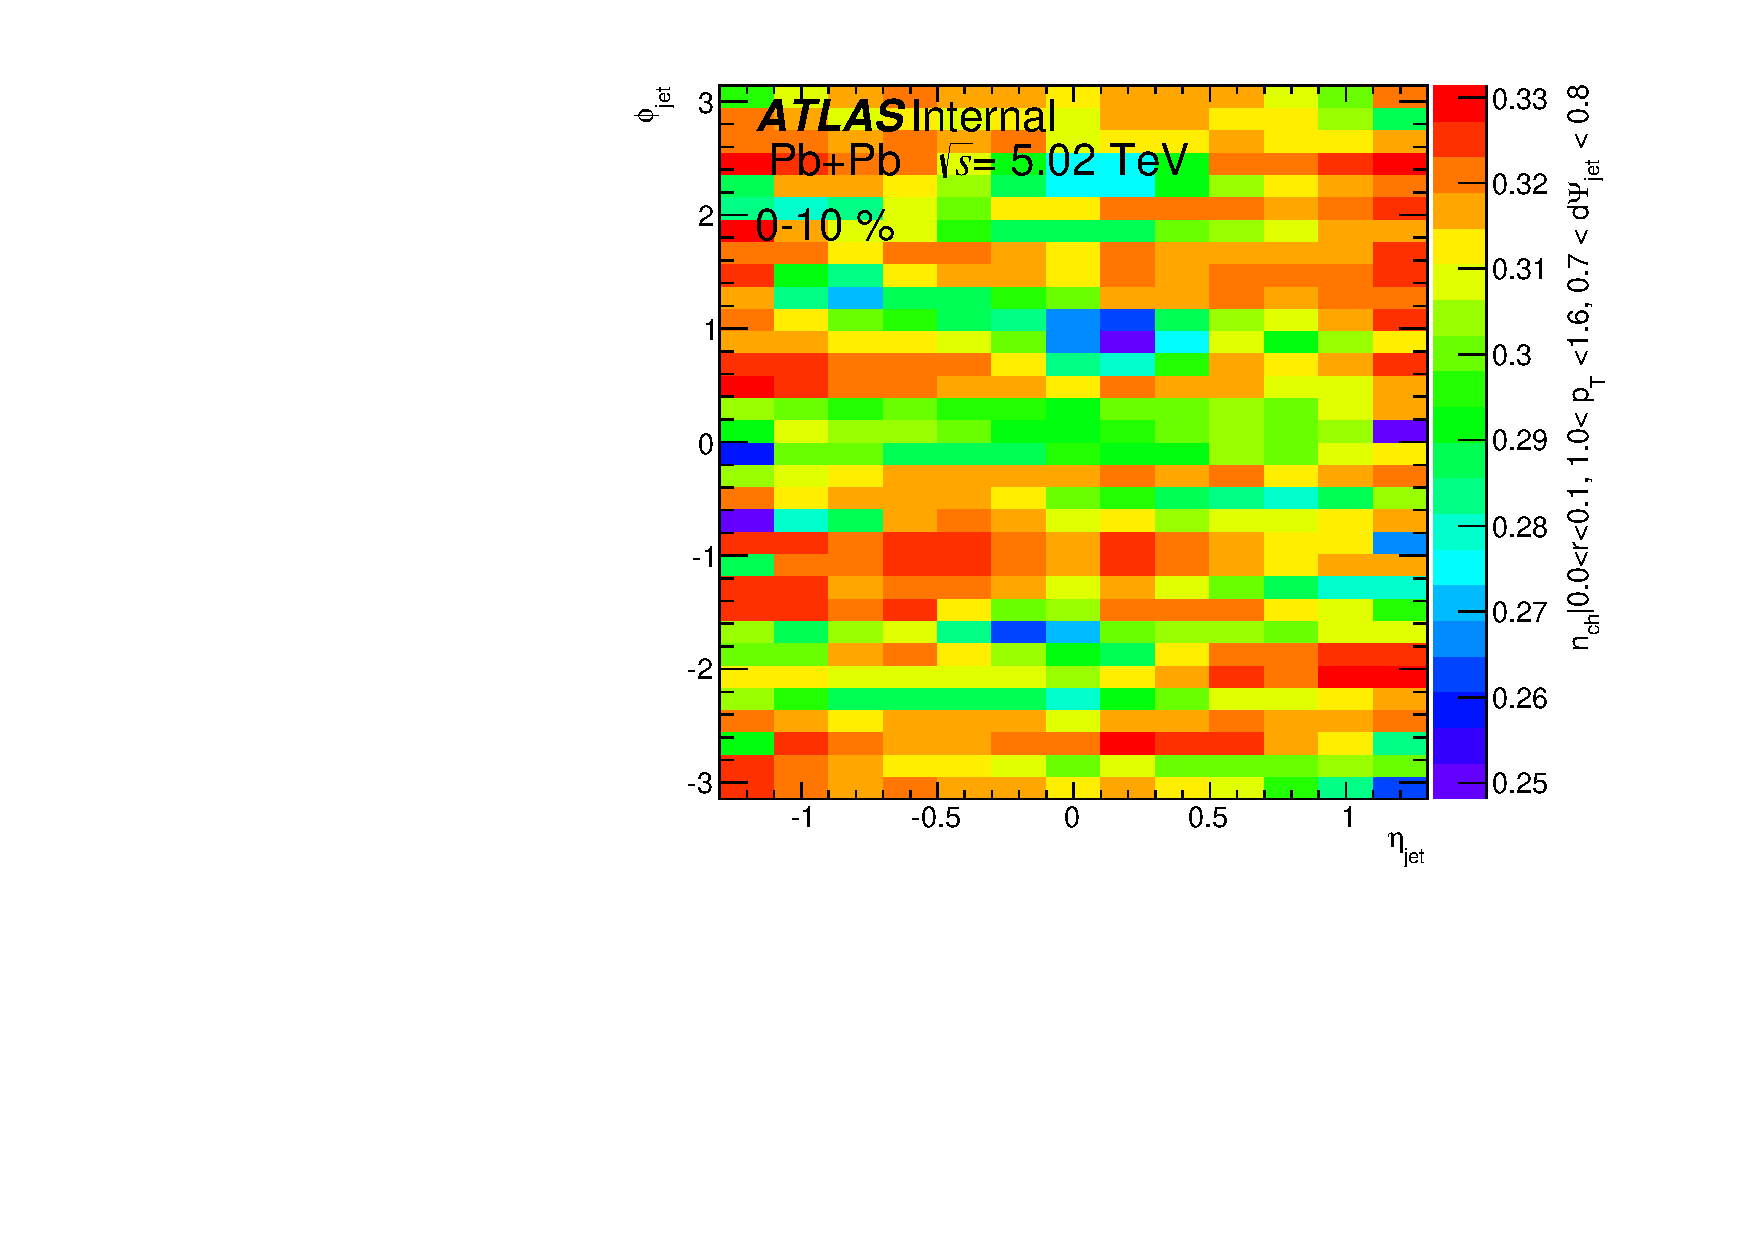
\includegraphics[width=0.33\textwidth]{figures_UE/h_UE_dR0_dPsi7_pt3_cent0.pdf}&
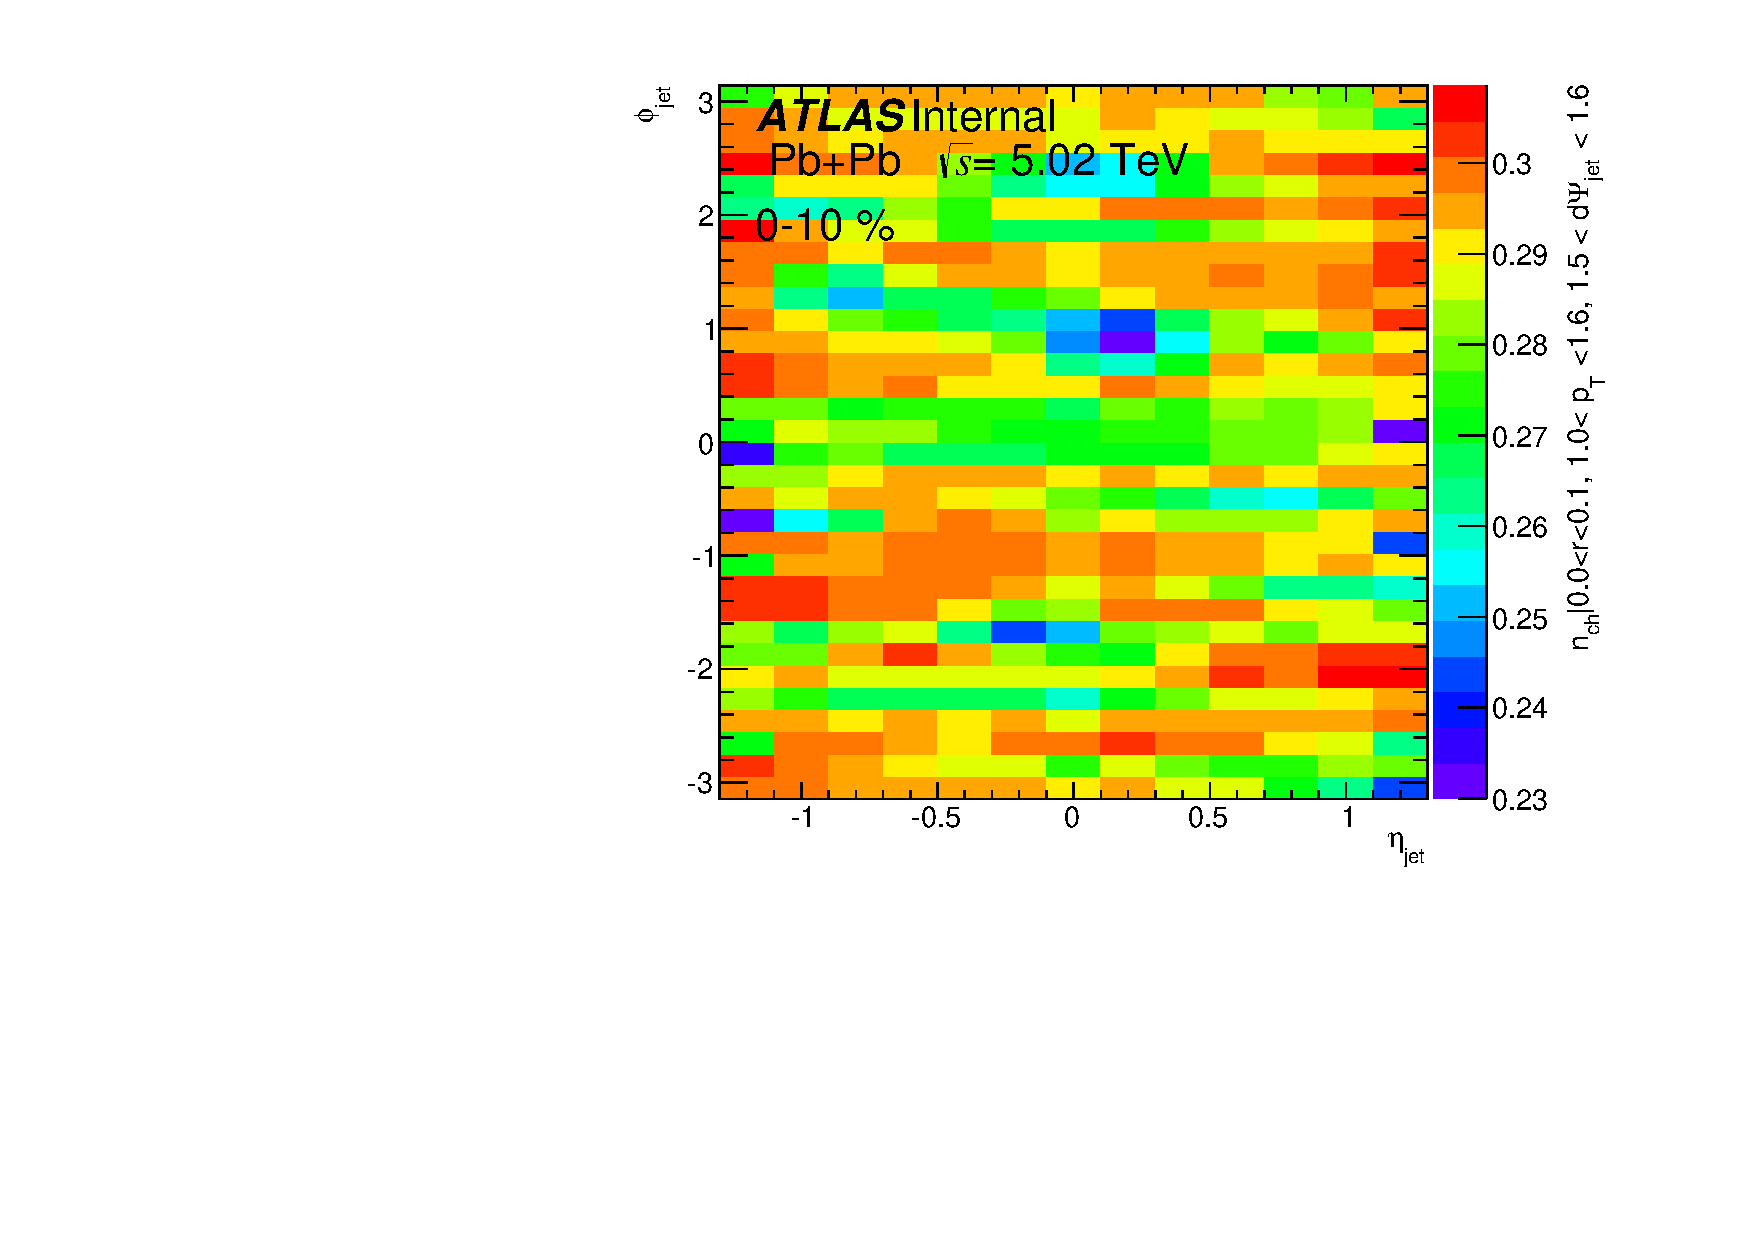
\includegraphics[width=0.33\textwidth]{figures_UE/h_UE_dR0_dPsi15_pt3_cent0.pdf} \\
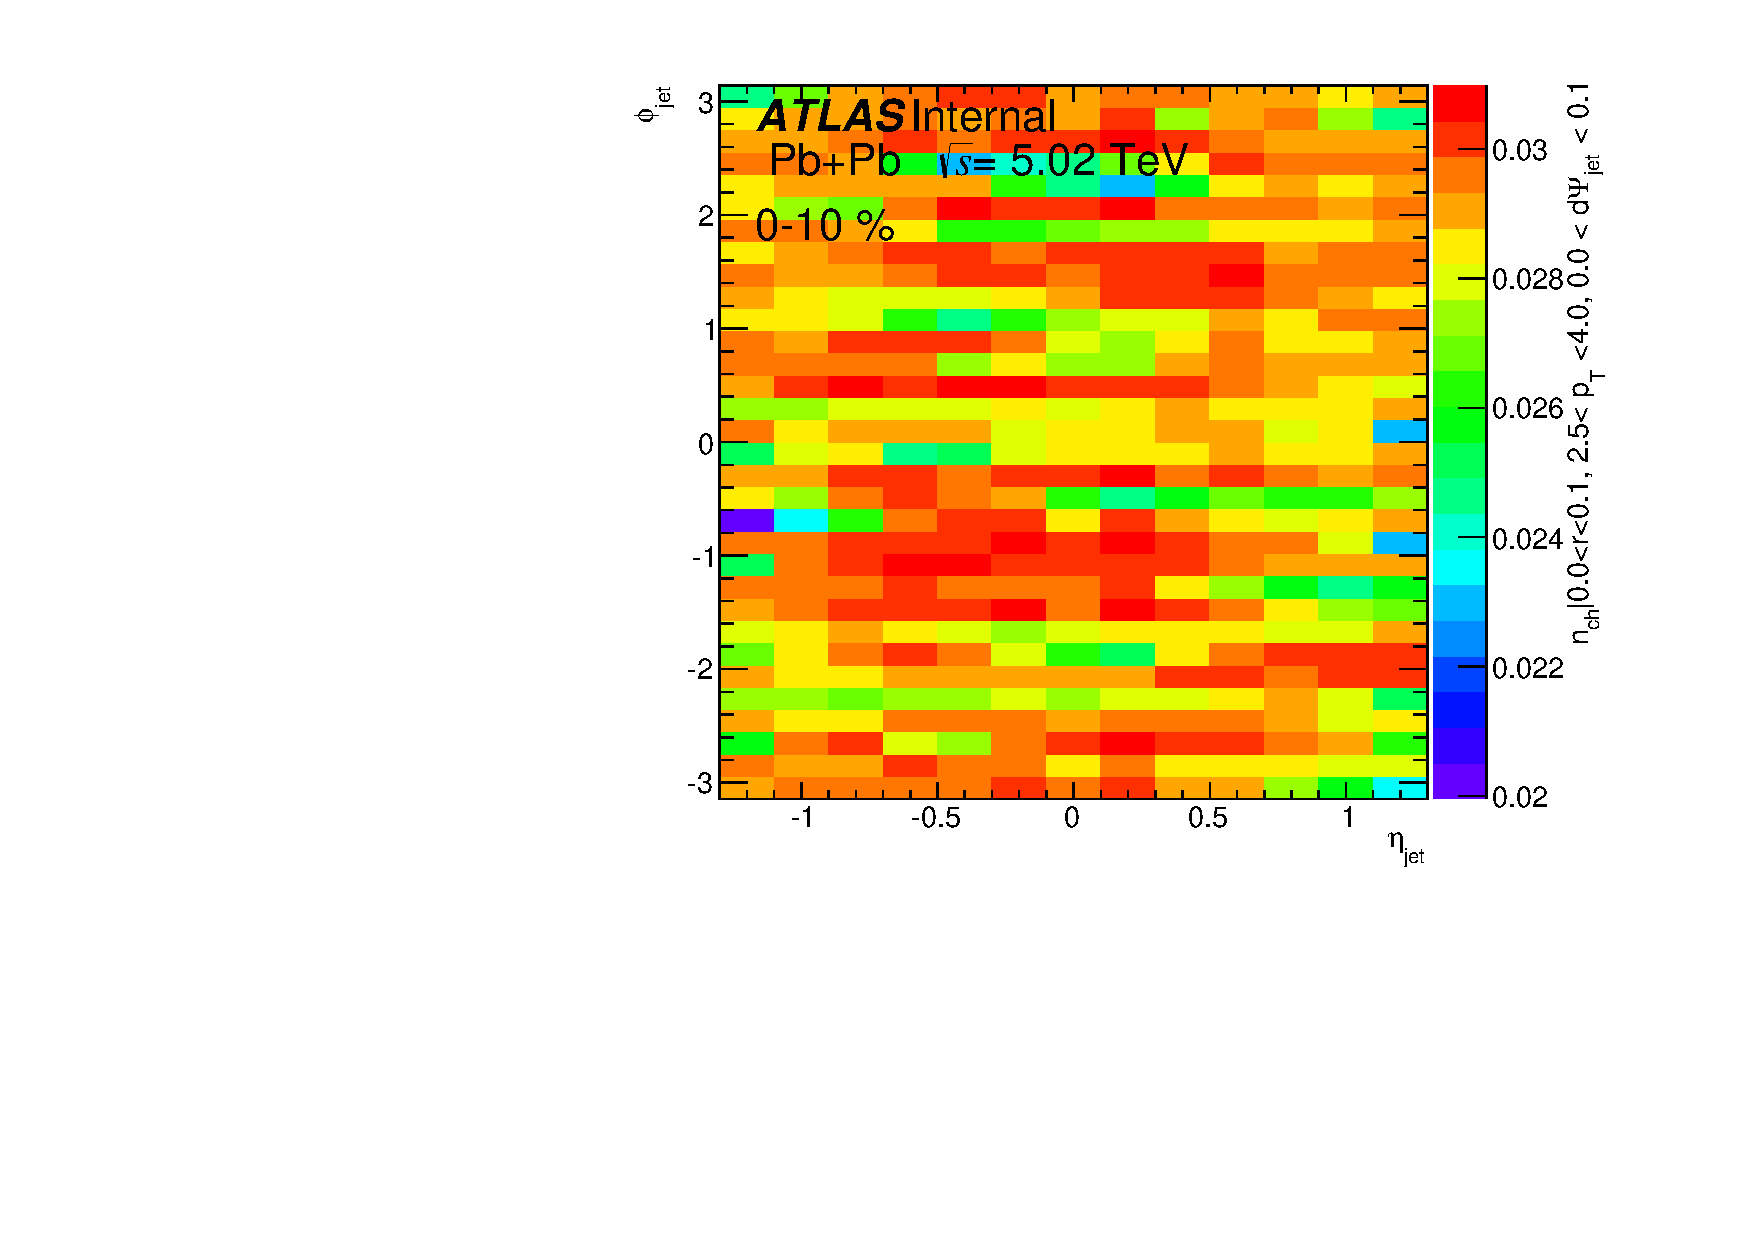
\includegraphics[width=0.33\textwidth]{figures_UE/h_UE_dR0_dPsi0_pt5_cent0.pdf} &
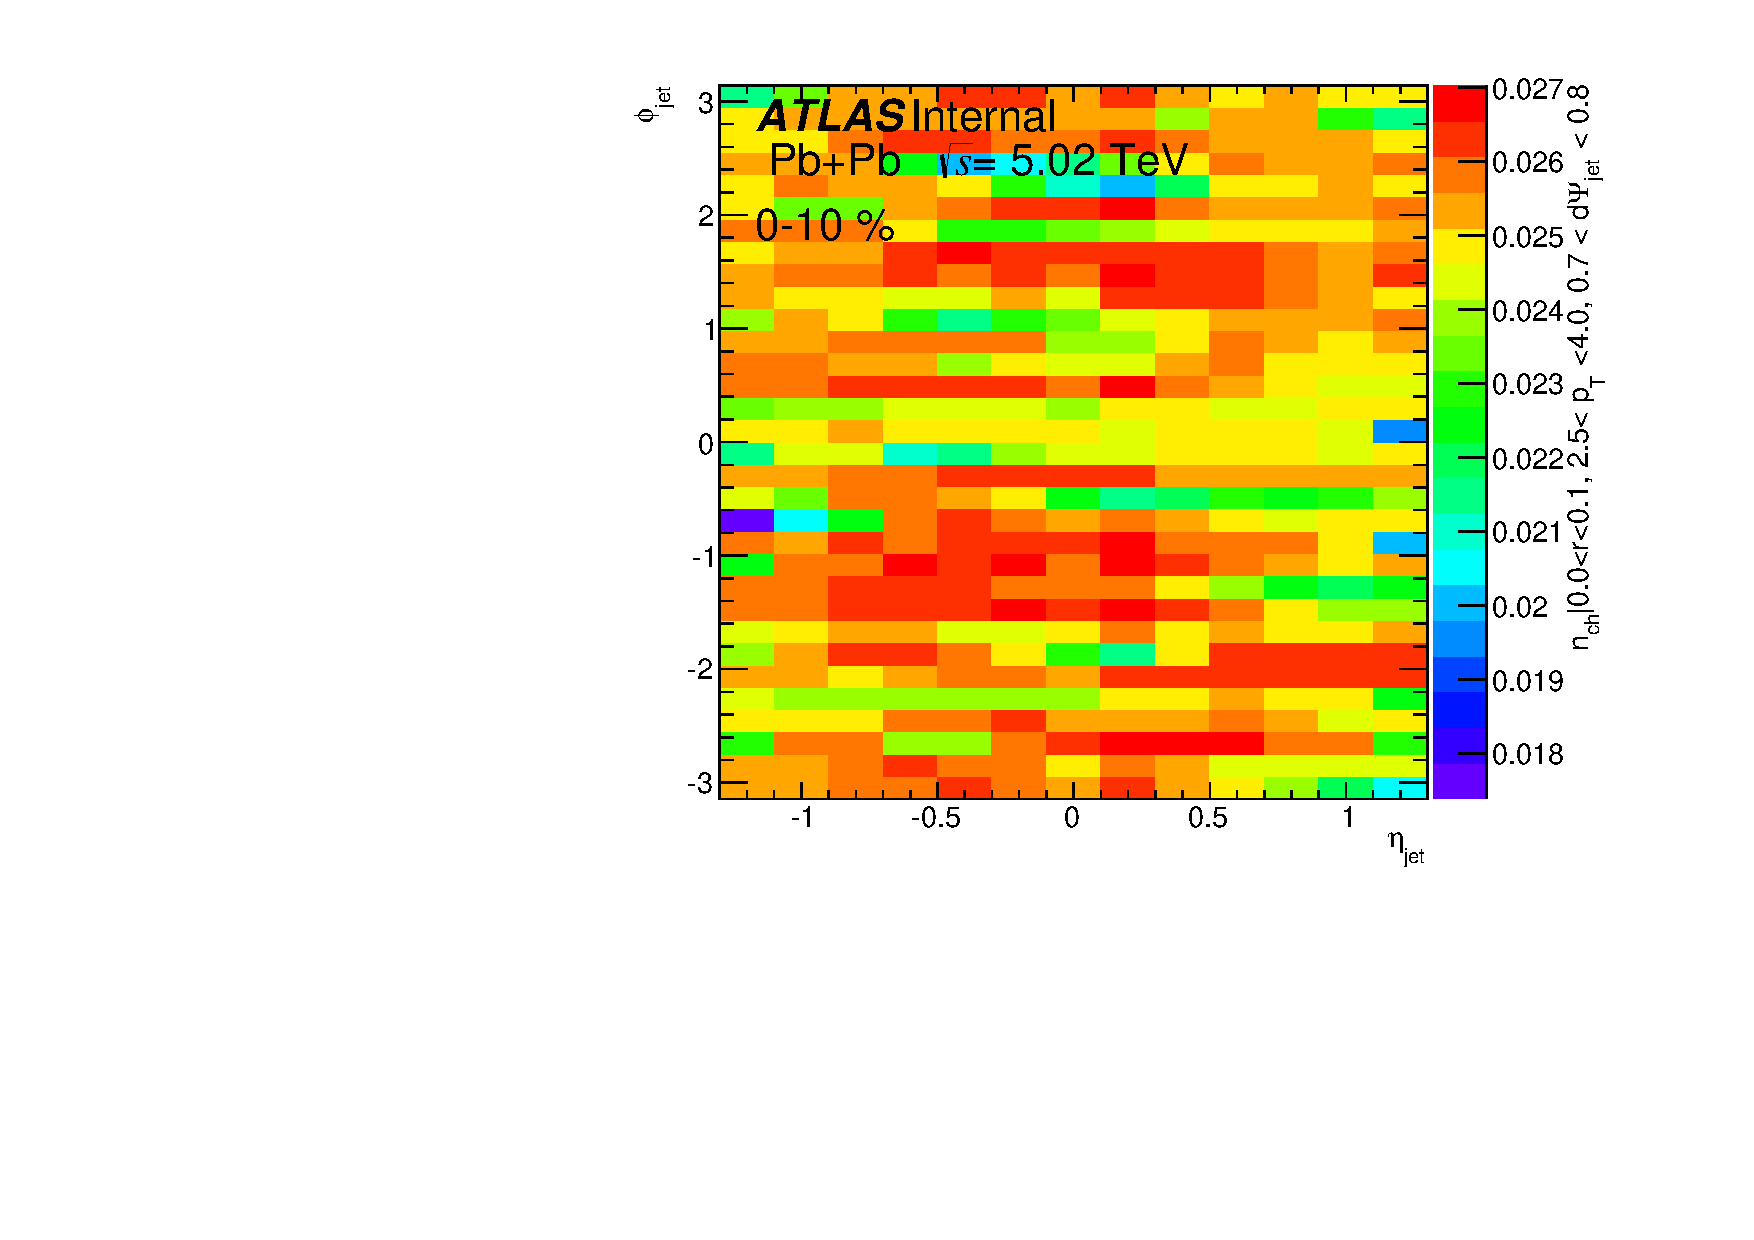
\includegraphics[width=0.33\textwidth]{figures_UE/h_UE_dR0_dPsi7_pt5_cent0.pdf}&
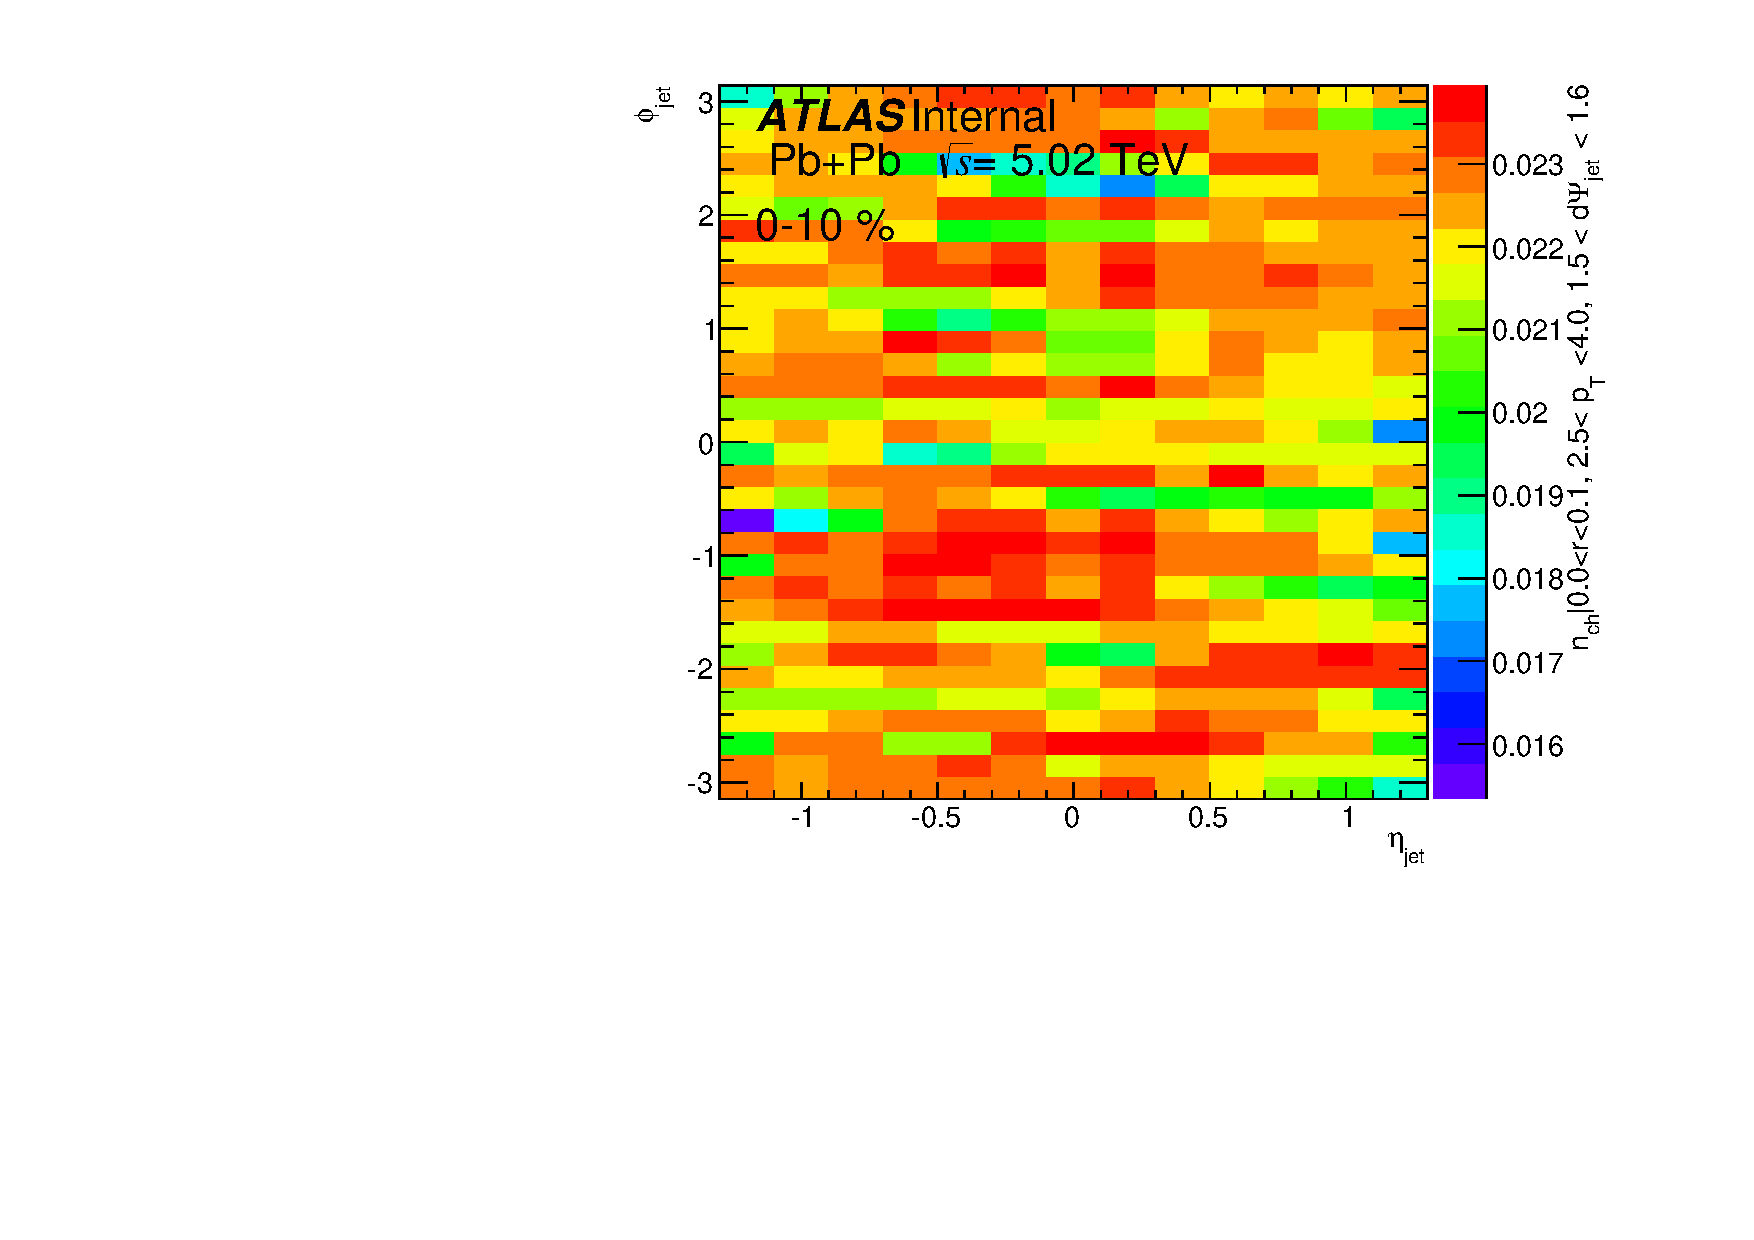
\includegraphics[width=0.33\textwidth]{figures_UE/h_UE_dR0_dPsi15_pt5_cent0.pdf} \\
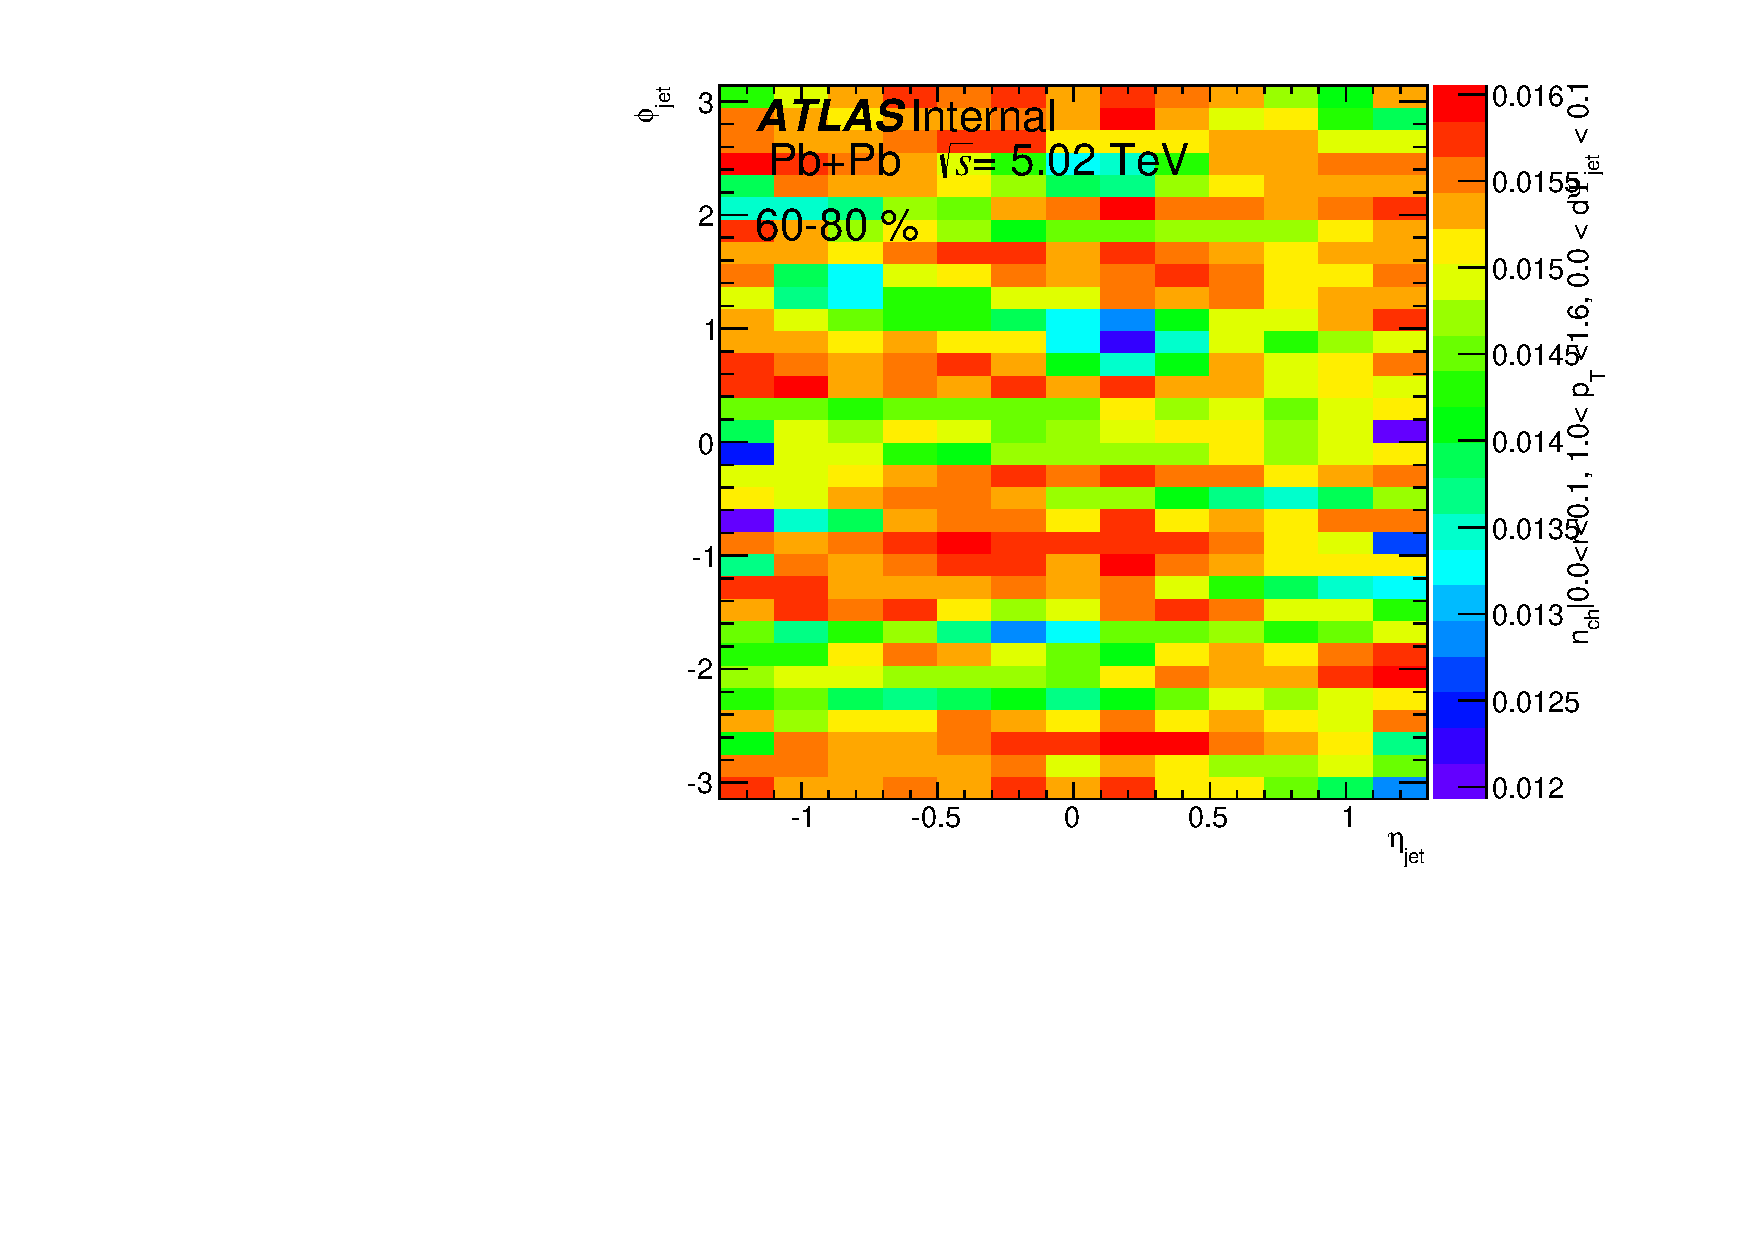
\includegraphics[width=0.33\textwidth]{figures_UE/h_UE_dR0_dPsi0_pt3_cent5.pdf} &
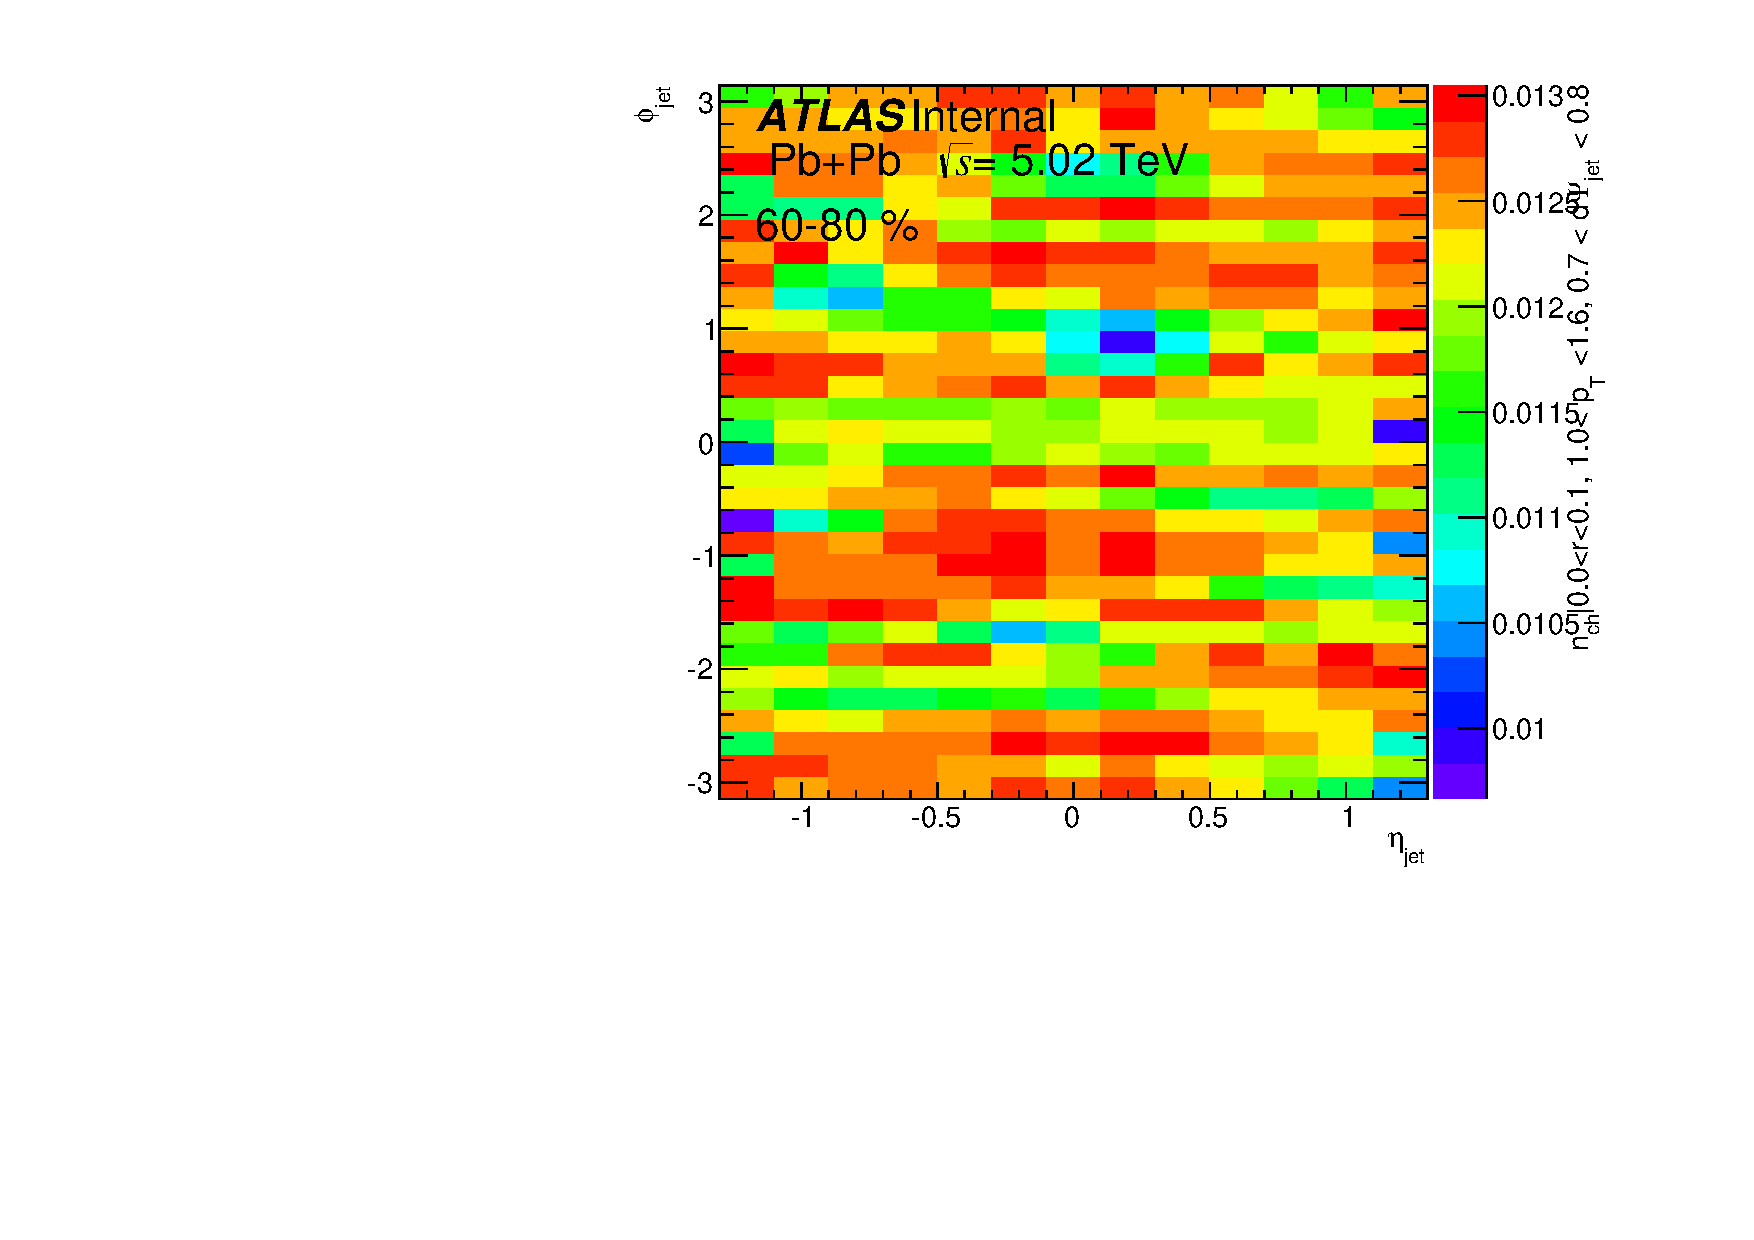
\includegraphics[width=0.33\textwidth]{figures_UE/h_UE_dR0_dPsi7_pt3_cent5.pdf}&
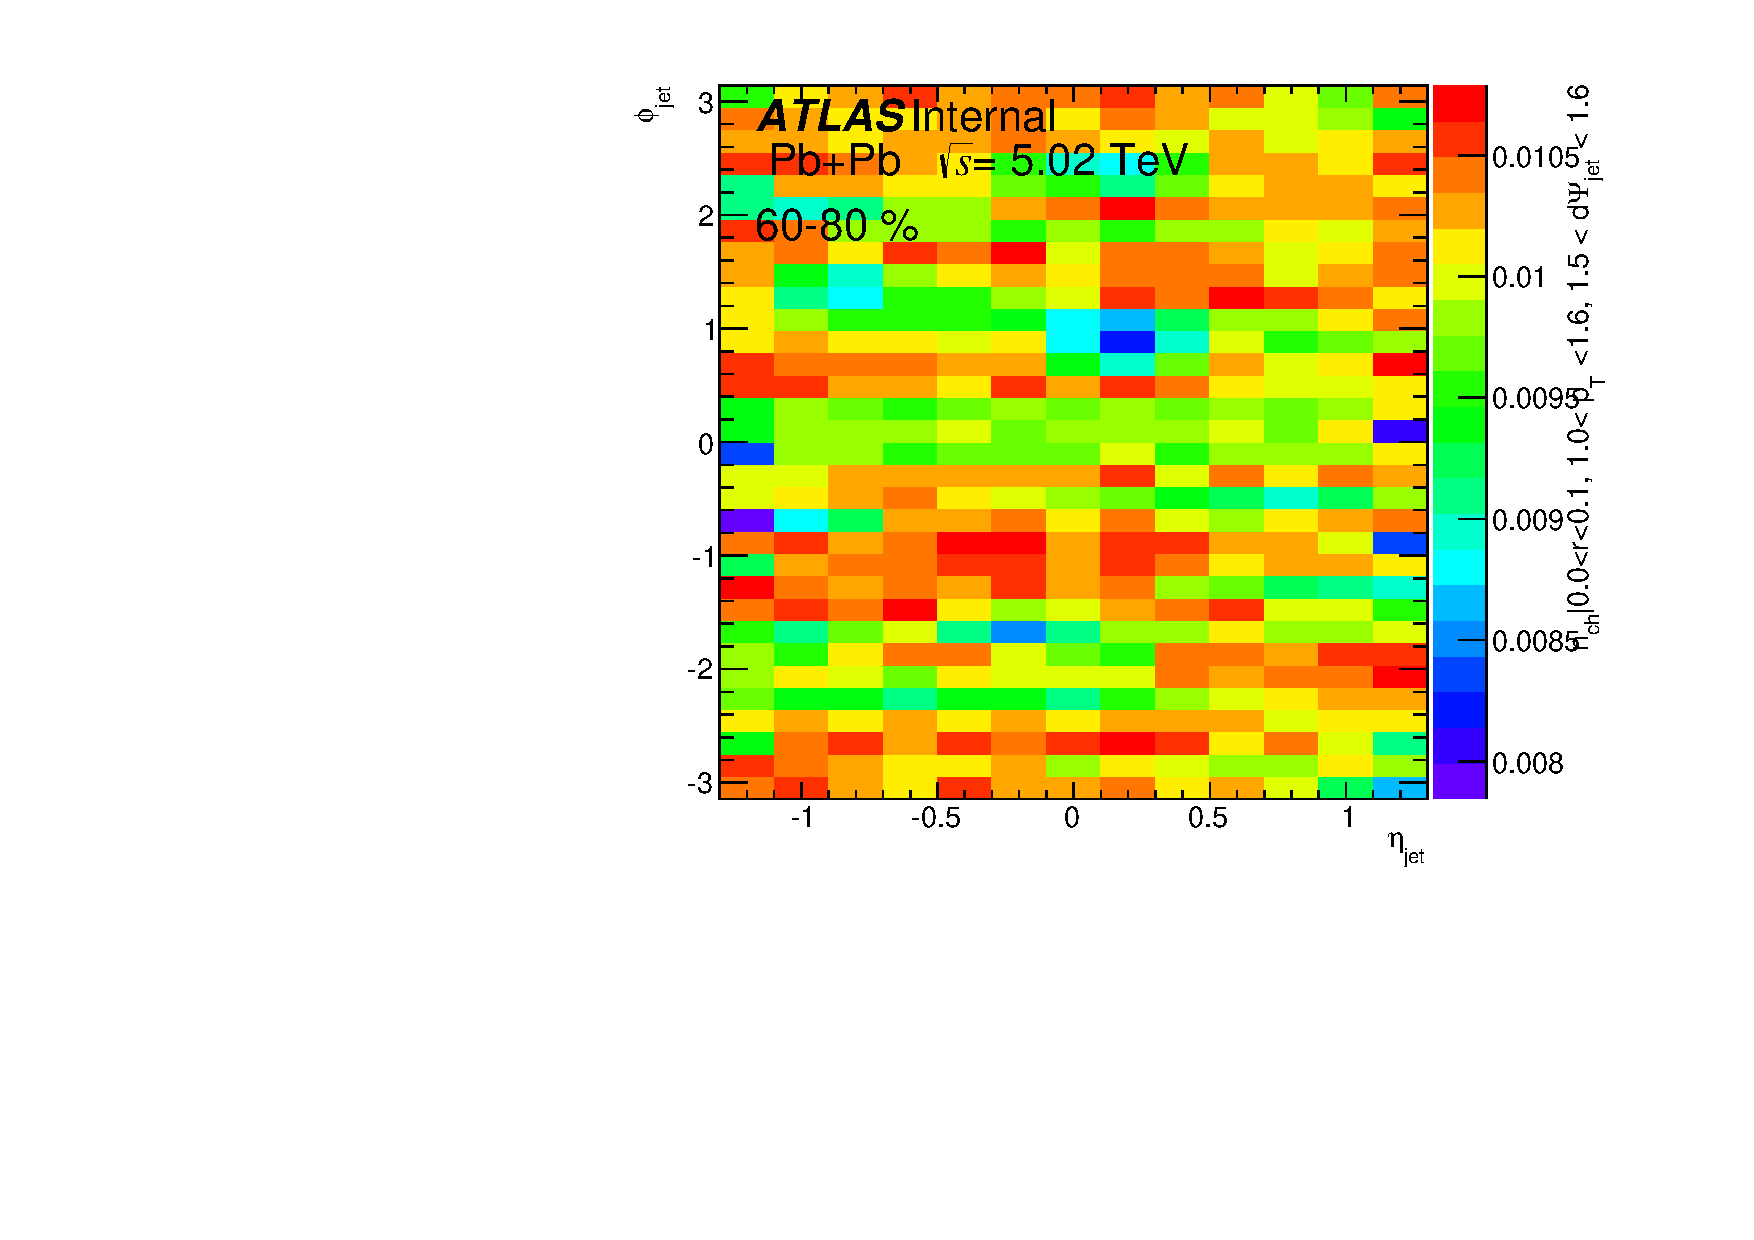
\includegraphics[width=0.33\textwidth]{figures_UE/h_UE_dR0_dPsi15_pt3_cent5.pdf} \\
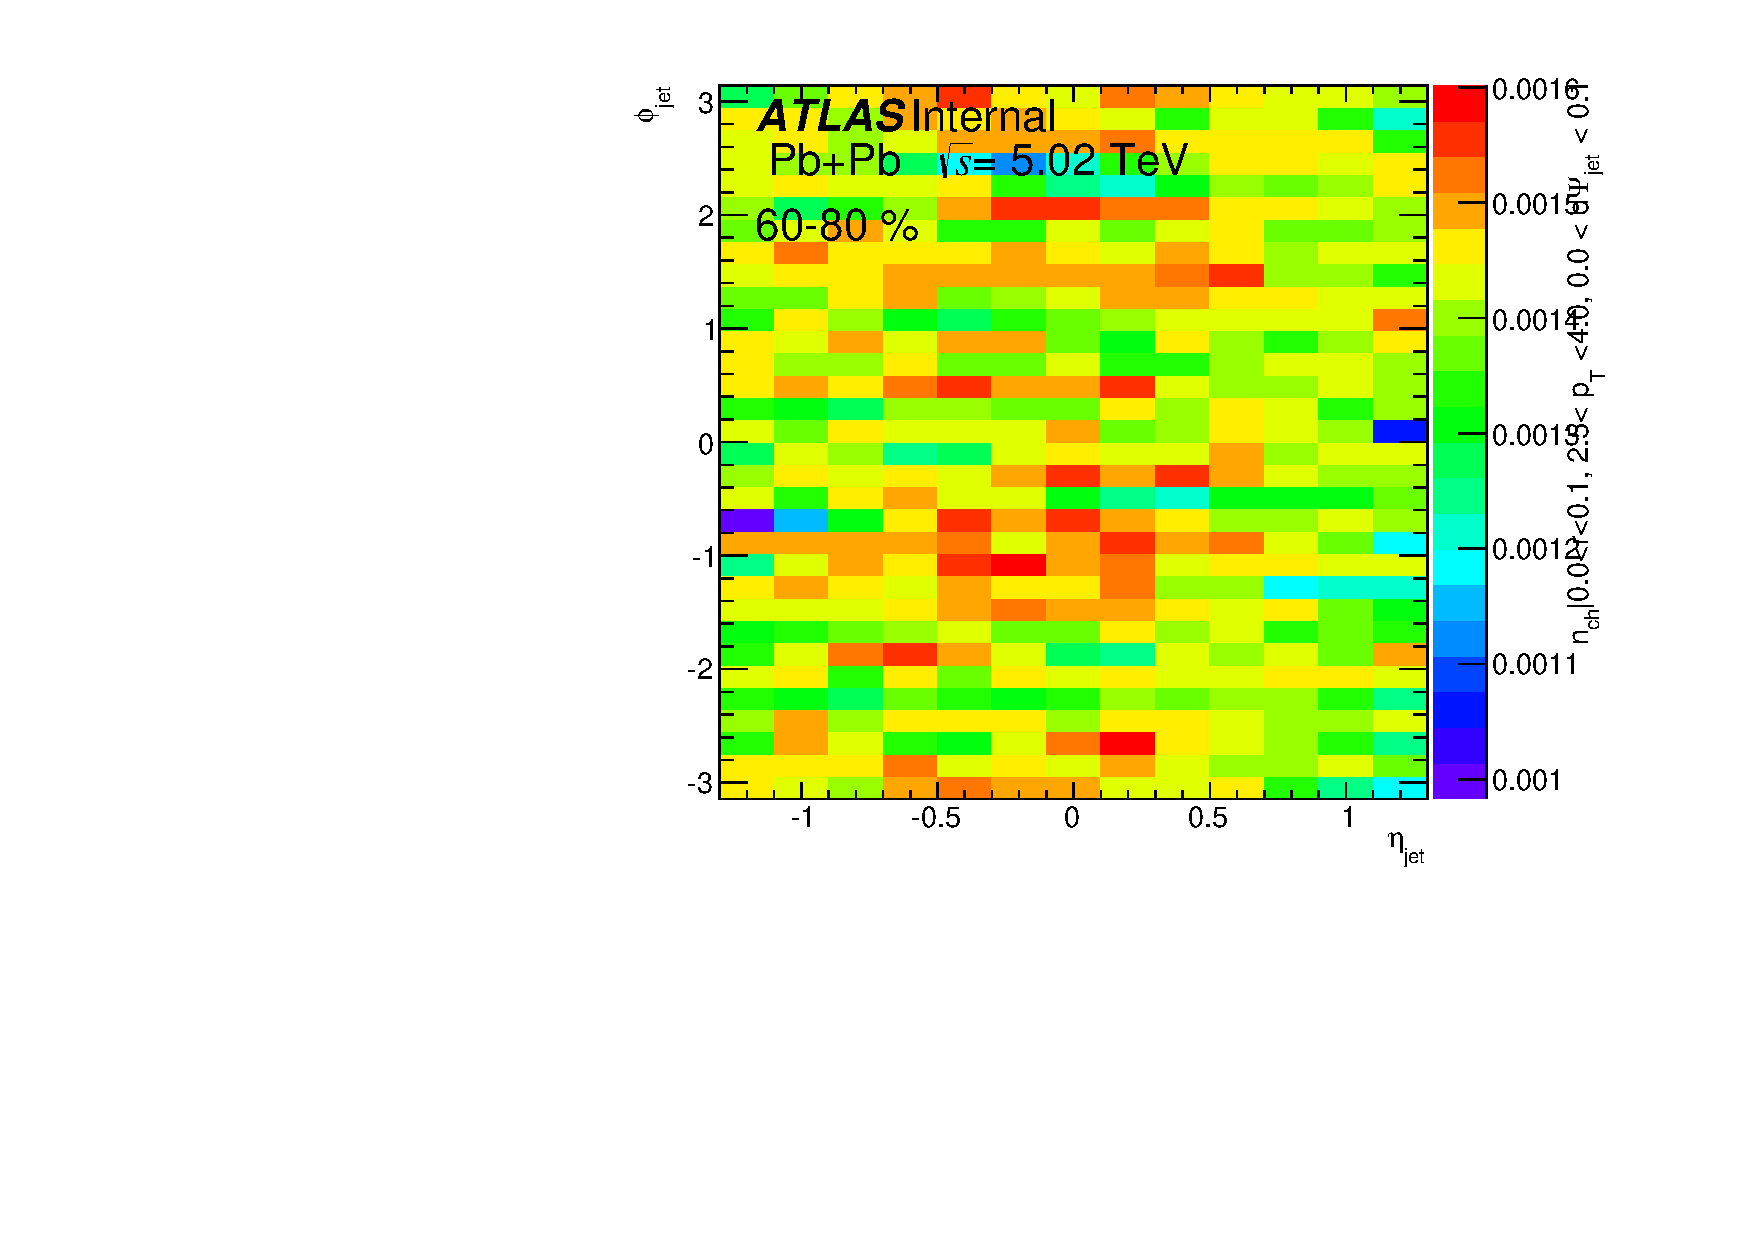
\includegraphics[width=0.33\textwidth]{figures_UE/h_UE_dR0_dPsi0_pt5_cent5.pdf} &
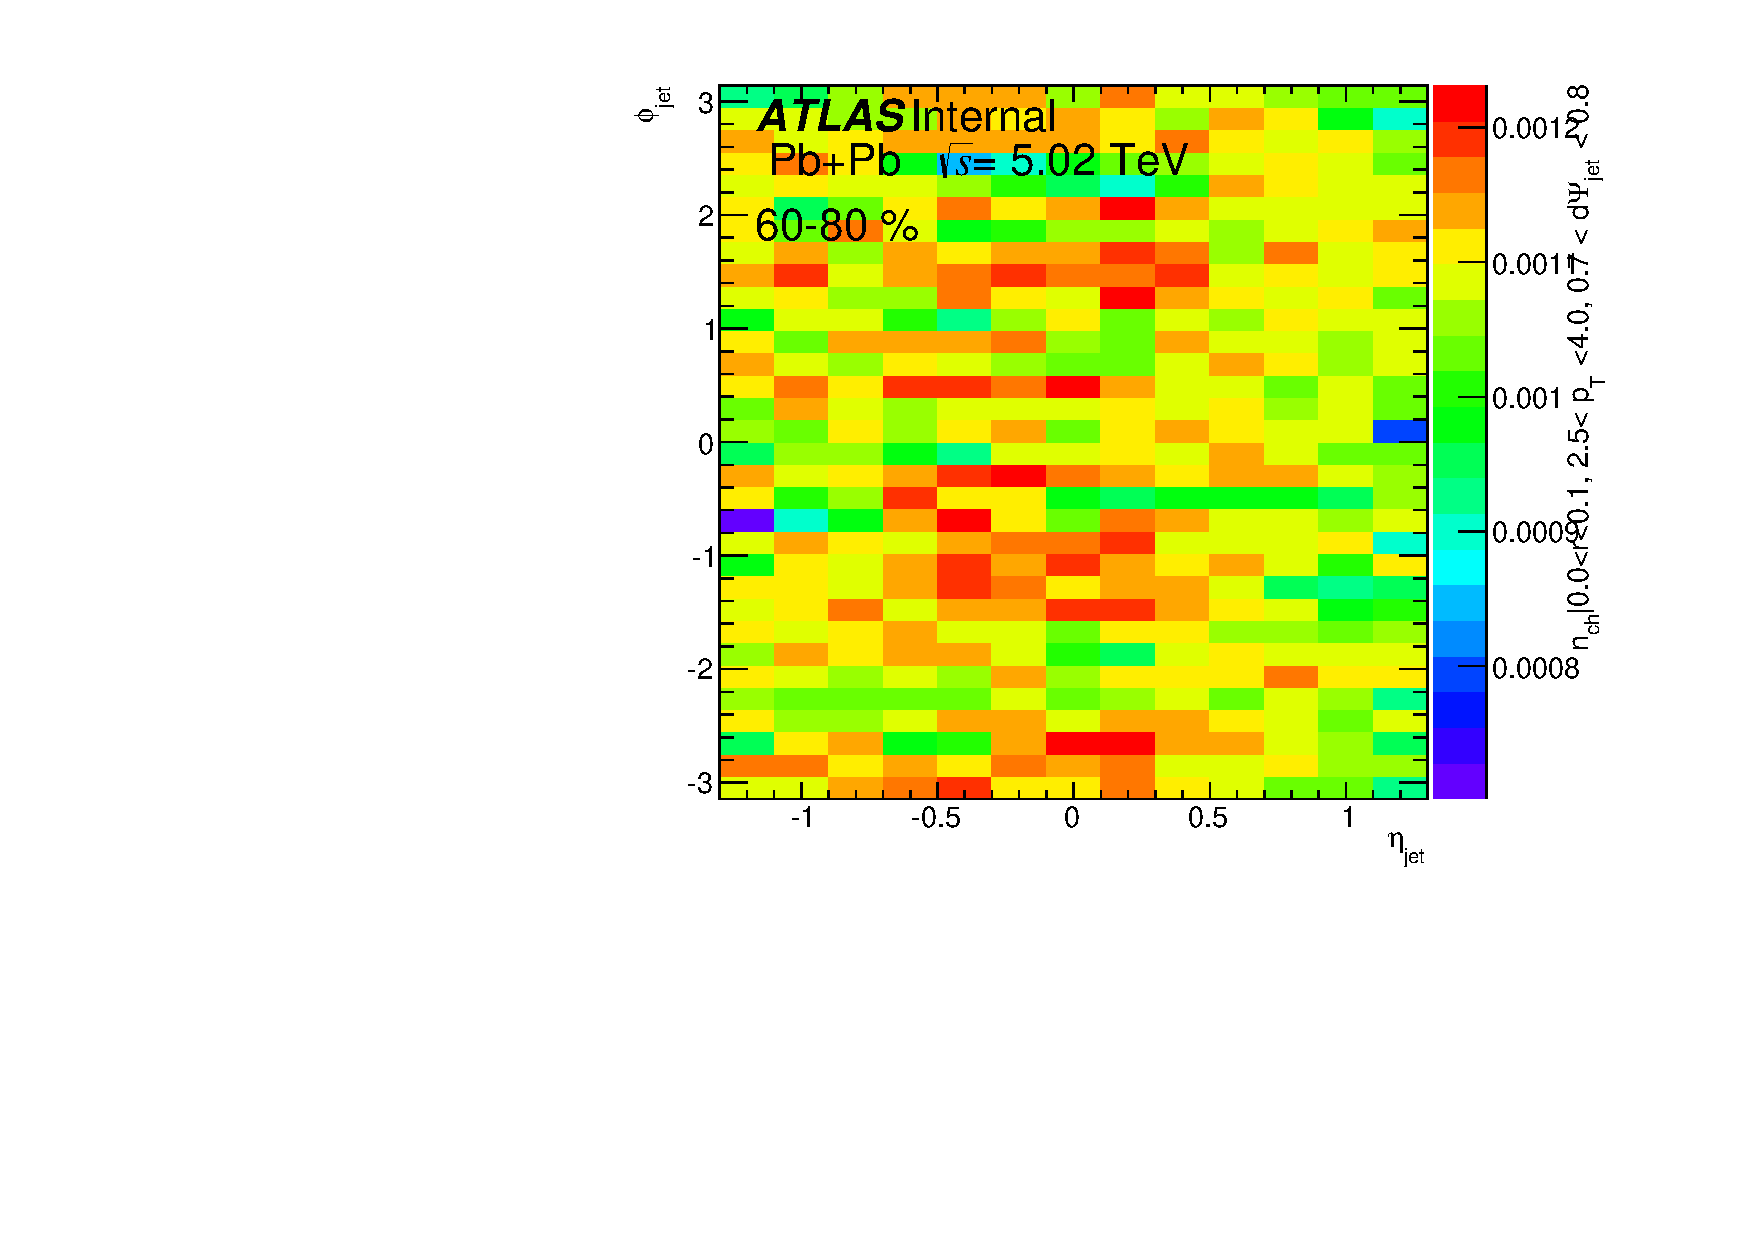
\includegraphics[width=0.33\textwidth]{figures_UE/h_UE_dR0_dPsi7_pt5_cent5.pdf}&
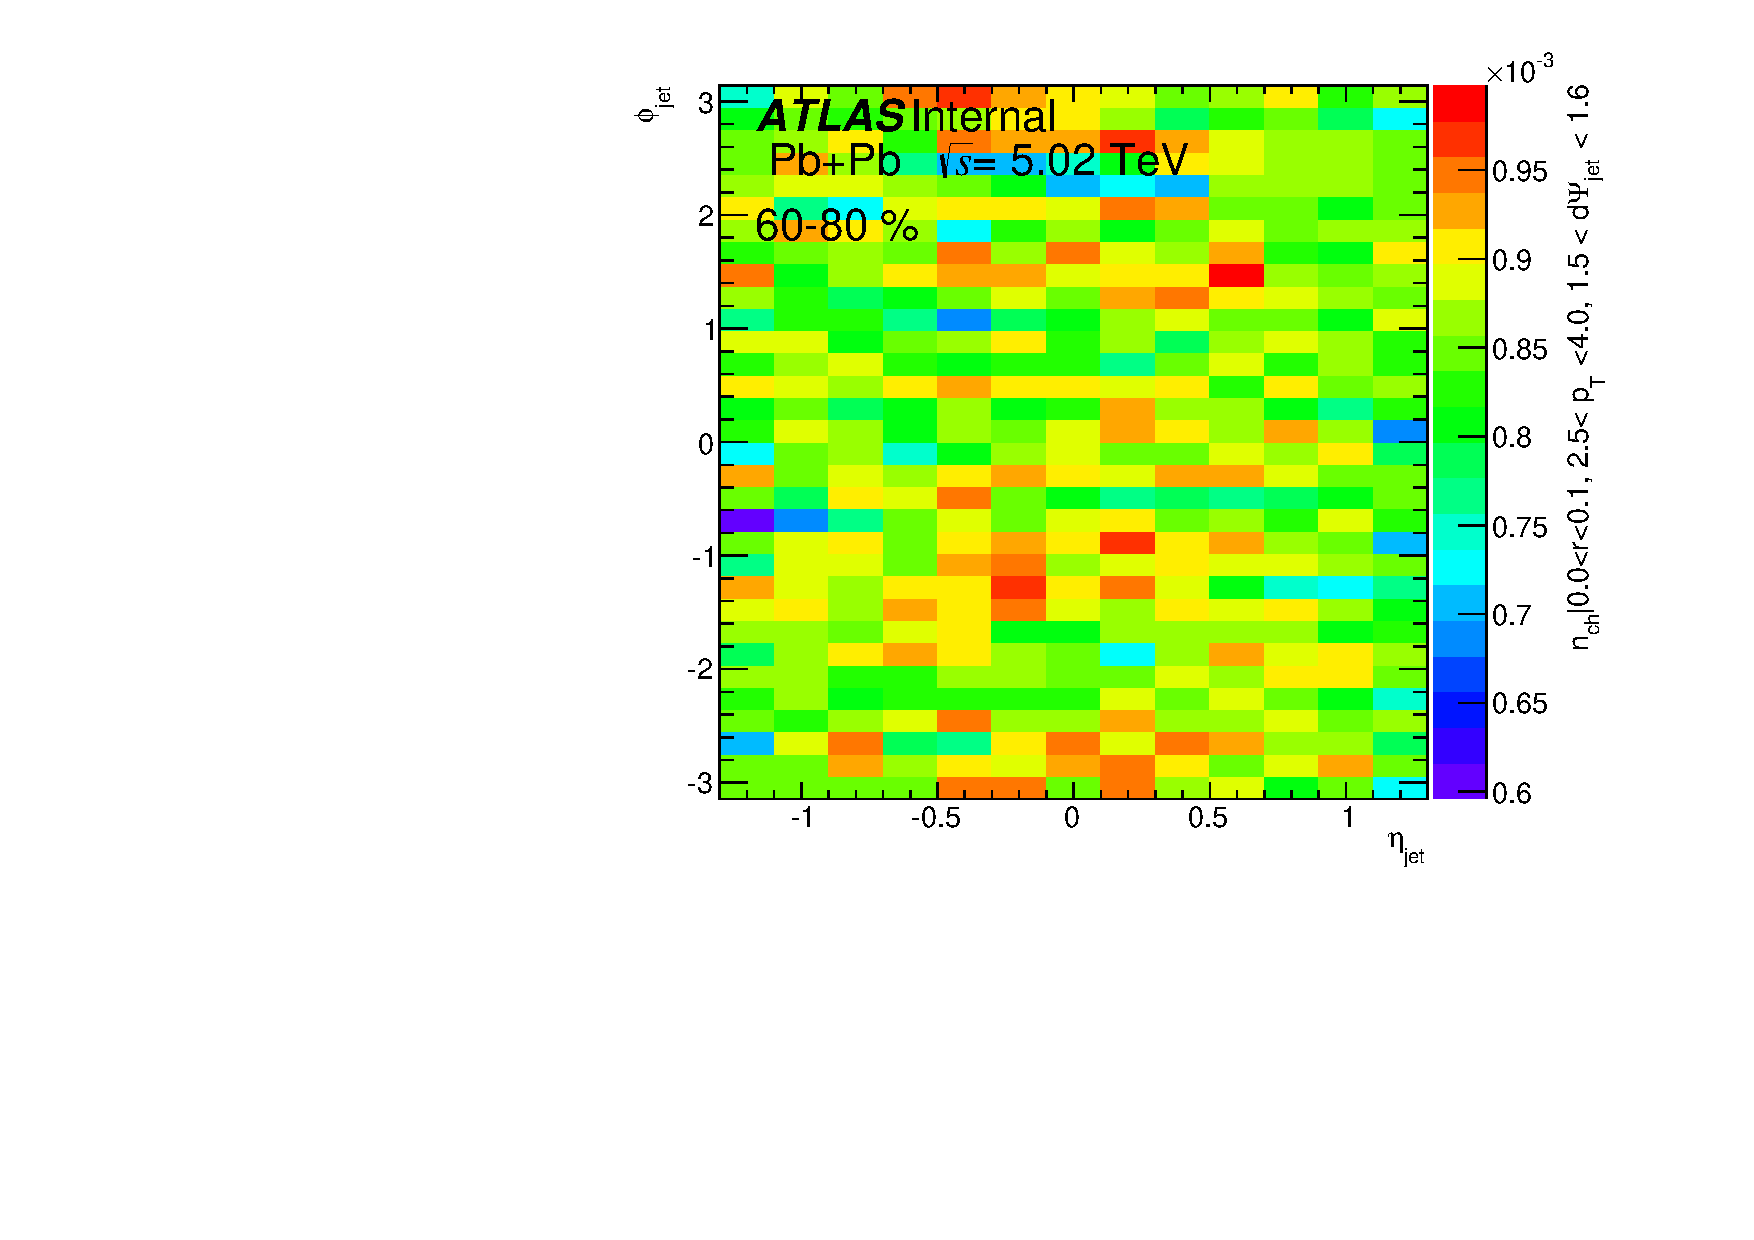
\includegraphics[width=0.33\textwidth]{figures_UE/h_UE_dR0_dPsi15_pt5_cent5.pdf} \\
\end{tabular}}
\caption{
Per jet $\nchUE^{\mathrm{MB}}$ distributions of charged particles evaluated in the core of the jet ($0.<r<0.05$) in MB events in three different intervals of angular distance with respect to the reaction plane angle going from left to right for two different selection of charged particle \pt\ and for two different centrality intervals.}
\label{fig:nchcore1}
\end{figure}

\begin{figure}[ht]
\centerline{
\begin{tabular}{ccc}
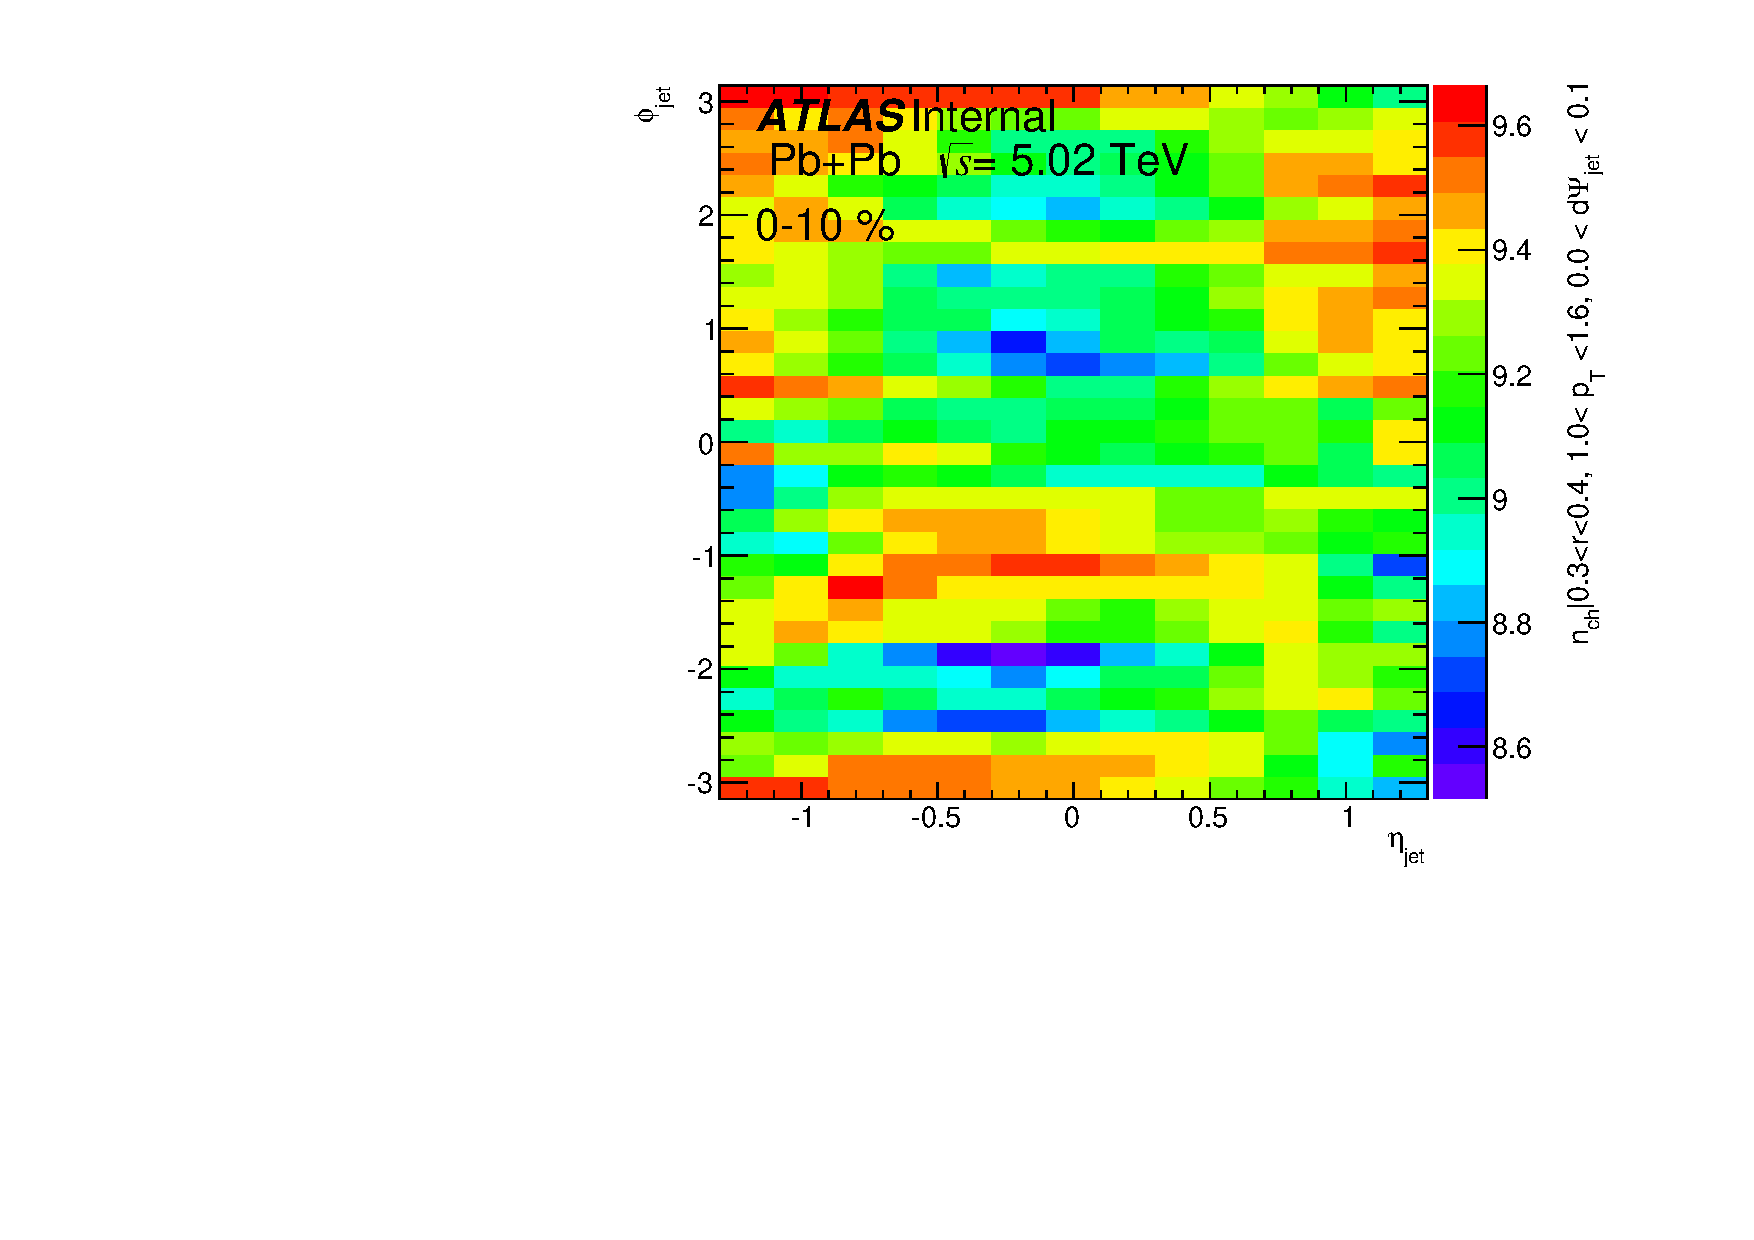
\includegraphics[width=0.33\textwidth]{figures_UE/h_UE_dR6_dPsi0_pt3_cent0.pdf} &
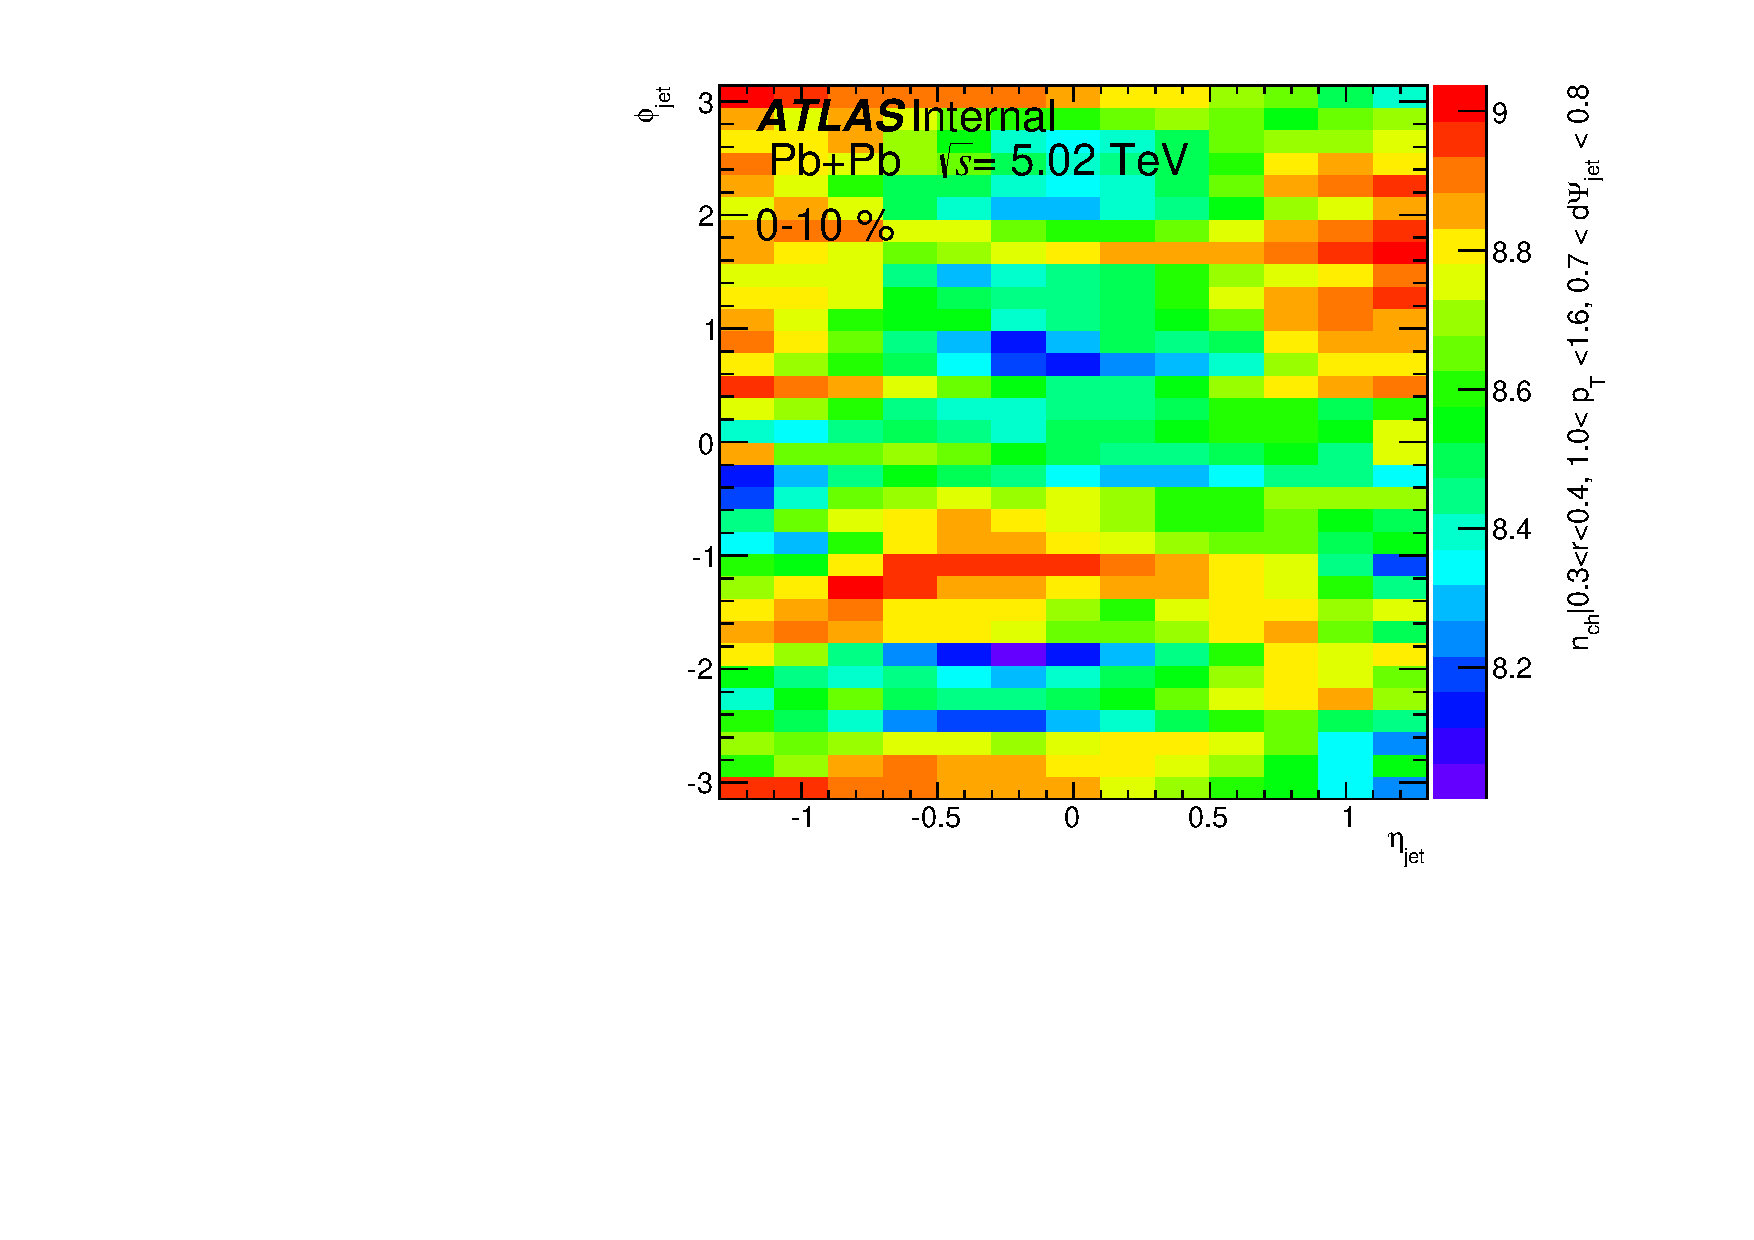
\includegraphics[width=0.33\textwidth]{figures_UE/h_UE_dR6_dPsi7_pt3_cent0.pdf}&
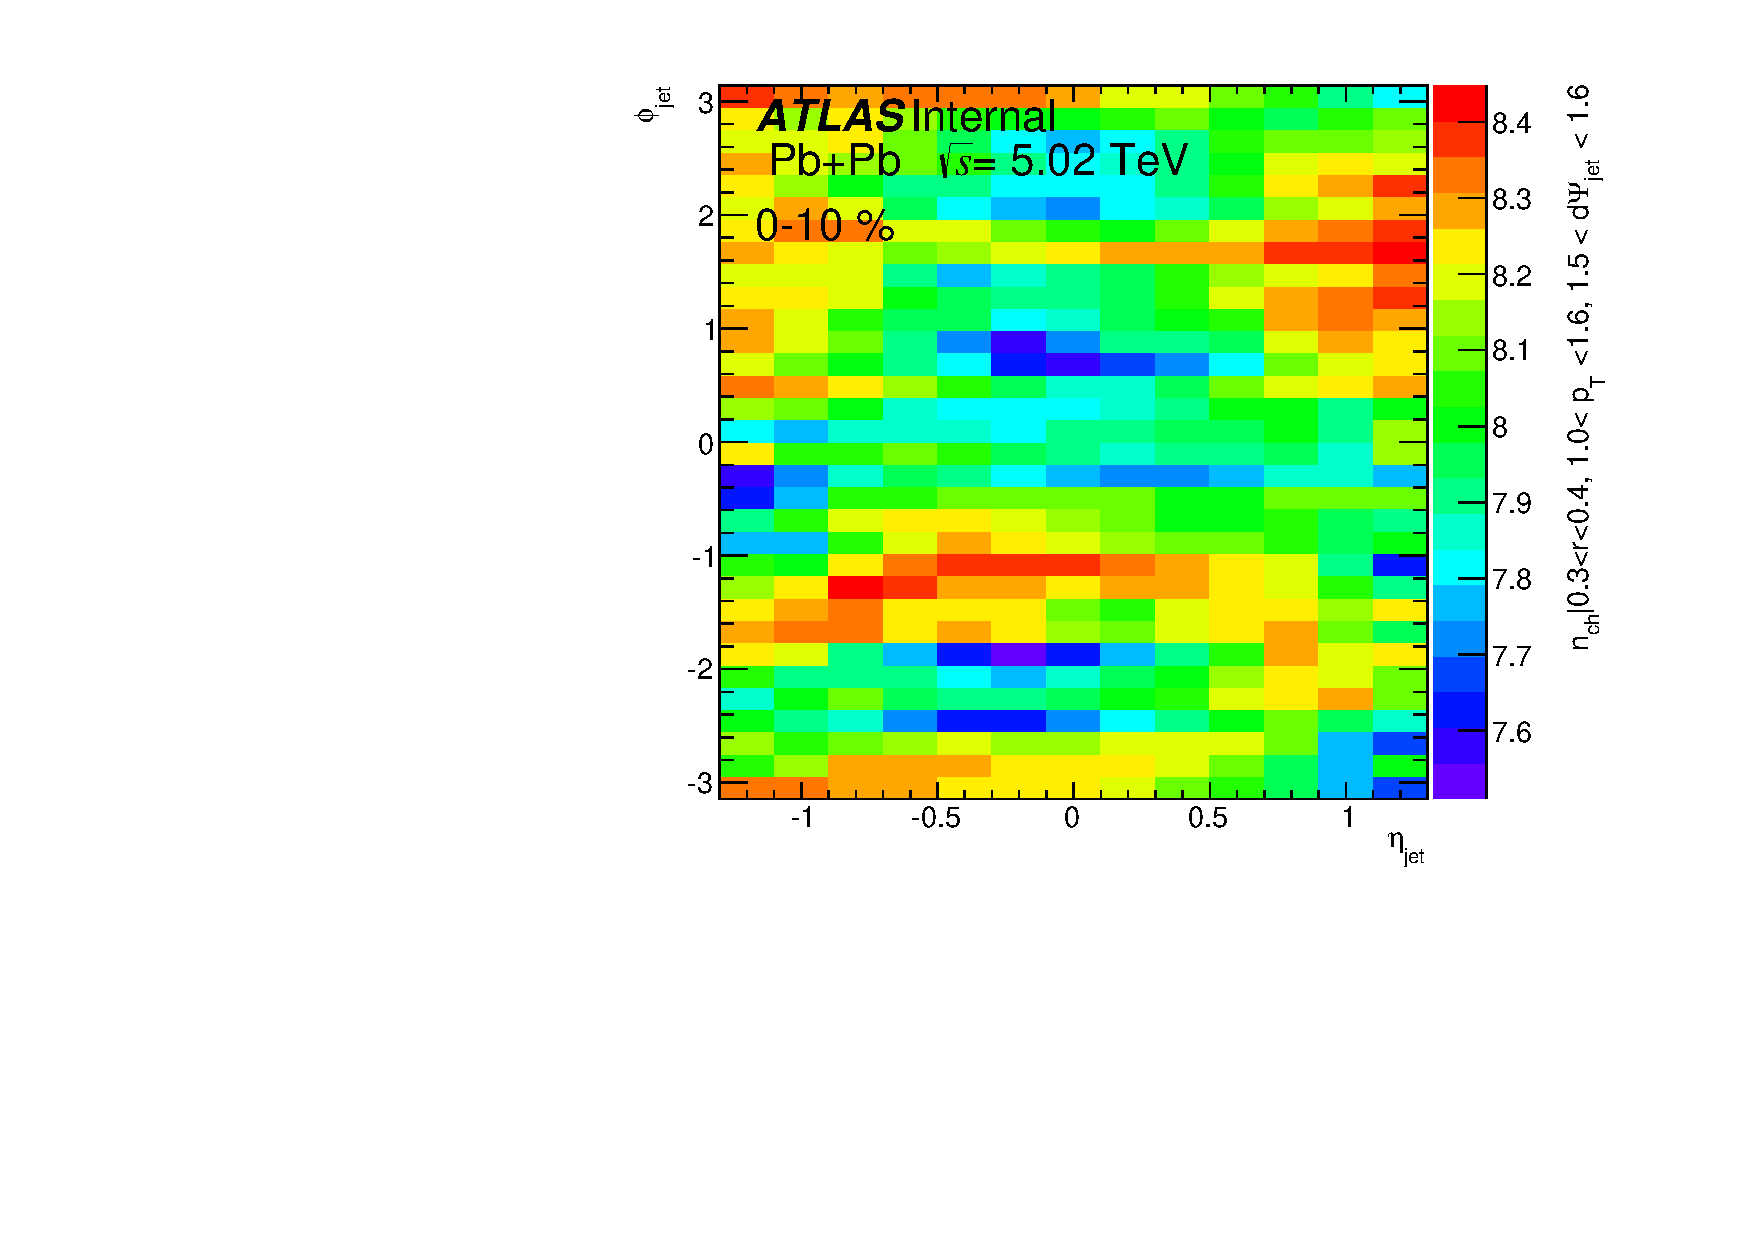
\includegraphics[width=0.33\textwidth]{figures_UE/h_UE_dR6_dPsi15_pt3_cent0.pdf} \\
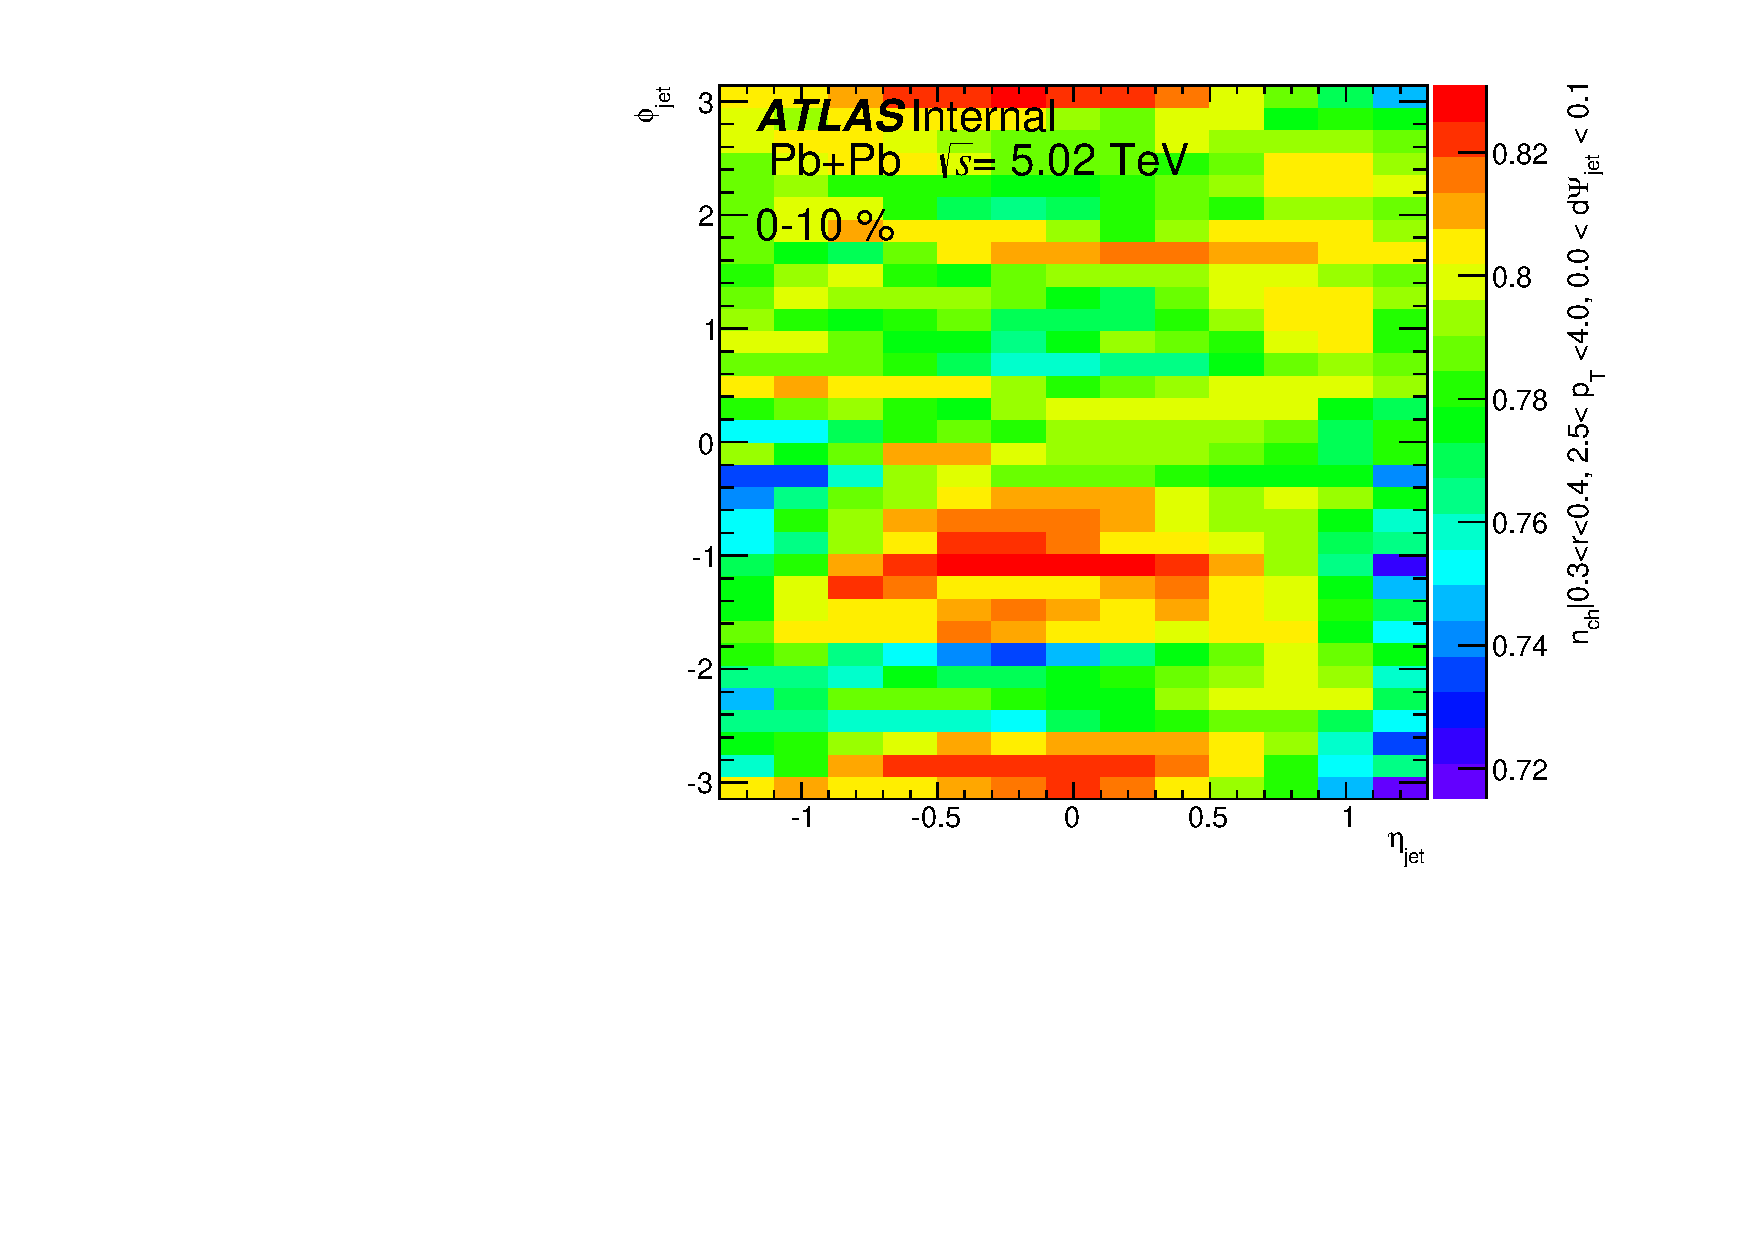
\includegraphics[width=0.33\textwidth]{figures_UE/h_UE_dR6_dPsi0_pt5_cent0.pdf} &
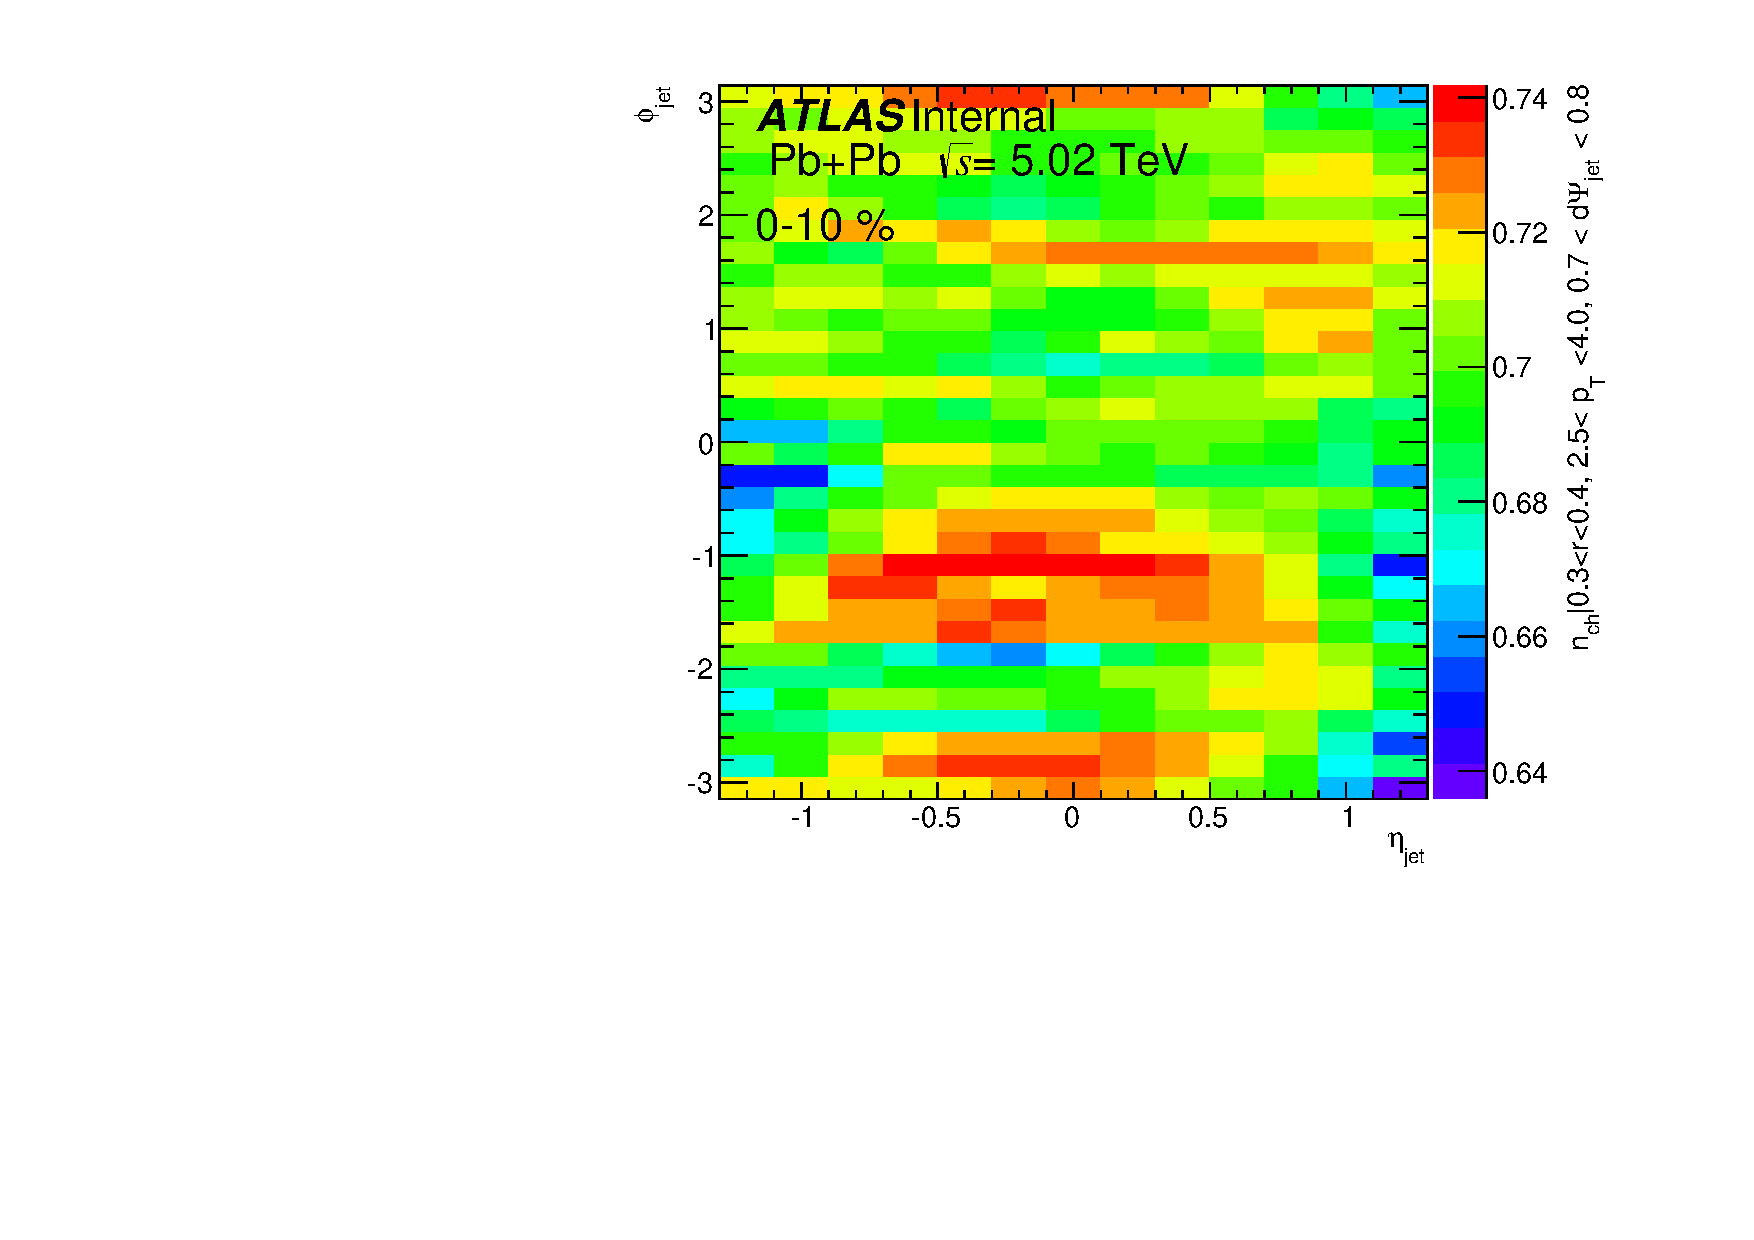
\includegraphics[width=0.33\textwidth]{figures_UE/h_UE_dR6_dPsi7_pt5_cent0.pdf}&
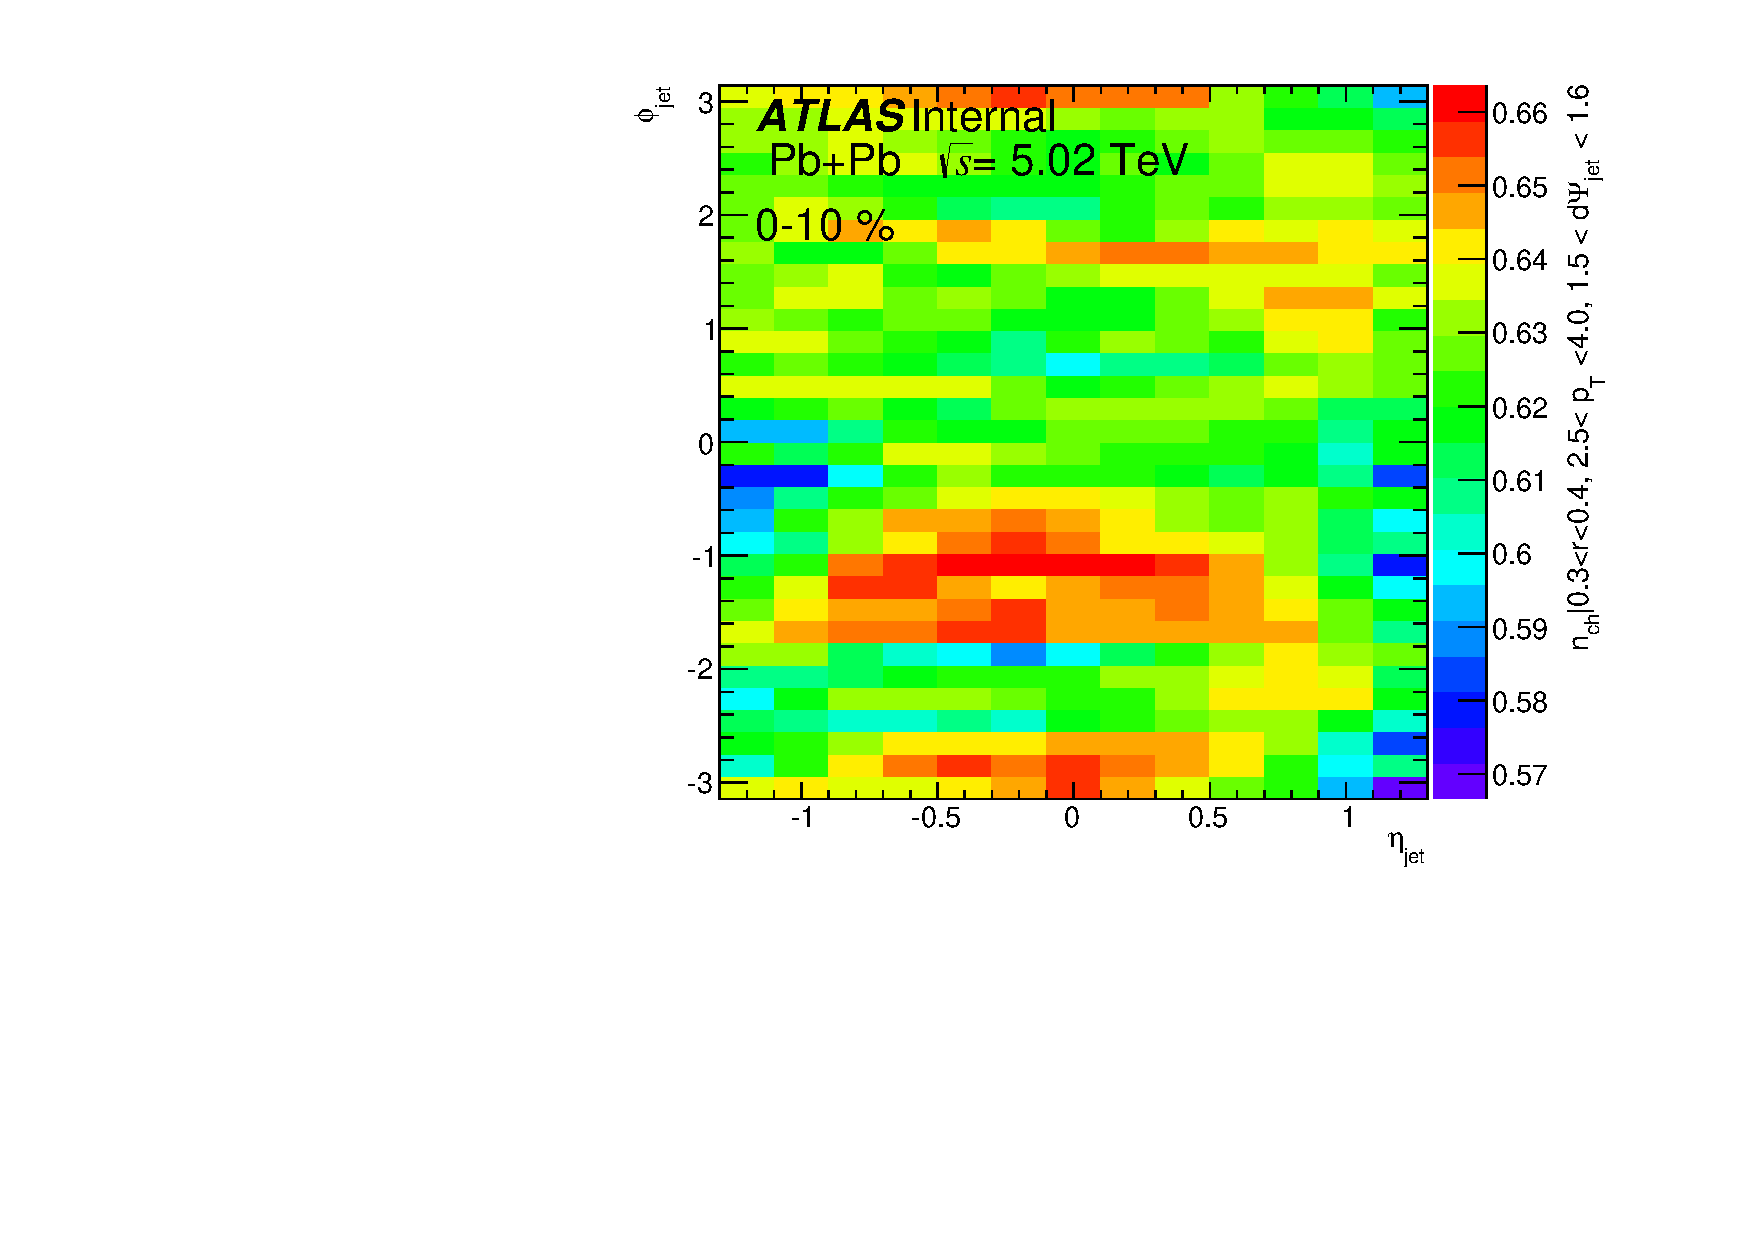
\includegraphics[width=0.33\textwidth]{figures_UE/h_UE_dR6_dPsi15_pt5_cent0.pdf} \\
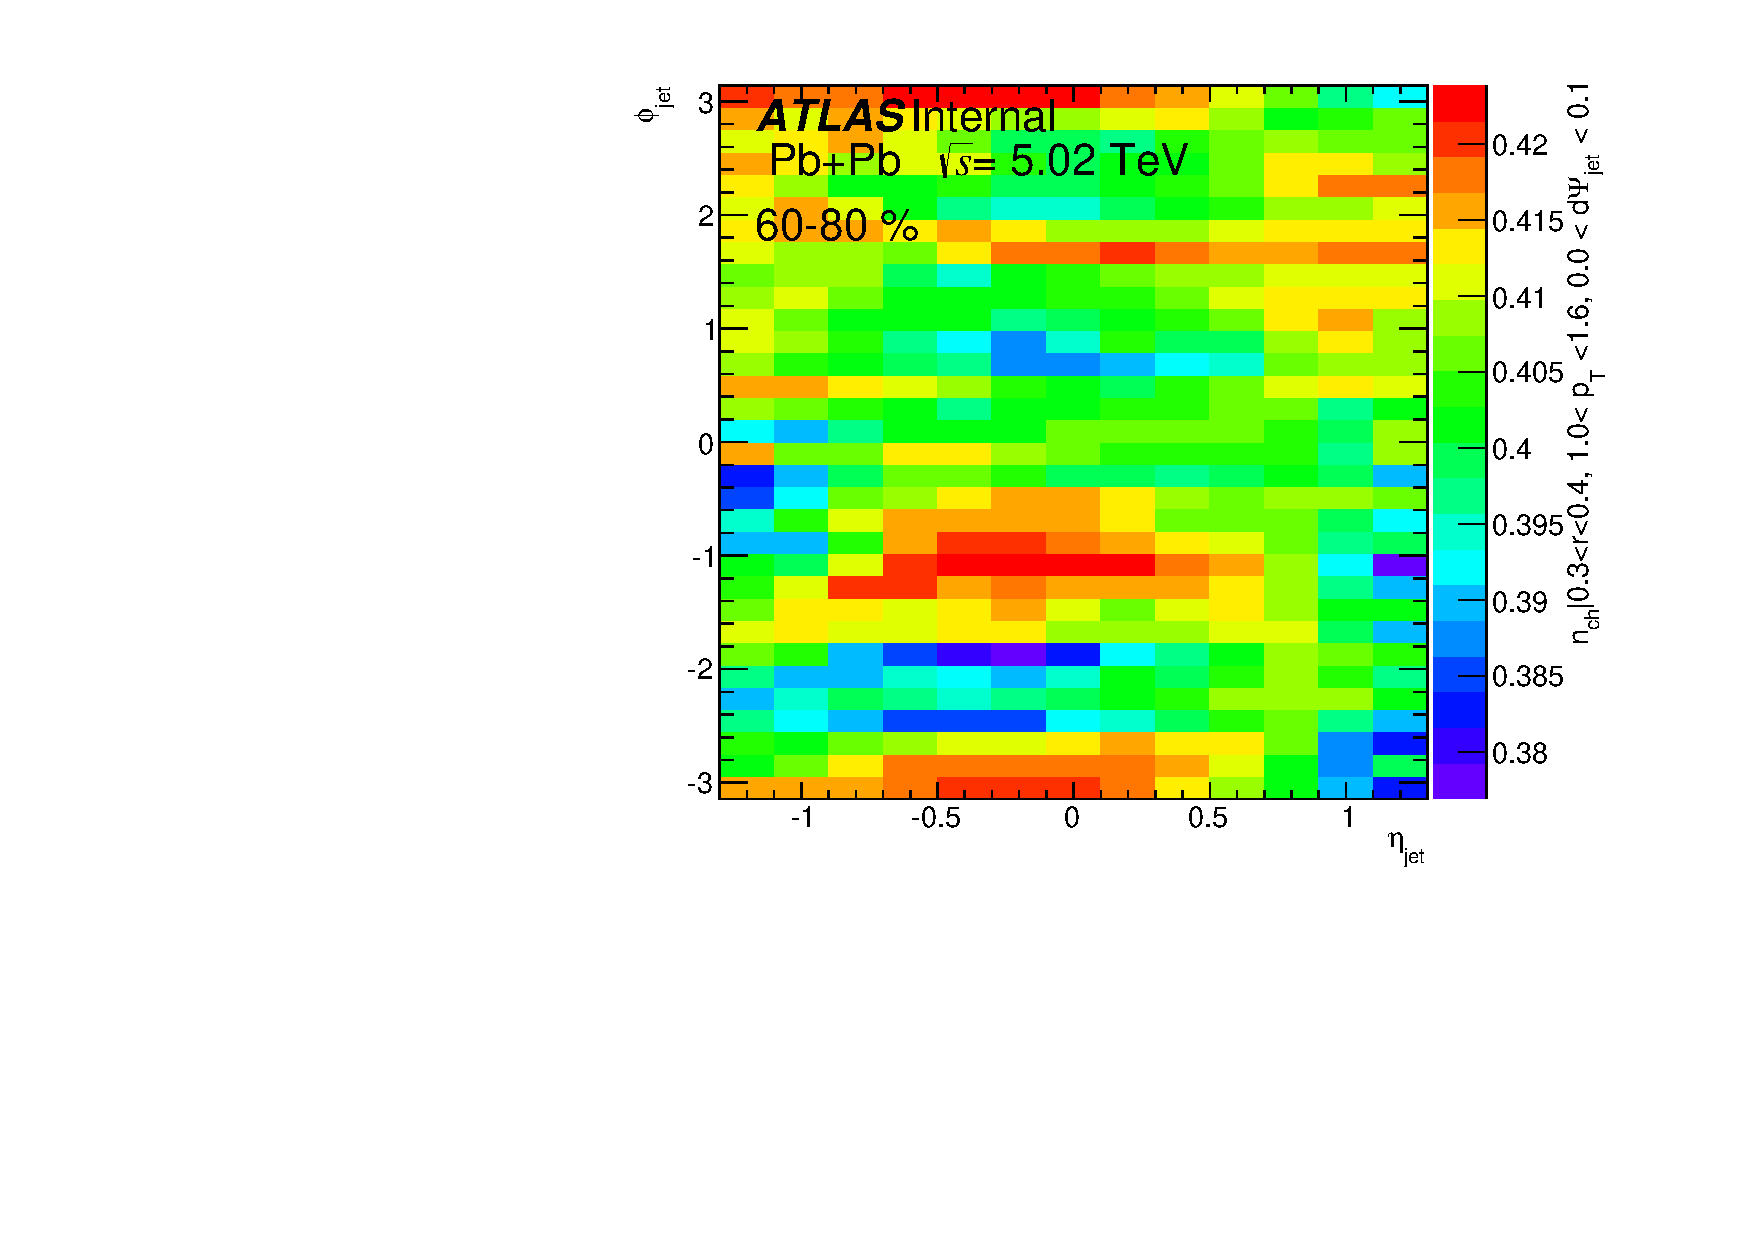
\includegraphics[width=0.33\textwidth]{figures_UE/h_UE_dR6_dPsi0_pt3_cent5.pdf} &
\includegraphics[width=0.33\textwidth]{figures_UE/h_UE_dR6_dPsi7_pt3_cent5.pdf}&
\includegraphics[width=0.33\textwidth]{figures_UE/h_UE_dR6_dPsi15_pt3_cent5.pdf} \\
\includegraphics[width=0.33\textwidth]{figures_UE/h_UE_dR6_dPsi0_pt5_cent5.pdf} &
\includegraphics[width=0.33\textwidth]{figures_UE/h_UE_dR6_dPsi7_pt5_cent5.pdf}&
\includegraphics[width=0.33\textwidth]{figures_UE/h_UE_dR6_dPsi15_pt5_cent5.pdf} \\
\end{tabular}}
\caption{
Per jet $\nchUE^{\mathrm{MB}}$ distributions of charged particles evaluated in the core of the jet ($0.3<r<0.4$) in MB events in three different intervals of angular distance with respect to the reaction plane angle going from left to right for two different selection of charged particle \pt\ and for two different centrality intervals.}
\label{fig:nchcore2}
\end{figure}

\begin{figure}[ht]
\centerline{
\begin{tabular}{ccc}
\includegraphics[width=0.33\textwidth]{figures_UE/h_UE_dR12_dPsi0_pt3_cent0.pdf} &
\includegraphics[width=0.33\textwidth]{figures_UE/h_UE_dR12_dPsi7_pt3_cent0.pdf}&
\includegraphics[width=0.33\textwidth]{figures_UE/h_UE_dR12_dPsi15_pt3_cent0.pdf} \\
\includegraphics[width=0.33\textwidth]{figures_UE/h_UE_dR12_dPsi0_pt5_cent0.pdf} &
\includegraphics[width=0.33\textwidth]{figures_UE/h_UE_dR12_dPsi7_pt5_cent0.pdf}&
\includegraphics[width=0.33\textwidth]{figures_UE/h_UE_dR12_dPsi15_pt5_cent0.pdf} \\
\includegraphics[width=0.33\textwidth]{figures_UE/h_UE_dR12_dPsi0_pt3_cent5.pdf} &
\includegraphics[width=0.33\textwidth]{figures_UE/h_UE_dR12_dPsi7_pt3_cent5.pdf}&
\includegraphics[width=0.33\textwidth]{figures_UE/h_UE_dR12_dPsi15_pt3_cent5.pdf} \\
\includegraphics[width=0.33\textwidth]{figures_UE/h_UE_dR12_dPsi0_pt5_cent5.pdf} &
\includegraphics[width=0.33\textwidth]{figures_UE/h_UE_dR12_dPsi7_pt5_cent5.pdf}&
\includegraphics[width=0.33\textwidth]{figures_UE/h_UE_dR12_dPsi15_pt5_cent5.pdf} \\
\end{tabular}}
\caption{
Per jet $\nchUE^{\mathrm{MB}}$ distributions of charged particles evaluated in the core of the jet ($1.0<r<1.2$) in MB events in three different intervals of angular distance with respect to the reaction plane angle going from left to right for two different selection of charged particle \pt\ and for two different centrality intervals.}
\label{fig:nchcore3}
\end{figure}


The UE contribution needs to be further corrected for effects the correlation between UE and JER and correlation of the production of secondary particles~\footnote{Secondary particles comes from weak decays of $\Lambda$, $K_{S}$, $\Xi$, $\Sigma$, $\Omega$ and from particles created in interactions with the material.} with the jet production.
   
Since the MC samples utilize the overlay procedure, where the real MB \PbPb\ collisions are used overlaid onto PYTHIA di-jets events, the UE distribution is the same as in data. The UE distributions thus can be alternatively calculated in MC samples from tracks that do not have an associated truth particle, $\fd \nchUE^{\mathrm{TM}}/ \fd \pTch$. This allowed us to study the size of the UE as a function of $r$ with respect to the jet axis. The UE estimated using this method is also needed to correct for the correlation between UE and JER and the enhancement of the rate of secondary particles in the jet which will be described below. The UE distribution normalized to unit area plotted as a function of $r$ with respect to the jet axis is shown in Fig.~\ref{fig:UEdR} for the lowest track \pt\ interval where the contribution of the UE is the largest. The two distributions represent the UE with and without the secondary particles. The UE strongly decreases with decreasing number of binary nucleon-nucleon as the collision centrality decreases. Only a very small dependence on the $r$ is seen for the UE when the secondary particles are not included. A small effect is expected as result of the pseudorapidity distribution of jets is enhanced towards the mid-rapidity region and the yields of UE particles decreases as a function of $\eta$, i.e. towards large $\Delta R$. As the secondary particles are generated by primary PYTHIA particles it is expected to see the enhancement towards the core of the jet when the multiplicity of primary particles is increased.      
  
  \begin{figure}[ht]
     \centerline{
        \includegraphics[width=0.9\textwidth]{figures_UE/UE_v_dR_pt1GeV.pdf}
     }
     \caption{UE estimated from tracks which do not have an associated truth particle in jet with \pt\ from 126 to 158 GeV and for the lowest track \pt\ interval (1--1.58 GeV). The two different distribution shows the UE with and without the contribution from the secondary particles.}
     \label{fig:UEdR}
  \end{figure}   


The interplay between the UE and the JER will be described in this paragraph and is discussed in details in Ref.~\cite{ATLAS-COM-PHYS-2012-1653}. Due to the steeply falling nature of the jet \pt\ spectra, the smearing due to jet energy resolution leads to a net migration of jets from lower \pt\ to higher \pt\ values (hereafter referred to as ``upfeeding'') such that a jet reconstructed with a given \pTrec\ will correspond, on average, to a lower truth jet \pT, \avgpttrue. The upfeeding was observed to induce in the MC a difference between the UE yields determined using the MB events and the actual UE contribution to reconstructed jets. The magnitude of this difference was found to be centrality dependent and exhibited a weak \pTjet\ dependence. That difference was found to result from
intrinsic correlations between the UE contribution to the yield of particles measured inside the jet and the MC \pTjet\ shift, $\Delta p_{\mathrm{T}}^{\mathrm{jet}}= \pTrec - \pTtrue$.  In particular, jets with positive (negative) $\Delta p_{\mathrm{T}}^{\mathrm{jet}}$ were found to have an UE contribution larger (smaller) than jets with $\Delta p_{\mathrm{T}}^{\mathrm{jet}} \sim 0$.  

\begin{figure}[ht]
\centerline{
\includegraphics[page=2,width=1.\textwidth]{figures_UE/UE_factors.pdf} \\
}
\caption{
The multiplicative correction factors that correct for the correlation between the UE and the JER, fake and secondary particles in different centrality classes and $ 0.05 < r < 0.10$.}
\label{fig:UEweights_r2}
\end{figure}

\begin{figure}[ht]
\centerline{
\includegraphics[page=6,width=1.\textwidth]{figures_UE/UE_factors.pdf} \\
}
\caption{
The multiplicative correction factors that correct for the correlation between the UE and the JER, fake and secondary particles in different centrality classes and $ 0.25 < r < 0.30$.}
\label{fig:UEweights_r6}
\end{figure}


\begin{figure}[ht]
\centerline{
\includegraphics[page=1,width=1.\textwidth]{figures_UE/UE_factors_r.pdf} \\
}
\caption{
The multiplicative correction factors that correct for the correlation between the UE and the JER, fake and secondary particles in different centrality classes, as a function of $r$ for $126 < \ptjet < 158 \GeV$.}
\label{fig:UEweights_r_jet0}
\end{figure}

  
  To correct for this effect, the centrality-, $\pTjet$-, $r-$ and $\pTch$-dependent multiplicative correction factors were applied on $\fd \nchUE^{\mathrm{MB}}/ \fd \pTch$ distributions. 
  These multiplicative factors, $1/w_{\mathrm{UE}}$, were estimated as a ratio of UE distributions calculated in MC samples from tracks within the area of a reconstructed jet which do not have an associated truth particle, $\Dptr_{f}$, and the UE distributions estimated using the MB events:  
  \begin{eqnarray}
  w_{\mathrm{UE}} (\pT) = \frac{\fd \nchUE^{\mathrm{MB}}/ \fd \pTch}{\fd \nchUE^{\mathrm{TM}}/ \fd \pTch}\bigg|_{\mathrm{MC}}
  \end{eqnarray}   
The example of those factors is plotted in Fig~\ref{fig:UEweights_r2}-\ref{fig:UEweights_r6}. The correction by construction corrects also for fakes and secondary contribution in the track \pT\ region 1-10~GeV in \PbPb\ collisions. These factors are also shown in Figure~\ref{fig:UEweights_r_jet0}, as a function of \rvar\ for different track \pt\ bins, for $126 < \ptjet\ < 158 \GeV$.  Outside that region and in \pp\ system fake contribution is corrected as described at the beginning of Section~\ref{sec:trackreco}.  The corrected UE distributions, $\fd \cnchUE / \fd \pTch$ are then subtracted from measured distributions both in MC and data as follows
 %
 \begin{eqnarray}
 \label{eq:Dptsub}
\frac{\fd n_{\mathrm{ch}}^{\mathrm{sub}}}{\fd \pTch}  = \frac{\fd n_{\mathrm{ch}}^{\mathrm{meas}}}{\fd \pTch} - \frac{1}{w_{\mathrm{UE}} (\pT)} \left( \frac{\fd \nchUE^{\mathrm{MB}}}{\fd \pTch} \right)  = \frac{\fd n_{\mathrm{ch}}^{\mathrm{meas}}}{\fd \pTch} - \frac{\fd \cnchUE}{\fd \pTch}
 \end{eqnarray}

The size of the $w_{\mathrm{UE}}$ correction is less than 1\% in kinematic regions where the UE is the largest, i.e. for low \pT\ charged particles inside the jet and at large $r$ distances for all track \pt. The absolute magnitude of the correction increases towards the higher track \pt\ in the jet core where the UE is smaller. This behavior originates from 1) the intrinsic correlations between the UE contribution to the yield of particles measured inside the jet and the MC \pTjet\ shift as it was discussed earlier; 2) the correlation of production of secondary particles with the jet.  The production of secondary particles is associated with presence of primary particles. Thus, the production of secondary particles is enhanced in the jet due to the higher density of primary particles compared to the regions outside a jet. This is shown in Fig.~\ref{fig:UEdR} where the UE evaluated in term of particles without matching to truth particles in MC with and without the contribution from secondary particles is presented and where the yield of secondary particles is significant only at smaller $dR$, i.e. within a jet.  Fig.~\ref{fig:UEdR} also shows that the relative yield of secondary particles to the yield of the UE particles is increasing with decreasing collisions centrality. Furthermore, the relative contribution of secondary particles to the UE increases with the track \pT\ as the fraction of the secondary particles decreases only slowly with the increasing track \pT (Figs.\ref{fig:fakeratepbpb}), however, the UE decreases strongly with the increasing track \pT\ (Fig.\ref{fig:UEimpact_r2}-\ref{fig:UEimpact_r6}). This results in lower UE contribution estimated using the MB collisions where tracks are not associated to a jet. The two methods give almost identical UE at angles outside the $R=0.4$ jet as the role of the two effect discussed here decreases.
     

The impact of the underlying event and fake track subtraction on the \Dptr\ distributions is shown in 
Figure~\ref{fig:UEimpact_r2}-\ref{fig:UEimpact_r6}.
The magnitude of this correction is the largest for low track \pt\ in central \pbpb\ collisions and the largest annulus. In the most extreme case the S/B ratios can be as low as 1/100.  The size of the correction decreases rapidly with increasing track \pt, decreasing centrality and towards the core of the jet.  In \pp\ collisions the magnitude of the fake track subtraction
is always much less than 5\%.

\begin{figure}[ht]
\centerline{
 \includegraphics[page=2,width=0.8\textwidth]{figures_UE/ChPS_B2S_PbPb_data.pdf} \\
}
 \caption{Ratio between the raw \Dptr\ distributions without and with the UE 
        subtraction in different centrality classes and different jet \pT\ intervals for $ 0.05 < r < 0.10$.}
    \label{fig:UEimpact_r2}
 \end{figure}

\begin{figure}[ht]
\centerline{
\includegraphics[page=6,width=0.8\textwidth]{figures_UE/ChPS_B2S_PbPb_data.pdf} \\
}
\caption{Ratio between the raw \Dptr\ distributions without and with the UE
subtraction in different centrality classes and different jet \pT\ intervals for $ 0.25 < r < 0.30$.}
\label{fig:UEimpact_r6}
\end{figure}


The basic performance of the UE subtraction has been tested in the MC overlay dataset. The closure test was performed using the MC overlay sample that has the same UE as in the data and will be discussed in the next subsection. The truth \Rdptr\ distributions were compared to fully corrected \Rdptr\ distributions where the same UE contribution is subtracted by the same method as used in the data (see Figure~\ref{fig:PbPb_ChPS_closure}). From the above mentioned tests we have concluded that the UE subtraction procedure is correct and works well. The UE estimate is subjected to variation as part of the systematic uncertainties. For the \pp\ data, we have not performed any UE subtraction.

\clearpage

\subsection{Unfolding}
\label{sec:unfolding}

Instrumental effects are corrected by an unfolding procedure. This analysis uses three separate unfolding procedures that are discussed in this section. 
\begin{itemize}

\item One dimensional unfolding for the \ptjet\ spectra for the normalization.
\item Two dimensional Bayesian unfolding in \pttrk\ and \ptjet for jet \pt\ dependent yields of charged particles.
\item Bin by bin correction for the jet and track position resolution.

\end{itemize}

%The closure of the unfolding is checked by applying the response matrices from MC to the reconstructed spectra in MC.

\subsubsection{One Dimensional Unfolding for Jet Spectra}
\label{sec:1dunfolding}
The charged particle spectra need to be normalized by the number of jets in given jet \pt\ interval. Thus, the jet spectra needs to be corrected for bin migration due to the finite JER by unfolding procedure. 
%Since the primary effect to be unfolded for is the jet energy resolution (which is a much larger effect than the \pt\ resolution for charged tracks), one dimensional or bin-by-bin unfolding might seem to be appropriate. 
The unfolding is done via a one dimensional Bayesian unfolding procedure with 4 iterations implemented as part of the RooUnfold~\cite{Adye:2011gm} package. The \pp\ and \PbPb\ MC samples are used to construct two dimensional response matrices in terms of \ptjettruth\ and \ptjetreco. These matrices can be seen in Fig:\ref{fig:PbPb_jetspect_respmatrix}-\ref{fig:pp_jetspect_respmatrix} and are evaluated separately for \pp\ and in different centrality intervals for \PbPb\ collisions. The performance of the unfolding was verified by closure test, where the MC sample was used to derive the responses matrices that were then used to unfold the reconstructed jet spectra. Such unfolded distributions are than compared to those evaluated using truth jets. The jet spectra and MC closure is shown in Fig:\ref{fig:PbPb_jetspect_closure}-\ref{fig:pp_jetspect_closure}, as a function of \ptjet\ for jets in the. $|y| < $ 1.3 region. A good recovery of the truth distribution is seen, the MC closure is well within 1\% for \pbpb\ and \pp\ MC samples.

\begin{figure}[ht]
\centering
\includegraphics[page=5, width=0.9\textwidth]{figures_corrections/resp_matrix_jet_PbPb_MC.pdf}
\caption{The response matrices in terms of \ptjetreco\ and \ptjettruth\ in the jet $|y| < $1.3 region, in data overlay \pbpb\ MC samples. Each panel is a different centrality bin.}
\label{fig:PbPb_jetspect_respmatrix}
\end{figure}

\begin{figure}[ht]
\centering
\includegraphics[page=5, width=0.55\textwidth]{figures_corrections/resp_matrix_jet_pp_MC.pdf}
\caption{The response matrices in terms of \ptjetreco\ and \ptjettruth\ in the jet $y < $1.3 region, in \pp\ MC samples.}
\label{fig:pp_jetspect_respmatrix}
\end{figure}

\begin{figure}[ht]
\centering
\includegraphics[page=5, width=0.9\textwidth]{figures_corrections/spect_closure_PbPb_MC.pdf}
\caption{The jet spectra and MC closure as a function of \ptjet\ in the jet $|y| < $1.3 region, in data overlay \pbpb\ MC samples. The closure is seen to be well within 1\%. Each panel is a different centrality bin.}
\label{fig:PbPb_jetspect_closure}
\end{figure}

\begin{figure}[ht]
\centering
\includegraphics[page=5, width=0.55\textwidth]{figures_corrections/spect_closure_pp_MC.pdf}
\caption{The jet spectra and MC closure as a function of \ptjet\ in the jet $|\eta| < $1.3 region, in \pp\ MC samples. The closure is seen to be well within 1\%.}
\label{fig:pp_jetspect_closure}
\end{figure}



\subsubsection{Two Dimensional Unfolding for Charged Particle Spectra}
\label{sec:2dunfolding}


Observed correlation between the jet response in the detector and the jet fragmentation necessitates a two dimensional unfolding~\cite{ATLAS502FFConf}. 
%The dependence of the jet response on the fragmentation pattern of a particular jet has been studied extensively in ATLAS.
For example, gluon jets, which have in general a softer fragmentation function, are observed to have a lower energy response than quark jets~\cite{Aad:2014bia}.  The Global Sequential Calibration to the \pp\ jet collections~\cite{ATLAS:2015oia}, reduces the fragmentation dependence to the JES, but these calibrations are not available for the HI jet collections used in this analysis.

We use the RooUnfold~\cite{Adye:2011gm} implementation of the two dimensional iterative Bayesian unfolding~\cite{D'Agostini:1994zf} with 4 iterations. The MC \pbpb\ and \pp\ samples are used to construct a 4-dimensional response matrix in \pttrktruth, \ptjettruth, \pttrkreco, and \ptjetreco, shown in Fig:\ref{fig:PbPb_ChPS_respmatrix}-\ref{fig:pp_ChPS_respmatrix}. The response matrix $A_{ijkl}$ describes the probability that event from the truth track \pt\  bin $j$ and truth jet \pT\ bin $l$ is found in reconstructed bin $i$,$k$:
\begin{equation}
\mu_{jl} = \sum_{i,k} A_{ijkl}x^{\text{truth}}_{jl}.
\end{equation} 


\begin{figure}[ht]
\centering
\includegraphics[page=5, width=1.0\textwidth]{figures_corrections/resp_matrix_ChPS_PbPb_MC.pdf}
\caption{The response matrices in terms of \ptjetreco, \ptjettruth, \pttrkreco, and \pttrktruth, for reconstructed track - reconstructed jet pairs, that have 0.20 $< r < $0.25, in data overlay \pbpb\ MC samples. Each panel is a different centrality bin.}
\label{fig:PbPb_ChPS_respmatrix}
\end{figure}

\begin{figure}[ht]
\centering
\includegraphics[page=5, width=1.0\textwidth]{figures_corrections/resp_matrix_ChPS_pp_MC.pdf}
\caption{The response matrix in terms of \ptjetreco, \ptjettruth, \pttrkreco, and \pttrktruth, for reconstructed track - reconstructed jet pairs, that have 0.20 $< r < $0.25, in \pp\ MC samples}
\label{fig:pp_ChPS_respmatrix}
\end{figure}


\subsubsection{Bin-by-bin correction for Angular resolution}
\label{sec:bbbcorrection}

There is an additional unfolding procedure applied in this analysis to correct for the jet and the track position resolution that results in the migration in angular distance $r$. The migration is dominated by the poor jet angular resolution (Fig.\ref{Fig:PerformancepbpbJPReta0p4}-\ref{Fig:PerformancepbpbJPRphi0p4}), since the track angular resolution (Fig.\ref{fig:PbPb_trk_eta_res}-\ref{fig:PbPb_trk_phi_res}) is very good.

\begin{figure}[ht]
\centering
\includegraphics[width=0.9\textwidth]{figures_corrections/trk_res_eta_ppTight.pdf}
\caption{The $\eta$ resolution of the tracker in different $\eta$ bins for data overlay \pbpb\ MC samples. The different curves are different centralities, and it can be seen that there is no centrality dependence.}
\label{fig:PbPb_trk_eta_res}
\end{figure}

\begin{figure}[ht]
\centering
\includegraphics[width=0.9\textwidth]{figures_corrections/trk_res_phi_ppTight.pdf}
\caption{The $\phi$ resolution of the tracker in different $\phi$ bins for data overlay \pbpb\ MC samples. The different curves are different centralities, and it can be seen that there is no centrality dependence.}
\label{fig:PbPb_trk_phi_res}
\end{figure}

The correction factors are derived using response matrices that correlate the reconstructed and truth angular distance $r$. These matrices are evaluated for different jet and track \pT\ in different centrality classes. Examples of the response matrices are shown in Fig~\ref{fig:PbPb_bbb_2d_response} and Fig.~\ref{fig:pp_bbb_2d_response} for \pbpb\ and \pp\ MC samples. The bin-by-bin correction procedure is applied to \Dptr\ distribution unfolded to the particle level in terms of track and jet \pT\ by the two unfoldings discussed above. Thus, the correction factors for angular resolution were derived using the the reconstructed jets and tracks where the reconstructed jet and track \pT\ is replaced by the corresponding truth \pT. The bin-by-bin factors are then estimated as ratio of projections from the response matrices on the truth and reconstructed axis. These correction factors are shown in Fig.~\ref{fig:pos_corr_factors_PbPb_c0} and Fig.~\ref{fig:pos_corr_factors_pp} for \pbpb\ and \pp\ collisions as a function of \rvar.

\begin{figure}[ht]
\centering
\includegraphics[page=1, width=0.9\textwidth]{figures_corrections/ShapeResponse2D_PbPb.pdf}
\caption{The response matrix for the bin by bin correction applied to the unfolded charged particle spectra. This accounts for the jet position resolution. Each panel is a different \pttrk\ bin, for $126 < \ptjet\ < 158$ GeV jets, in central collisions from data overlay \pbpb\ MC samples}
\label{fig:PbPb_bbb_2d_response}
\end{figure}

\begin{figure}[ht]
\centering
\includegraphics[page=1, width=0.9\textwidth]{figures_corrections/ShapeResponse2D_pp.pdf}
\caption{The response matrix for the bin by bin correction applied to the unfolded charged particle spectra. This accounts for the jet position resolution. Each panel is a different \pttrk\ bin, for $126 < \ptjet\ < 158$ GeV jets, from \pp\ MC samples}
\label{fig:pp_bbb_2d_response}
\end{figure}


\begin{figure}[ht]
\centering
\includegraphics[page=1, width=0.9\textwidth]{figures_corrections/RatioProj_PbPb}
\caption{The correction factors applied to the unfolded charged particle spectra, shown for the most central collisions, as a function of $r$, with each panel showing a different track \pt\ bin, and each curve showing a different \ptjet\ range. These factors correct for the jet position resolution in \pbpb\ collisions.}
\label{fig:pos_corr_factors_PbPb_c0}
\end{figure}

\begin{figure}[ht]
\centering
\includegraphics[page=1, width=0.9\textwidth]{figures_corrections/RatioProj_pp}
\caption{The correction factors applied to the unfolded charged particle spectra, as a function of $r$, with each panel showing a different track \pt\ bin, and each curve showing a different \ptjet\ range. These factors correct for the jet position resolution in \pp\ collisions..}
\label{fig:pos_corr_factors_pp}
\end{figure}


The \Dptr\ distributions at various stages of the analysis in \pp\ MC and data (Fig:\ref{fig:evol_pp}), and \pbpb\ MC and data (Fig:\ref{fig:evol_PbPb_MC}-\ref{fig:evol_PbPb_data}) are also shown.

\begin{figure}[ht]
   \centerline{
      \begin{tabular}{c}
	\includegraphics[page=5, width=0.5\textwidth]{figures_corrections/evol_pp_MC.pdf}
	\includegraphics[page=5, width=0.5\textwidth]{figures_corrections/evol_pp_data.pdf}
   \end{tabular}
   }
   \caption{The evolution of the \Dptr\ distributions for \pp\ MC (left) and data (right) as various corrections are applied. The spectra is shown for tracks with $0.05 < \Delta r < 0.10$ away from the jet axis, for $126 < \ptjet < 158$ GeV. The ratios showing the effect of the unfolding and bin by bin corrections (left and right), as well as the MC closure (left) are shown in the lower half of the panels. }
      \label{fig:evol_pp}
   \end{figure}


\begin{figure}[ht]
\centerline{
\includegraphics[page=5, width=0.85\textwidth]{figures_corrections/evol_PbPb_MC.pdf}
}
\caption{The evolution of the \Dptr\ distributions for \PbPb\ MC as various corrections are applied. The spectra is shown for tracks with $0.05 < \Delta r < 0.10$ away from the jet axis, for $126 < \ptjet < 158 $GeV. The ratios showing the effect of the subtraction, unfolding and bin by bin correction (left and right), as well as the MC closure (left) are shown in the lower half of the panels. The different panels are different centrality selections.}
\label{fig:evol_PbPb_MC}
\end{figure}

\begin{figure}[ht]
\centerline{
\includegraphics[page=5, width=0.85\textwidth]{figures_corrections/evol_PbPb_data.pdf}
}
\caption{The evolution of the \Dptr\ distributions for \PbPb\ data (bottom six panels) as various corrections are applied. The spectra is shown for tracks with $0.05 < \Delta r < 0.10$ away from the jet axis, for $126 < \ptjet < 158 $GeV. The ratios showing the effect of the subtraction, unfolding and bin by bin correction (left and right), as well as the MC closure (left) are shown in the lower half of the panels. The different panels are different centrality selections.}
\label{fig:evol_PbPb_data}
\end{figure}


The MC closure of the charged particle spectra as a function of \pt\ in \pp\ and data overlay \pbpb\ MC samples can be seen in Fig:\ref{fig:PbPb_ChPS_closure}-\ref{fig:pp_ChPS_closure}, and is well within 1\%.

\begin{figure}[ht]
\centering
\includegraphics[page=5, width=1.0\textwidth]{figures_corrections/ChPS_final_PbPb_MC.pdf}
\caption{The charged particle spectra and MC closure as a function of \pttrk\ for different \ptjet\ bins, reconstructed track - reconstructed jet pairs, that have 0.20 $< r < $0.25, in data overlay \pbpb\ MC samples. Each panel is a different centrality bin. The closure is seen to be well within 1\%.}
\label{fig:PbPb_ChPS_closure}
\end{figure}

\begin{figure}[ht]
\centering
\includegraphics[page=5, width=0.55\textwidth]{figures_corrections/ChPS_final_pp_MC.pdf}
\caption{The charged particle spectra and MC closure as a function of \pttrk\ for different \ptjet\ bins, reconstructed track - reconstructed jet pairs, that have 0.20 $< r < $0.25, in \pp\ MC samples. The closure is seen to be well within 1\%}
\label{fig:pp_ChPS_closure}
\end{figure}

